%\subsubsection{PFCA standards}
%Another source of error could be the homogeneity of the PFAS standards. If the standards were not shaken (vortexed) properly before pipetting, the PFAS solution could be unevenly dissolved and thus cause inconsistent concentrations pipetted into each centrifuge tube. This can be particularly significant for the long-chain PFCAs which are less soluble than the short-chain ones. 

%What we did to overcome this, analyzed the standards themselves and compared with calculated concentrations. 

\begin{table}
\centering
\caption{pH, conductivity, TOC and total nitrogen, cation exchange capacity (CEC) for the soil blank used in the batch tests}
\label{tab:soilsummary}
\adjustbox{max width=\textwidth}{
\begin{tabular}{llllll}
\textbf{pH ($\mathrm{H_2O}$)} & \textbf{pH (0.01 M $\mathrm{CaCl_2}$)} & \textbf{Conductivity ($\mu S/cm$)} & \textbf{TOC (\%)} & \textbf{N-tot (\%)} & CEC (meqv/100g) \\
5.38    ± 0.02    & 4.36  ± 0.01               & 23.33  ± 0.05                 & 1.32  ± 0.03      & 0.11  ± 0.003    & 2.62 ± 0.07  
\end{tabular}}
\end{table}

\begin{table}
\centering
\caption{Surface area and pore volume for the biochars produced for the batch tests.}
\adjustbox{max width=\textwidth}{
\label{tab:SAPV}
\begin{tabular}{llllll}
\toprule
Biochar  &  Pyrolysis  & \multicolumn{2}{c}{N\textsubscript{2} sorption} & \multicolumn{2}{c}{CO\textsubscript{2} sorption} \\  
         sorbent     &  temperature & \multicolumn{2}{c}{(pores \textgreater 1.5 nm)} & \multicolumn{2}{c}{(pores 0.4-1.5 nm)}\\ \cmidrule(l){3-4} \cmidrule(l){5-6}
              & (\textdegree C) & Surface area         & Pore volume         & Surface area          & Pore volume         \\
 &  & $\mathrm{m^2~g^{-1}}$  & cm\textsuperscript{3} g\textsuperscript{-1}           & $\mathrm{m^2~g^{-1}}$            & cm\textsuperscript{3} g\textsuperscript{-1}           \\ \midrule
ULS         & 700                    & 128         & 0.126          & 164.58          & 0.047          \\
CWC         & 700                    & 323         & 0.017          & 683.27          & 0.186          \\
DSL         & 700                    & 110         & 0.111          & 86.55           & 0.027         \\ \midrule
\end{tabular}}
\end{table}

\begin{table}
\caption{Effective cross-sectional diameter (D\textsubscript{eff}) and maximum diameter (D\textsubscript{max}) of TCs interpolated and extrapolated by linear regression from calculations performed by \citep{inoue2012size} on PFOA and other PFCAs with chain lengths 11-18.}
\centering
\begin{threeparttable}
\label{tab:molecsize}
\begin{tabular}{lcll}
\toprule
Compound & \begin{tabular}[l]{@{}l@{}}Carbon chain \\ length\end{tabular} & \begin{tabular}[c]{@{}l@{}}D\textsubscript{eff} \\ (nm)\end{tabular} & \begin{tabular}[c]{@{}l@{}}D\textsubscript{max} \\ (nm)\end{tabular} \\ \midrule
PFPeA    & 5                                                              & 0.45                                                 & 0.96                                                 \\
PFHxA    & 6                                                              & 0.50                                                 & 1.08                                                 \\
PFHpA    & 7                                                              & 0.56                                                 & 1.19                                                 \\
PFOA\textsuperscript{*}     & 8                                                              & 0.61                                                 & 1.36                                                 \\
PFNA     & 9                                                              & 0.67                                                 & 1.42                                                 \\
PFDA     & 10                                                             & 0.72                                                 & 1.54  \\ \bottomrule                                    
\end{tabular}
\begin{tablenotes}
\item \textsubscript{*} Calculated value from \citep{inoue2012size}
\end{tablenotes}
\end{threeparttable}
\end{table}

\begin{table}
\caption{Freundlich sorption parameters of single TC isotherms in CWC, ULS and DSL (n=9). The error is presented as standard error. All $K_F$ data are in units of $\mathrm{(\mu g/kg)/(\mu g/L)^{n_F}}$.}
\centering
\adjustbox{max width=\textwidth}{%
\begin{threeparttable}
\label{tab:summary_stats_single}
\begin{tabular}{llllllllllll}
\toprule
\multicolumn{1}{c}{Biochar} & \multicolumn{1}{c}{Compound} & \multicolumn{3}{c}{$log~K_{F,BC}$} & \multicolumn{3}{c}{$n_{F,BC}$} & \multicolumn{3}{c}{$r^2$} & $p$ \\ \midrule
CWC                                  & PFPeA                                 & 3.98        & ±        & 0.36        & 0.56      & ±      & 0.33      & 0.30       & ±       & 0.31            & -             \\
CWC                                  & PFHxA                     & 3.01        & ±        & 0.32        & 0.69      & ±      & 0.17      & 0.68       & ±       & 0.67               & **           \\
CWC                                  & PFHpA                     & 4.44        & ±        & 0.05        & 0.59      & ±      & 0.11      & 0.80       & ±       & 0.16               & **           \\
CWC                                  & PFOA                      & 5.06        & ±        & 0.08        & 0.39      & ±      & 0.05      & 0.90       & ±       & 0.10               & ***          \\
CWC                                  & PFNA                      & 4.88        & ±        & 0.04        & 0.65      & ±      & 0.04      & 0.98       & ±       & 0.05               & ***          \\
CWC                                  & PFDA                      & 5.22        & ±        & 0.07        & 0.45      & ±      & 0.04      & 0.94       & ±       & 0.08               & ***          \\
DSL                                  & PFPeA                     & 4.25        & ±        & 0.74        & 0.14      & ±      & 0.38      & 0.06       & ±       & 0.07               & -             \\
DSL                                  & PFHxA                     & 3.16        & ±        & 0.04        & 1.22      & ±      & 0.03      & 1.00       & ±       & 0.09               & ***          \\
DSL                                  & PFHpA                     & 4.67        & ±        & 0.06        & 0.57      & ±      & 0.09      & 0.86       & ±       & 0.13               & ***          \\
DSL                                  & PFOA                      & 5.12        & ±        & 0.02        & 0.60      & ±      & 0.02      & 0.99       & ±       & 0.03               & ***          \\
DSL                                  & PFNA                      & 5.33        & ±        & 0.03        & 0.80      & ±      & 0.07      & 0.94       & ±       & 0.08               & ***          \\
DSL                                  & PFDA                      & 5.61        & ±        & 0.02        & 0.61      & ±      & 0.02      & 0.99       & ±       & 0.03               & ***          \\
ULS                                  & PFPeA                     & 4.10        & ±        & 0.13        & 0.67      & ±      & 0.16      & 0.74       & ±       & 0.17               & **           \\
ULS                                  & PFHxA                     & 4.80        & ±        & 0.06        & 0.34      & ±      & 0.09      & 0.72       & ±       & 0.13               & **           \\
ULS                                  & PFHpA                     & 5.98        & ±        & 0.17        & 1.08      & ±      & 0.11      & 0.93       & ±       & 0.10               & ***          \\
ULS                                  & PFOA                      & 5.73        & ±        & 0.02        & 0.65      & ±      & 0.05      & 0.95       & ±       & 0.07               & ***          \\
ULS                                  & PFNA                      & 5.89        & ±        & 0.02        & 0.71      & ±      & 0.03      & 0.99       & ±       & 0.04               & ***          \\
ULS                                  & PFDA                      & 6.00        & ±        & 0.04        & 0.35      & ±      & 0.05      & 0.86       & ±       & 0.13               & ***     \\ \bottomrule    
\end{tabular}
\begin{tablenotes}
\item Significant codes: *** $\sim$ 0.001, ** $\sim$ 0.01, - $>$ 0.05 
\end{tablenotes}
\end{threeparttable}}
\end{table}

\begin{figure}
    \centering
    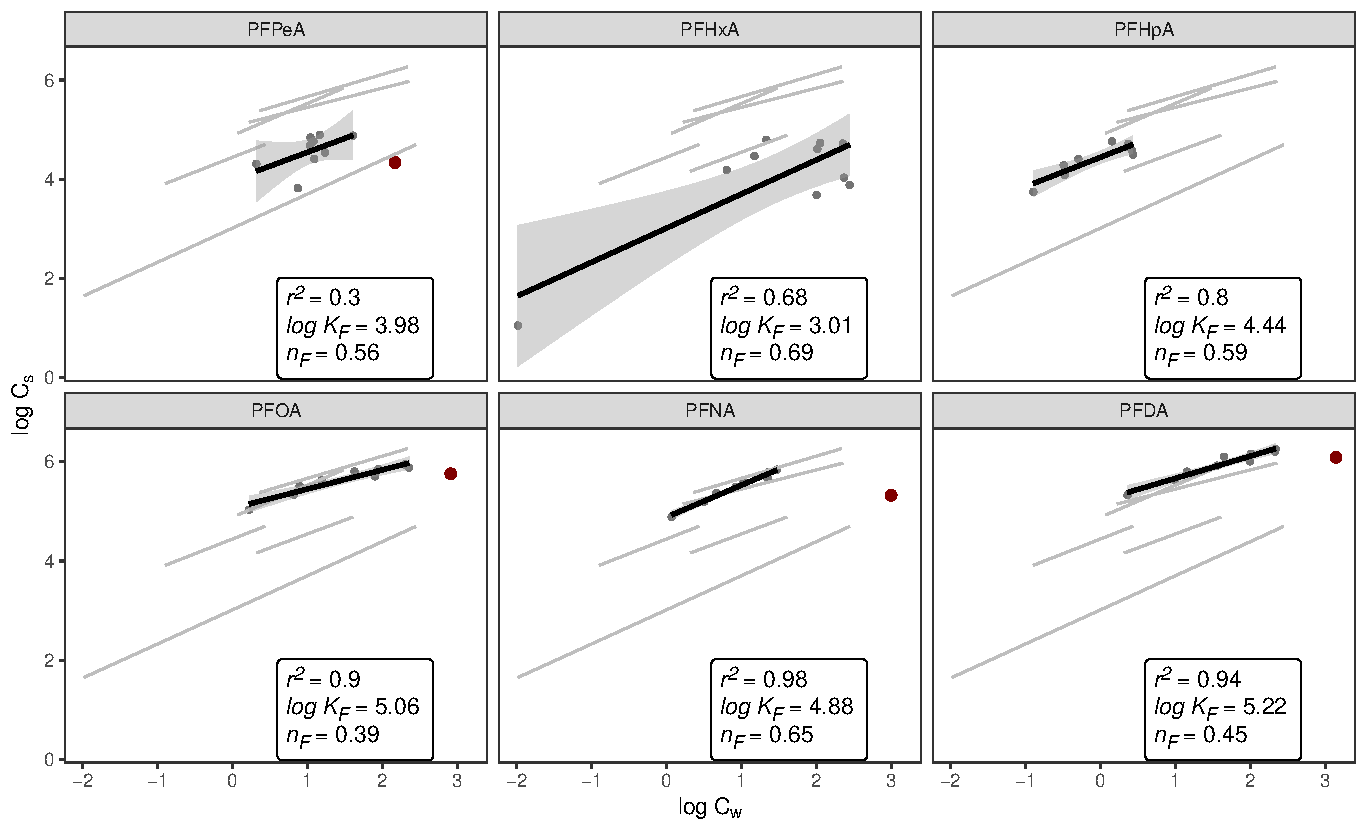
\includegraphics[width=\textwidth]{R/figs/CWC_facet_isotherm.pdf}
    \caption{Freundlich isotherms of TCs in CWC batch tests. Lines are obtained by linear regression.}
    \label{fig:CWC_isotherm2}
\end{figure}

\begin{figure}
    \centering
    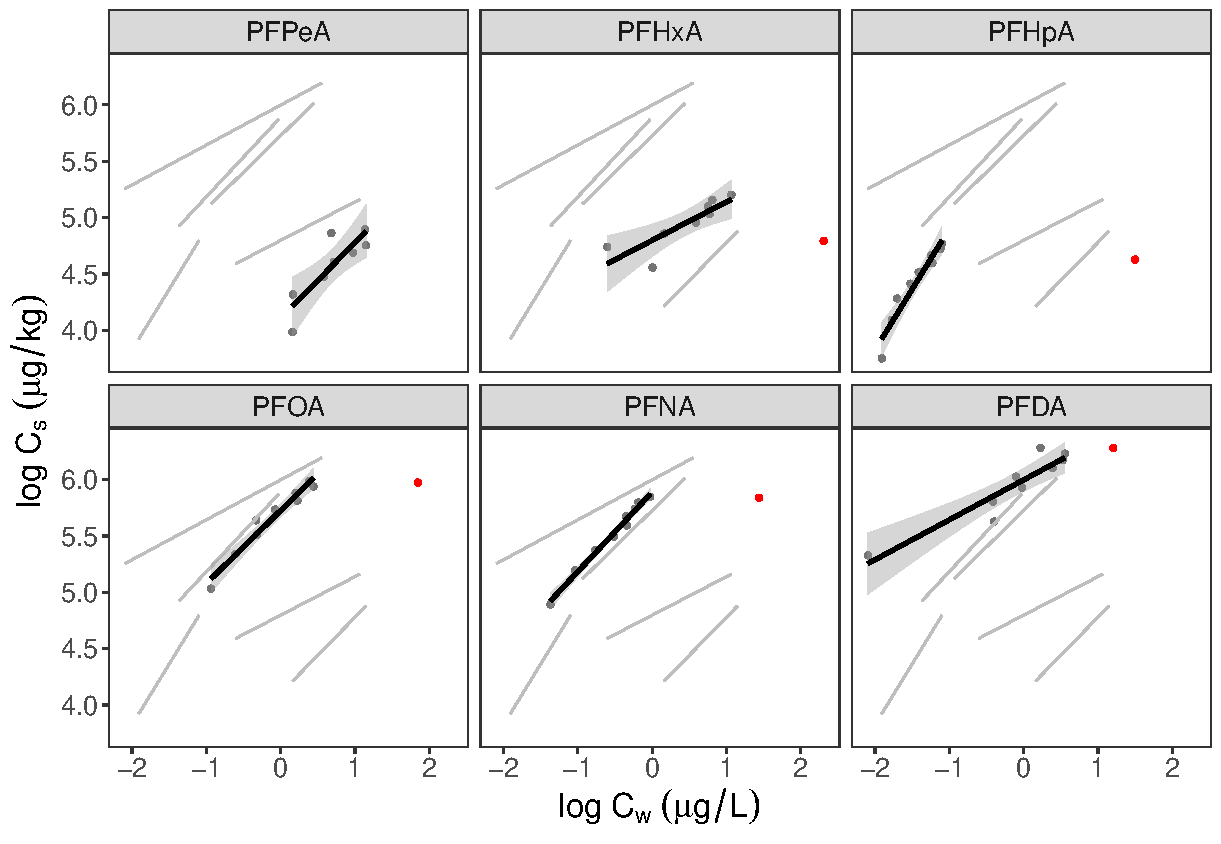
\includegraphics[width=\textwidth]{R/figs/ULS_facet_isotherm.pdf}
    \caption{Freundlich isotherms of TCs in ULS batch tests. Lines are obtained by linear regression.}
    \label{fig:ULS_isotherm2}
\end{figure}

\begin{figure}
    \centering
    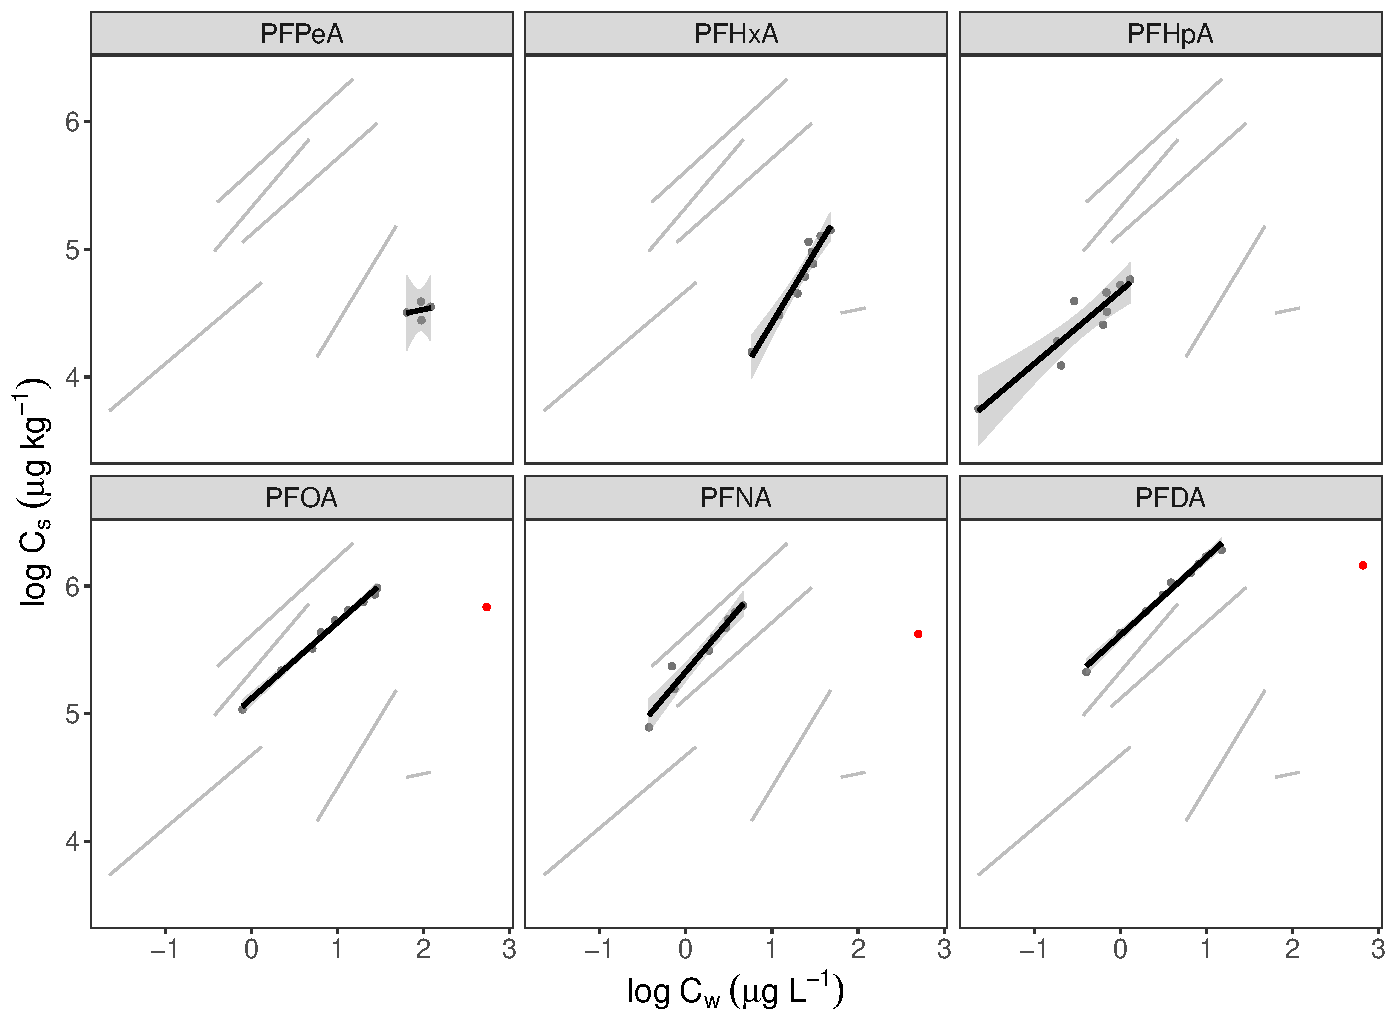
\includegraphics[width=\textwidth]{R/figs/DSL_facet_isotherm.pdf}
    \caption{Freundlich isotherms of TCs in DSL batch tests. Lines are obtained by linear regression.}
    \label{fig:DSL_isotherm2}
\end{figure}

\begin{figure}[tb]
    \centering
    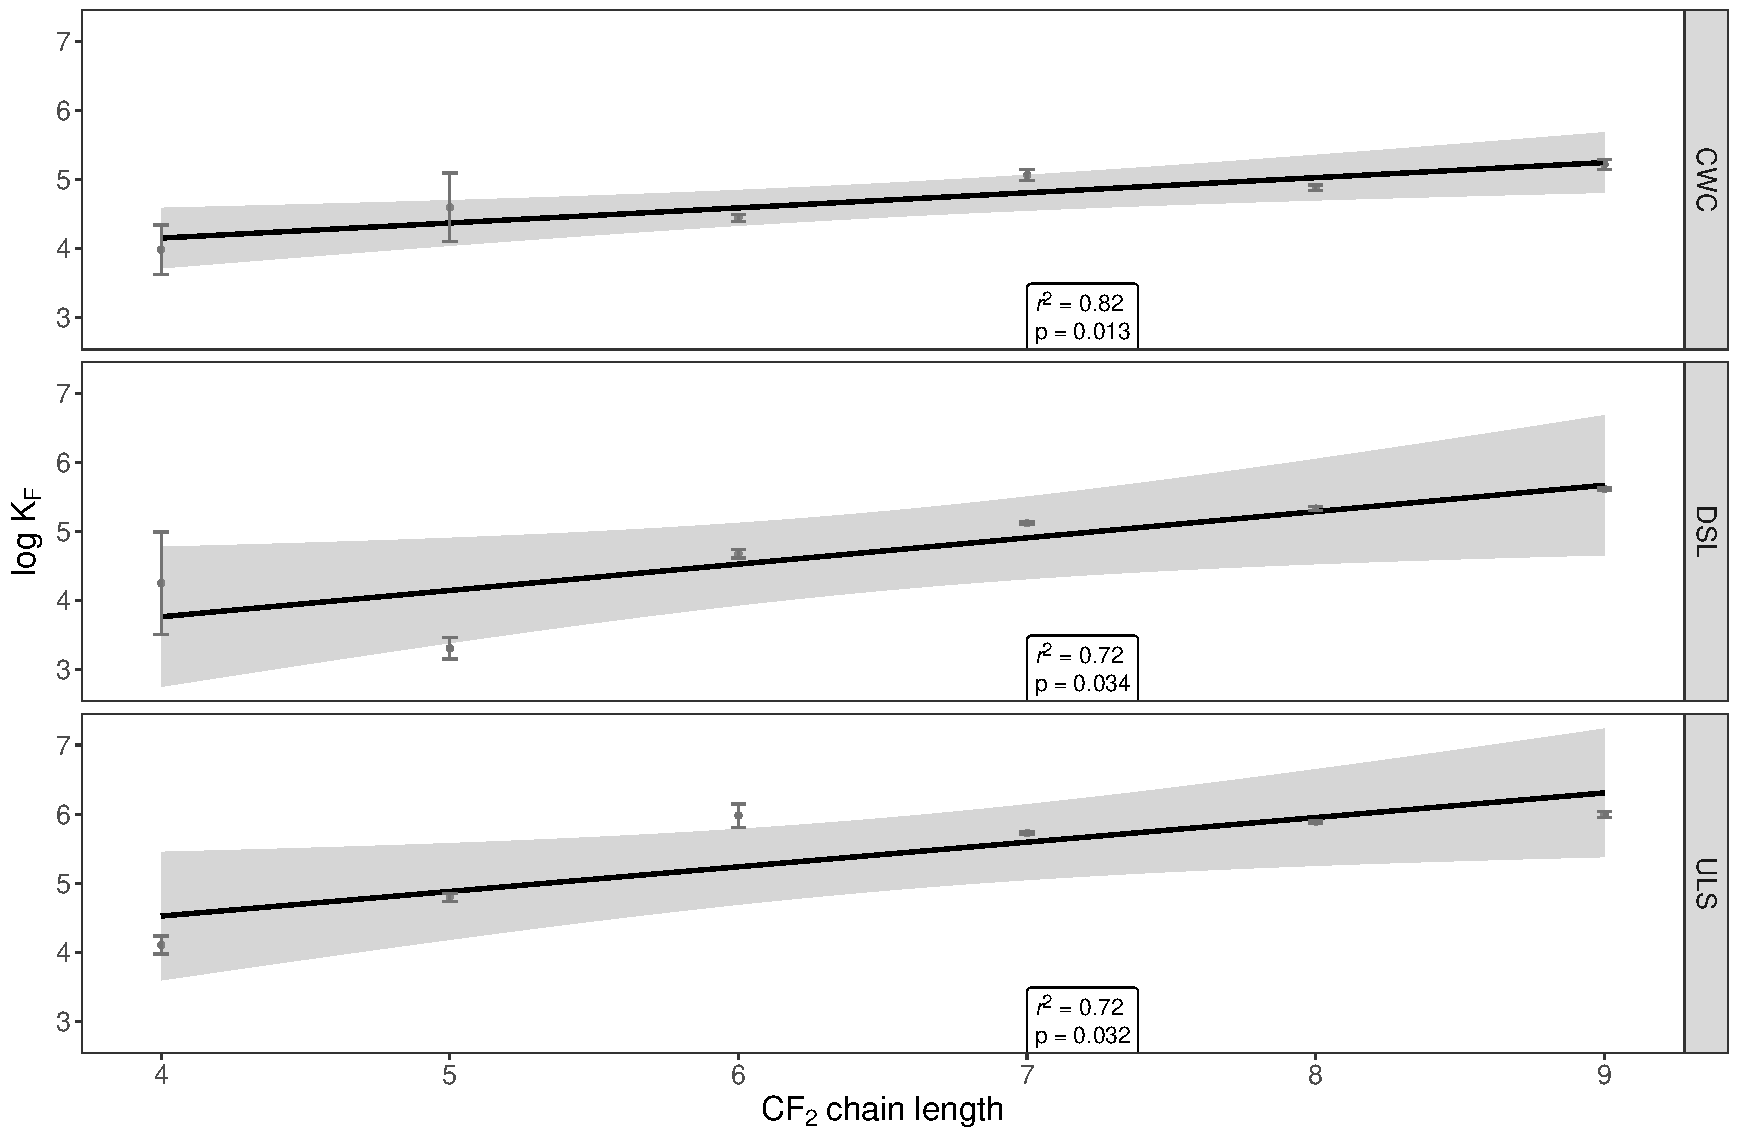
\includegraphics[width=0.7\textwidth]{R/figs/chainlength_KF.pdf}
    \caption{Correlation plot of $log~K_F$ as a function of PFCA chain length (number of $CF_2$ moieties) for the different biochars fitted by linear regression. The error bars and gray area represent the standard error for each $log~K_F$ and the regression line, respectively (n=9).}
    \label{fig:chainlength}
\end{figure}

\begin{figure*}[t!]
    \centering
    \begin{subfigure}[t]{0.5\textwidth}
        \centering
        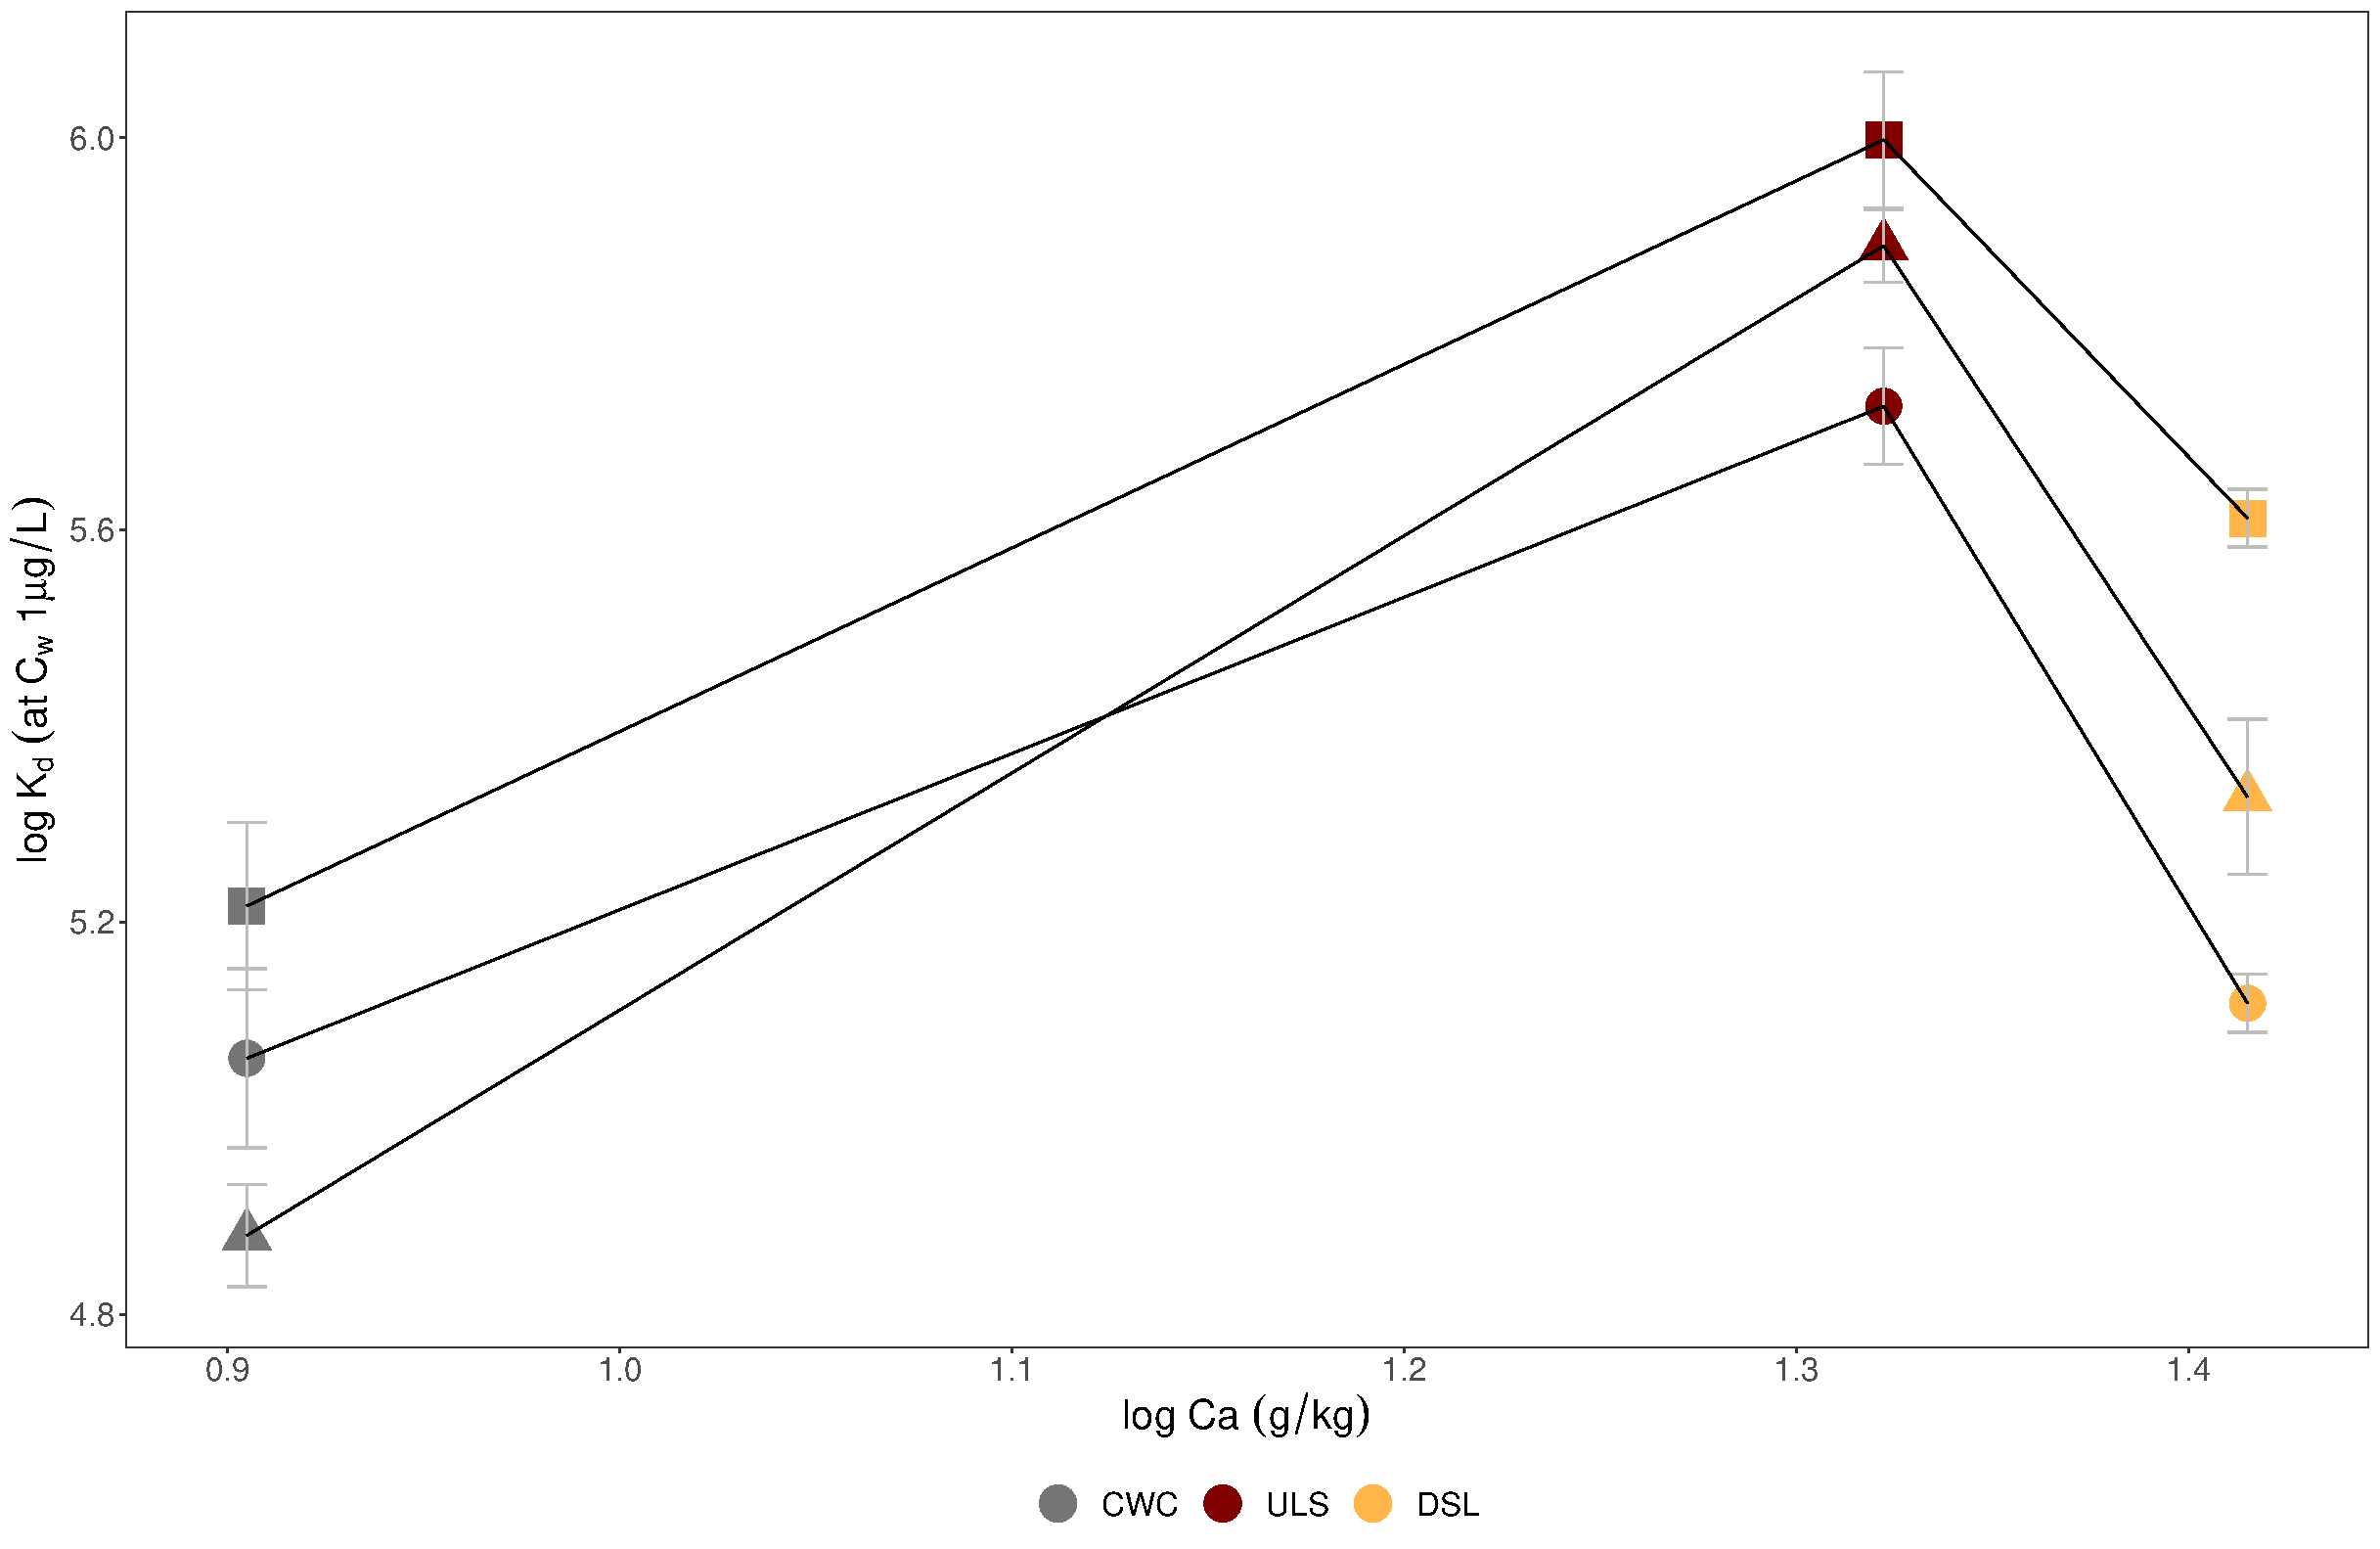
\includegraphics[height=6cm]{R/figs/Kd_1ugL_Ca.pdf}
        \caption{}
        \label{subfig:Ca}
    \end{subfigure}%
    ~ 
    \begin{subfigure}[t]{0.5\textwidth}
        \centering
        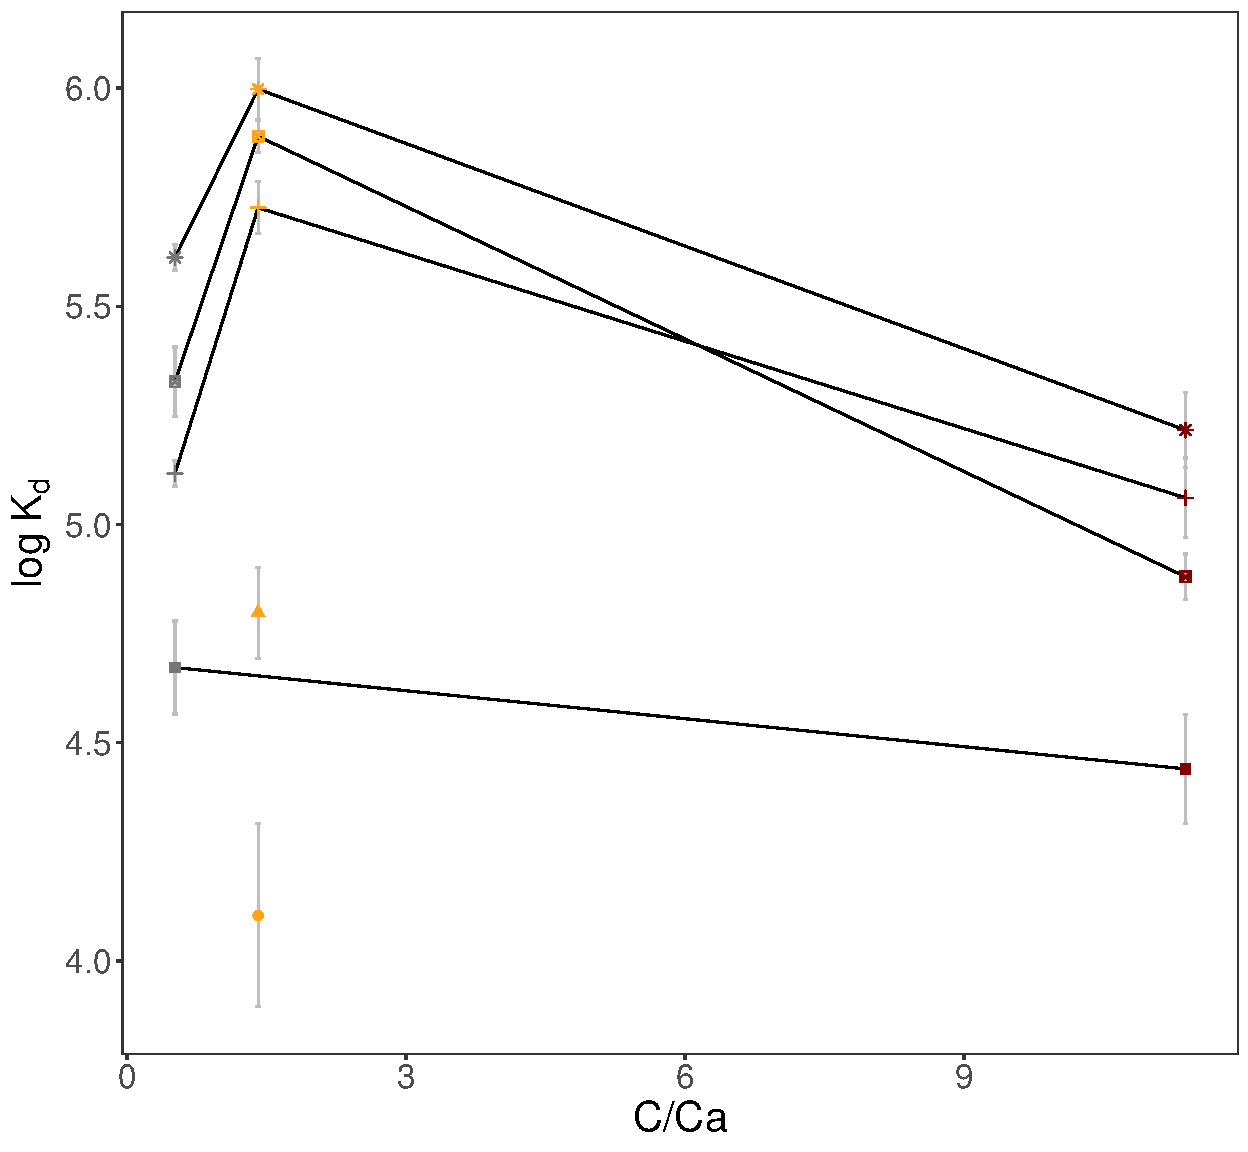
\includegraphics[height=6cm]{R/figs/Kd_1ugL_C_Ca.pdf}
        \caption{}
        \label{subfig:C_Ca}
    \end{subfigure}
    \medskip
    \begin{subfigure}[t]{0.5\textwidth}
        \centering
        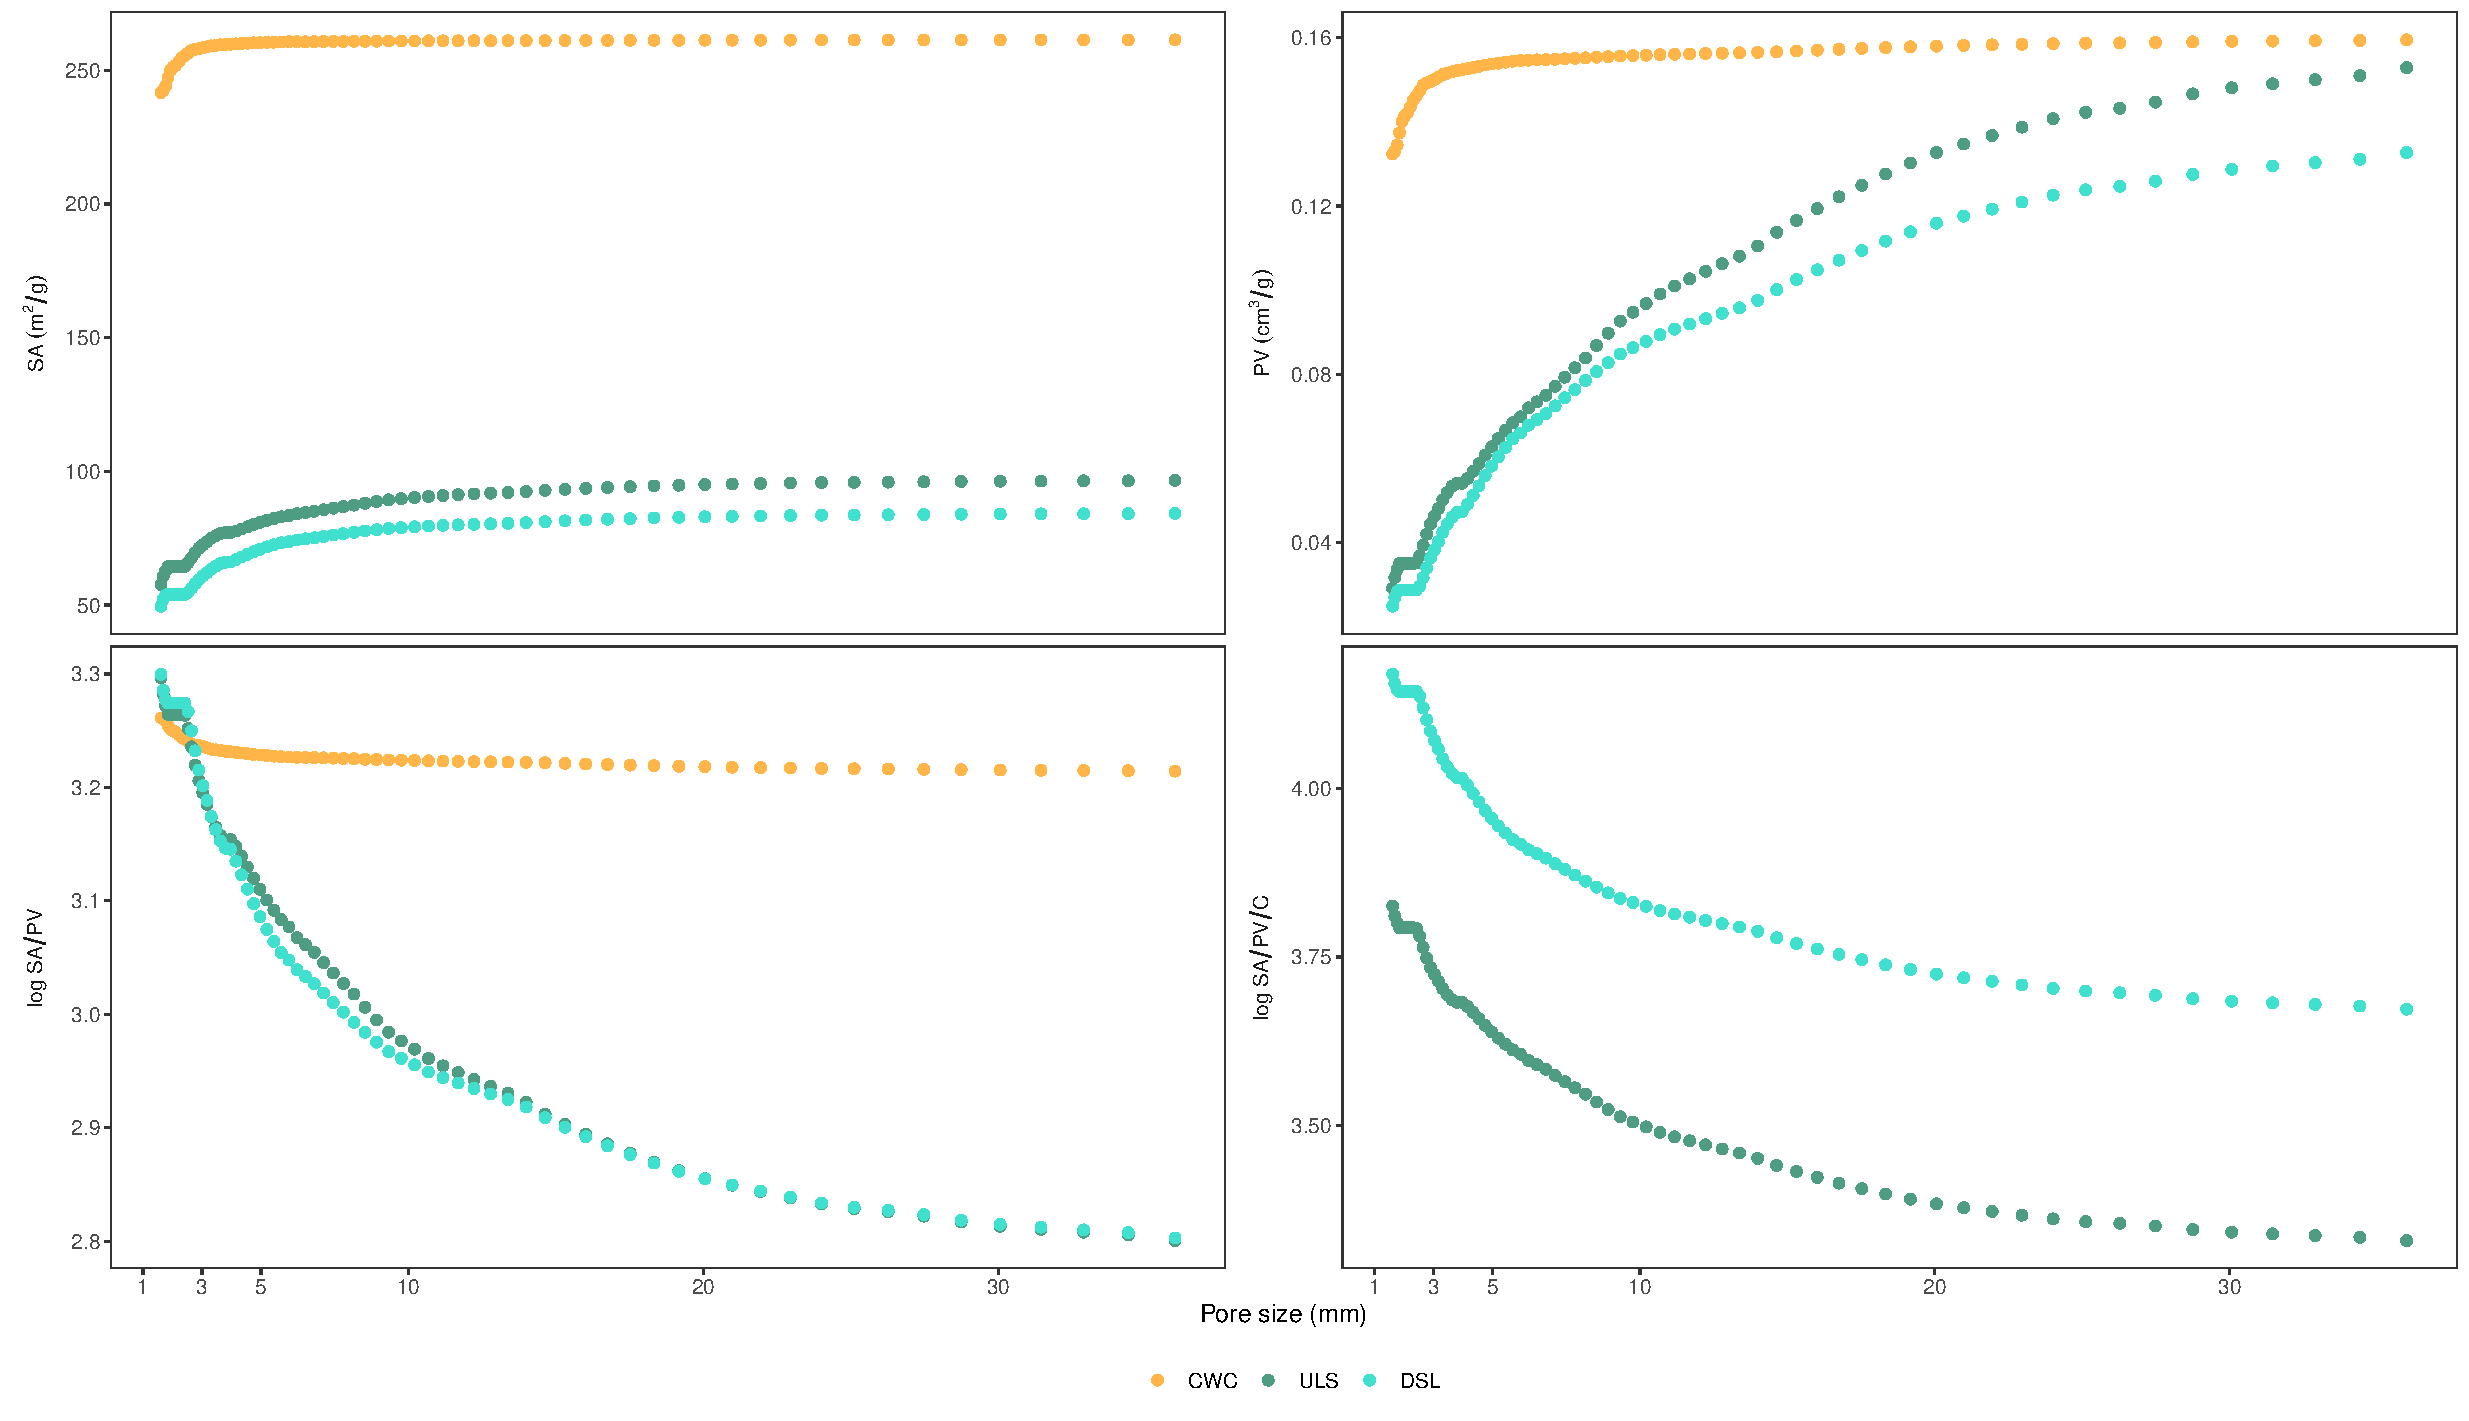
\includegraphics[height=6cm]{R/figs/Kd_1ugL_Fe.pdf}
        \caption{}
        \label{subfig:Fe}
    \end{subfigure}%
    ~ 
    \begin{subfigure}[t]{0.5\textwidth}
        \centering
        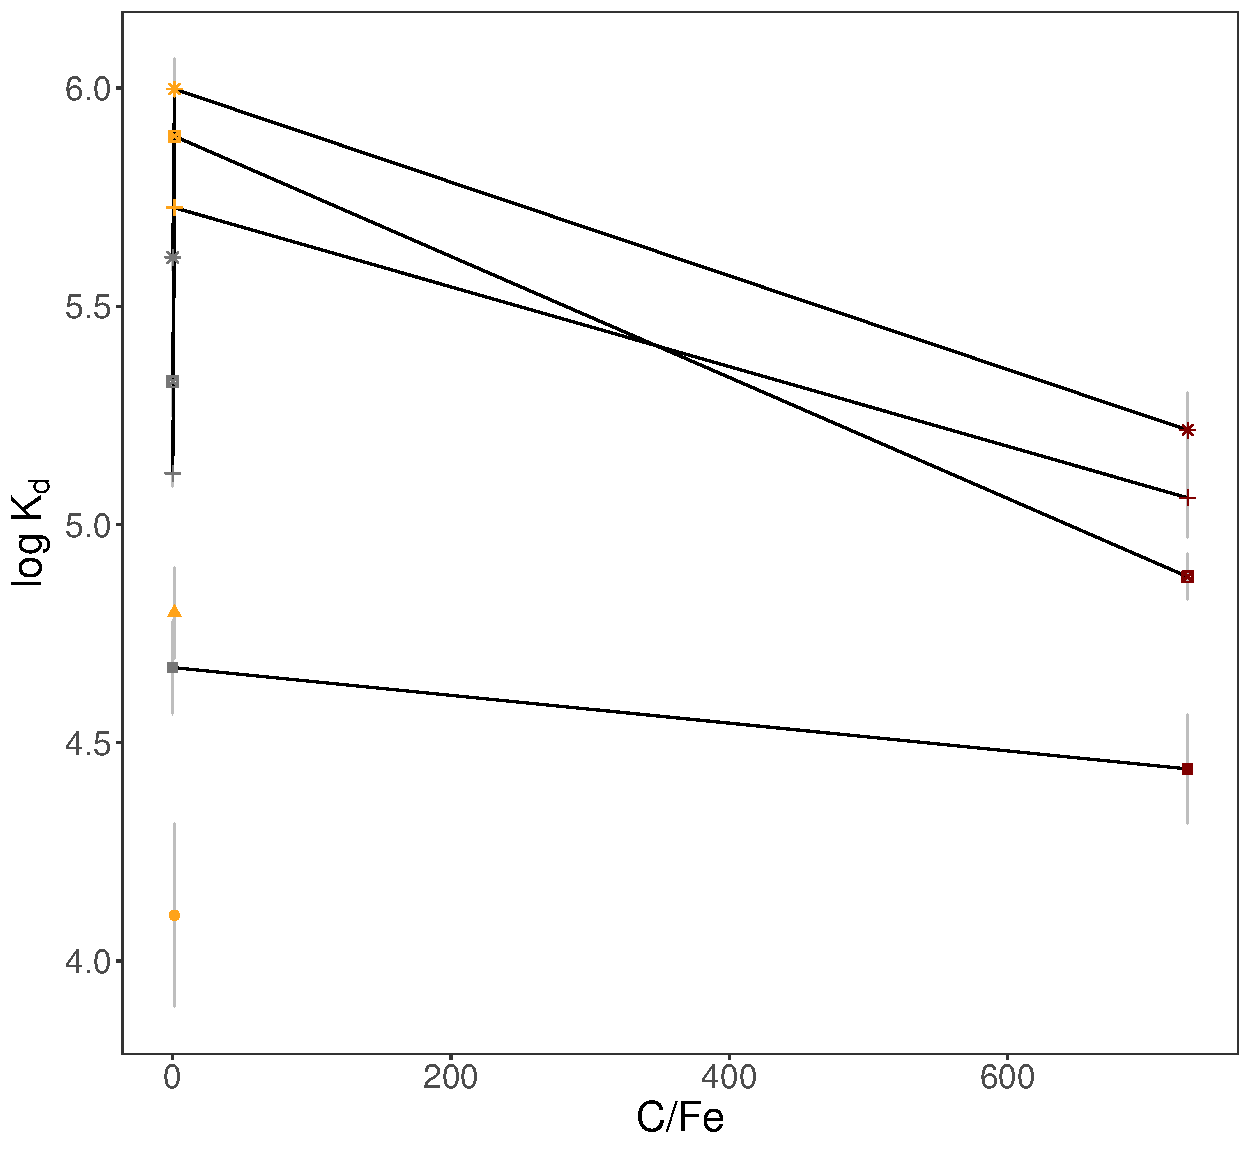
\includegraphics[height=6cm]{R/figs/Kd_1ugL_C_Fe.pdf}
        \caption{}
        \label{subfig:C_Fe}
    \end{subfigure}
    \label{fig:C_Ca_Fe}
    \caption{}
\end{figure*}

\begin{table}
\centering
\caption{Correlation table $log~K_d$ normalized to 1 \textmu g L\textsuperscript{-1} $C_w$.}
\label{tab:correlation}
\adjustbox{max width=\textwidth}{
\begin{tabular}{lrrrrrrrrrrrrrrrrrr} \toprule
PFCA & \multicolumn{2}{c}{Ca} & \multicolumn{2}{c}{Fe} & \multicolumn{2}{c}{C} & \multicolumn{2}{c}{C/Ca} & \multicolumn{2}{c}{C/Fe} & \multicolumn{2}{c}{SA small} & \multicolumn{2}{c}{PV small} & \multicolumn{2}{c}{SA large} & \multicolumn{2}{c}{PV large} \\ \cmidrule(l){2-3} \cmidrule(l){4-5} \cmidrule(l){6-7} \cmidrule(l){8-9} \cmidrule(l){10-11} \cmidrule(l){12-13} \cmidrule(l){14-15} \cmidrule(l){16-17} \cmidrule(l){18-19}
 & \multicolumn{1}{c}{$r^2$} & \multicolumn{1}{c}{$p$} & \multicolumn{1}{c}{$r^2$} & \multicolumn{1}{c}{$p$} & \multicolumn{1}{c}{$r^2$} & \multicolumn{1}{c}{$p$} & \multicolumn{1}{c}{$r^2$} & \multicolumn{1}{c}{$p$} & \multicolumn{1}{c}{$r^2$} & \multicolumn{1}{c}{$p$} & \multicolumn{1}{c}{$r^2$} & \multicolumn{1}{c}{$p$} & \multicolumn{1}{c}{$r^2$} & \multicolumn{1}{c}{$p$} & \multicolumn{1}{c}{$r^2$} & \multicolumn{1}{c}{$p$} & \multicolumn{1}{c}{$r^2$} & \multicolumn{1}{c}{$p$} \\ \midrule
PFPeA & 0.92 & 0.19 & 0.87 & 0.23 & 0.87 & 0.23 & 0.77 & 0.31 & 0.71 & 0.36 & 0.81 & 0.28 & 0.81 & 0.29 & 0.78 & 0.31 & 0.59 & 0.44 \\
PFHxA & 0.1 & 0.79 & 0.1 & 0.79 & 0.15 & 0.74 & 0.25 & 0.66 & 0.32 & 0.62 & 0.21 & 0.69 & 0.22 & 0.69 & 0.25 & 0.67 & 0.44 & 0.54 \\
PFHpA & 0.15 & 0.75 & 0.069 & 0.83 & 0.2 & 0.7 & 0.31 & 0.62 & 0.38 & 0.58 & 0.27 & 0.65 & 0.27 & 0.65 & 0.31 & 0.63 & 0.51 & 0.5 \\
PFOA & 0.1 & 0.79 & 0.11 & 0.79 & 0.15 & 0.74 & 0.25 & 0.67 & 0.32 & 0.62 & 0.21 & 0.7 & 0.22 & 0.69 & 0.25 & 0.67 & 0.44 & 0.54 \\
PFNA & 0.42 & 0.55 & 0.0026 & 0.97 & 0.5 & 0.5 & 0.62 & 0.42 & 0.69 & 0.38 & 0.58 & 0.45 & 0.58 & 0.45 & 0.62 & 0.42 & 0.8 & 0.29 \\
PFDA & 0.5 & 0.5 & 0.015 & 0.92 & 0.57 & 0.45 & 0.69 & 0.38 & 0.75 & 0.33 & 0.65 & 0.41 & 0.65 & 0.4 & 0.69 & 0.38 & 0.86 & 0.25 \\
 &  &  &  &  &  &  &  &  &  &  &  &  &  &  &  &  &  &  \\ \midrule
PFCA & \multicolumn{2}{c}{SA large/Fe} & \multicolumn{2}{c}{SA large/Ca} & \multicolumn{2}{c}{SA small/Fe} & \multicolumn{2}{c}{SA small/Ca} & \multicolumn{2}{c}{PV large/Fe} & \multicolumn{2}{c}{PV large/Ca} & \multicolumn{2}{c}{PV small/Fe} & \multicolumn{2}{c}{PV small/Ca} &  &  \\ \cmidrule(l){2-3} \cmidrule(l){4-5} \cmidrule(l){6-7} \cmidrule(l){8-9} \cmidrule(l){10-11} \cmidrule(l){12-13} \cmidrule(l){14-15} \cmidrule(l){16-17}
 & \multicolumn{1}{c}{$r^2$} & \multicolumn{1}{c}{$p$} & \multicolumn{1}{c}{$r^2$} & \multicolumn{1}{c}{$p$} & \multicolumn{1}{c}{$r^2$} & \multicolumn{1}{c}{$p$} & \multicolumn{1}{c}{$r^2$} & \multicolumn{1}{c}{$p$} & \multicolumn{1}{c}{$r^2$} & \multicolumn{1}{c}{$p$} & \multicolumn{1}{c}{$r^2$} & \multicolumn{1}{c}{$p$} & \multicolumn{1}{c}{$r^2$} & \multicolumn{1}{c}{$p$} & \multicolumn{1}{c}{$r^2$} & \multicolumn{1}{c}{$p$} &  &  \\ \midrule
PFPeA & 0.71 & 0.36 & 0.75 & 0.33 & 0.71 & 0.36 & 0.75 & 0.33 & 0.74 & 0.34 & 0.27 & 0.65 & 0.71 & 0.36 & 0.75 & 0.33 &  &  \\
PFHxA & 0.32 & 0.62 & 0.28 & 0.65 & 0.32 & 0.62 & 0.27 & 0.65 & 0.29 & 0.64 & 0.76 & 0.32 & 0.32 & 0.62 & 0.28 & 0.65 &  &  \\
PFHpA & 0.38 & 0.58 & 0.34 & 0.61 & 0.38 & 0.58 & 0.33 & 0.61 & 0.35 & 0.6 & 0.81 & 0.28 & 0.38 & 0.58 & 0.33 & 0.61 &  &  \\
PFOA & 0.32 & 0.62 & 0.28 & 0.65 & 0.32 & 0.62 & 0.27 & 0.65 & 0.29 & 0.64 & 0.76 & 0.32 & 0.32 & 0.62 & 0.27 & 0.65 &  &  \\
PFNA & 0.69 & 0.38 & 0.65 & 0.41 & 0.69 & 0.38 & 0.65 & 0.41 & 0.66 & 0.4 & 0.98 & 0.082 & 0.69 & 0.38 & 0.65 & 0.41 &  &  \\
PFDA & 0.75 & 0.33 & 0.72 & 0.36 & 0.76 & 0.33 & 0.71 & 0.36 & 0.73 & 0.35 & 1 & 0.035 & 0.76 & 0.33 & 0.71 & 0.36 &  & \\ \bottomrule
\end{tabular}}
\end{table}

\begin{figure*}[t!]
    \centering
    \begin{subfigure}[t]{0.5\textwidth}
        \centering
        \includegraphics[height=5cm]{R/figs/Kd_1ugL_SAN2.pdf}
        \caption{}
        \label{subfig:SAN2}
    \end{subfigure}%
    ~ 
    \begin{subfigure}[t]{0.5\textwidth}
        \centering
        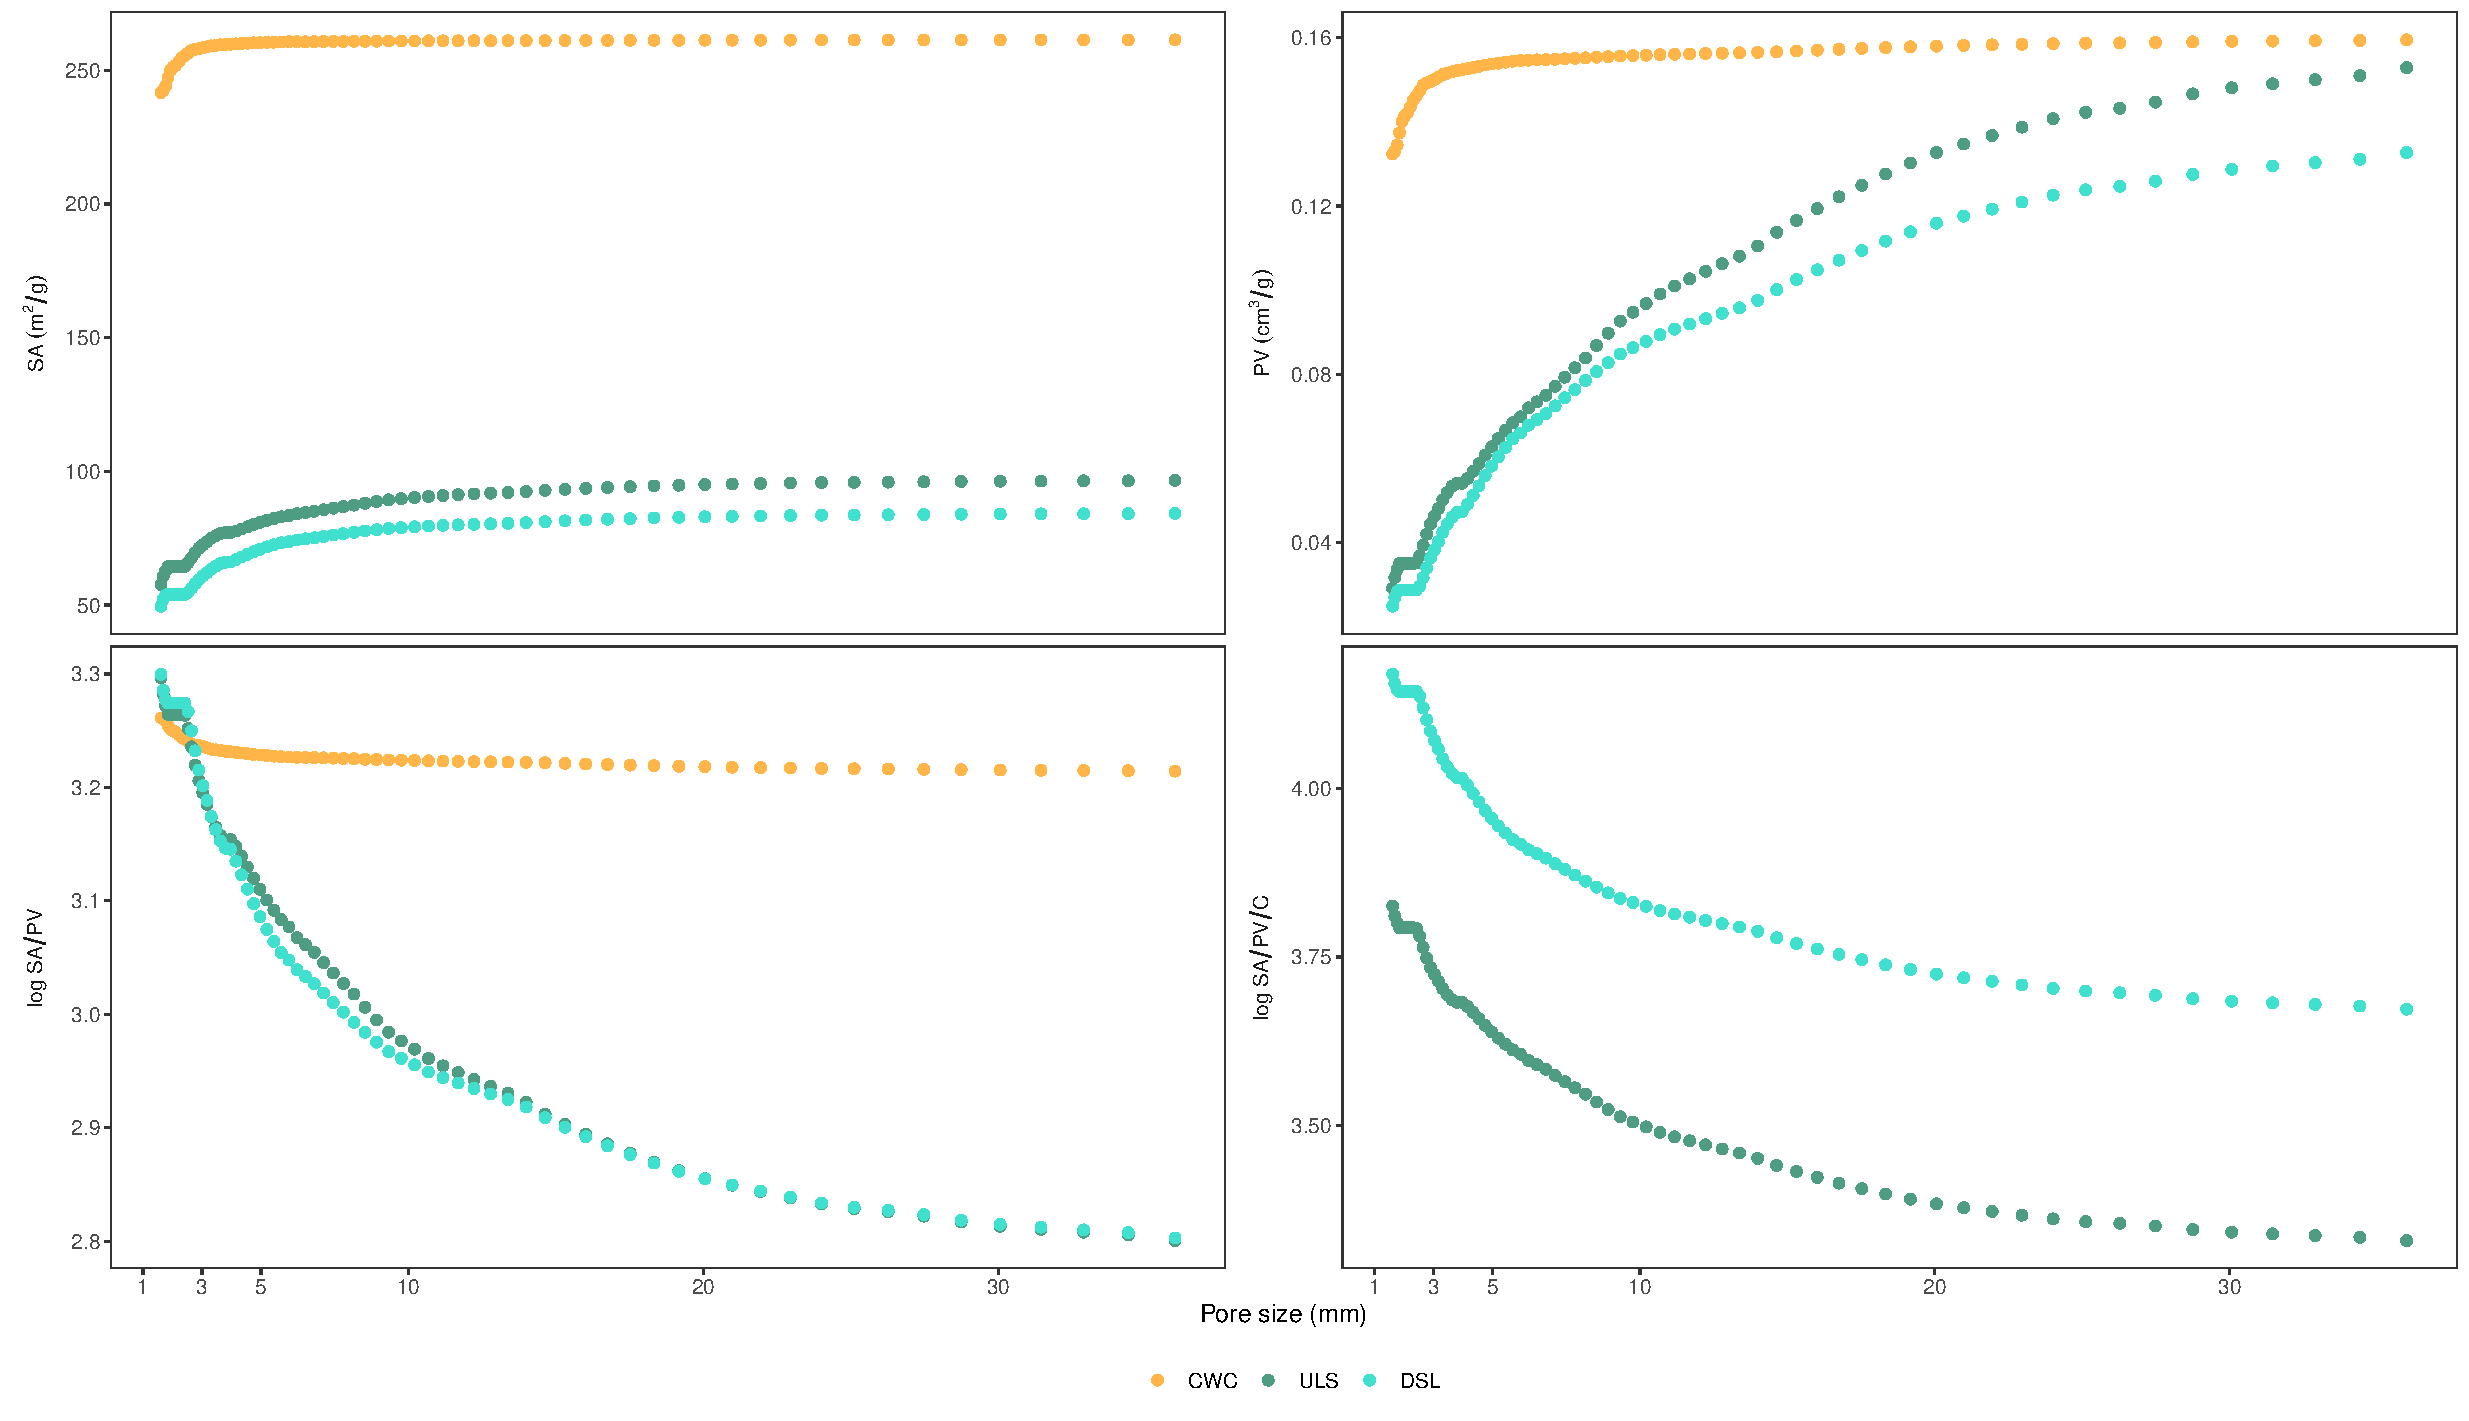
\includegraphics[height=5cm]{R/figs/Kd_1ugL_SACO2.pdf}
        \caption{}
        \label{subfig:SACO2}
    \end{subfigure}
    \medskip
    \begin{subfigure}[t]{0.5\textwidth}
        \centering
        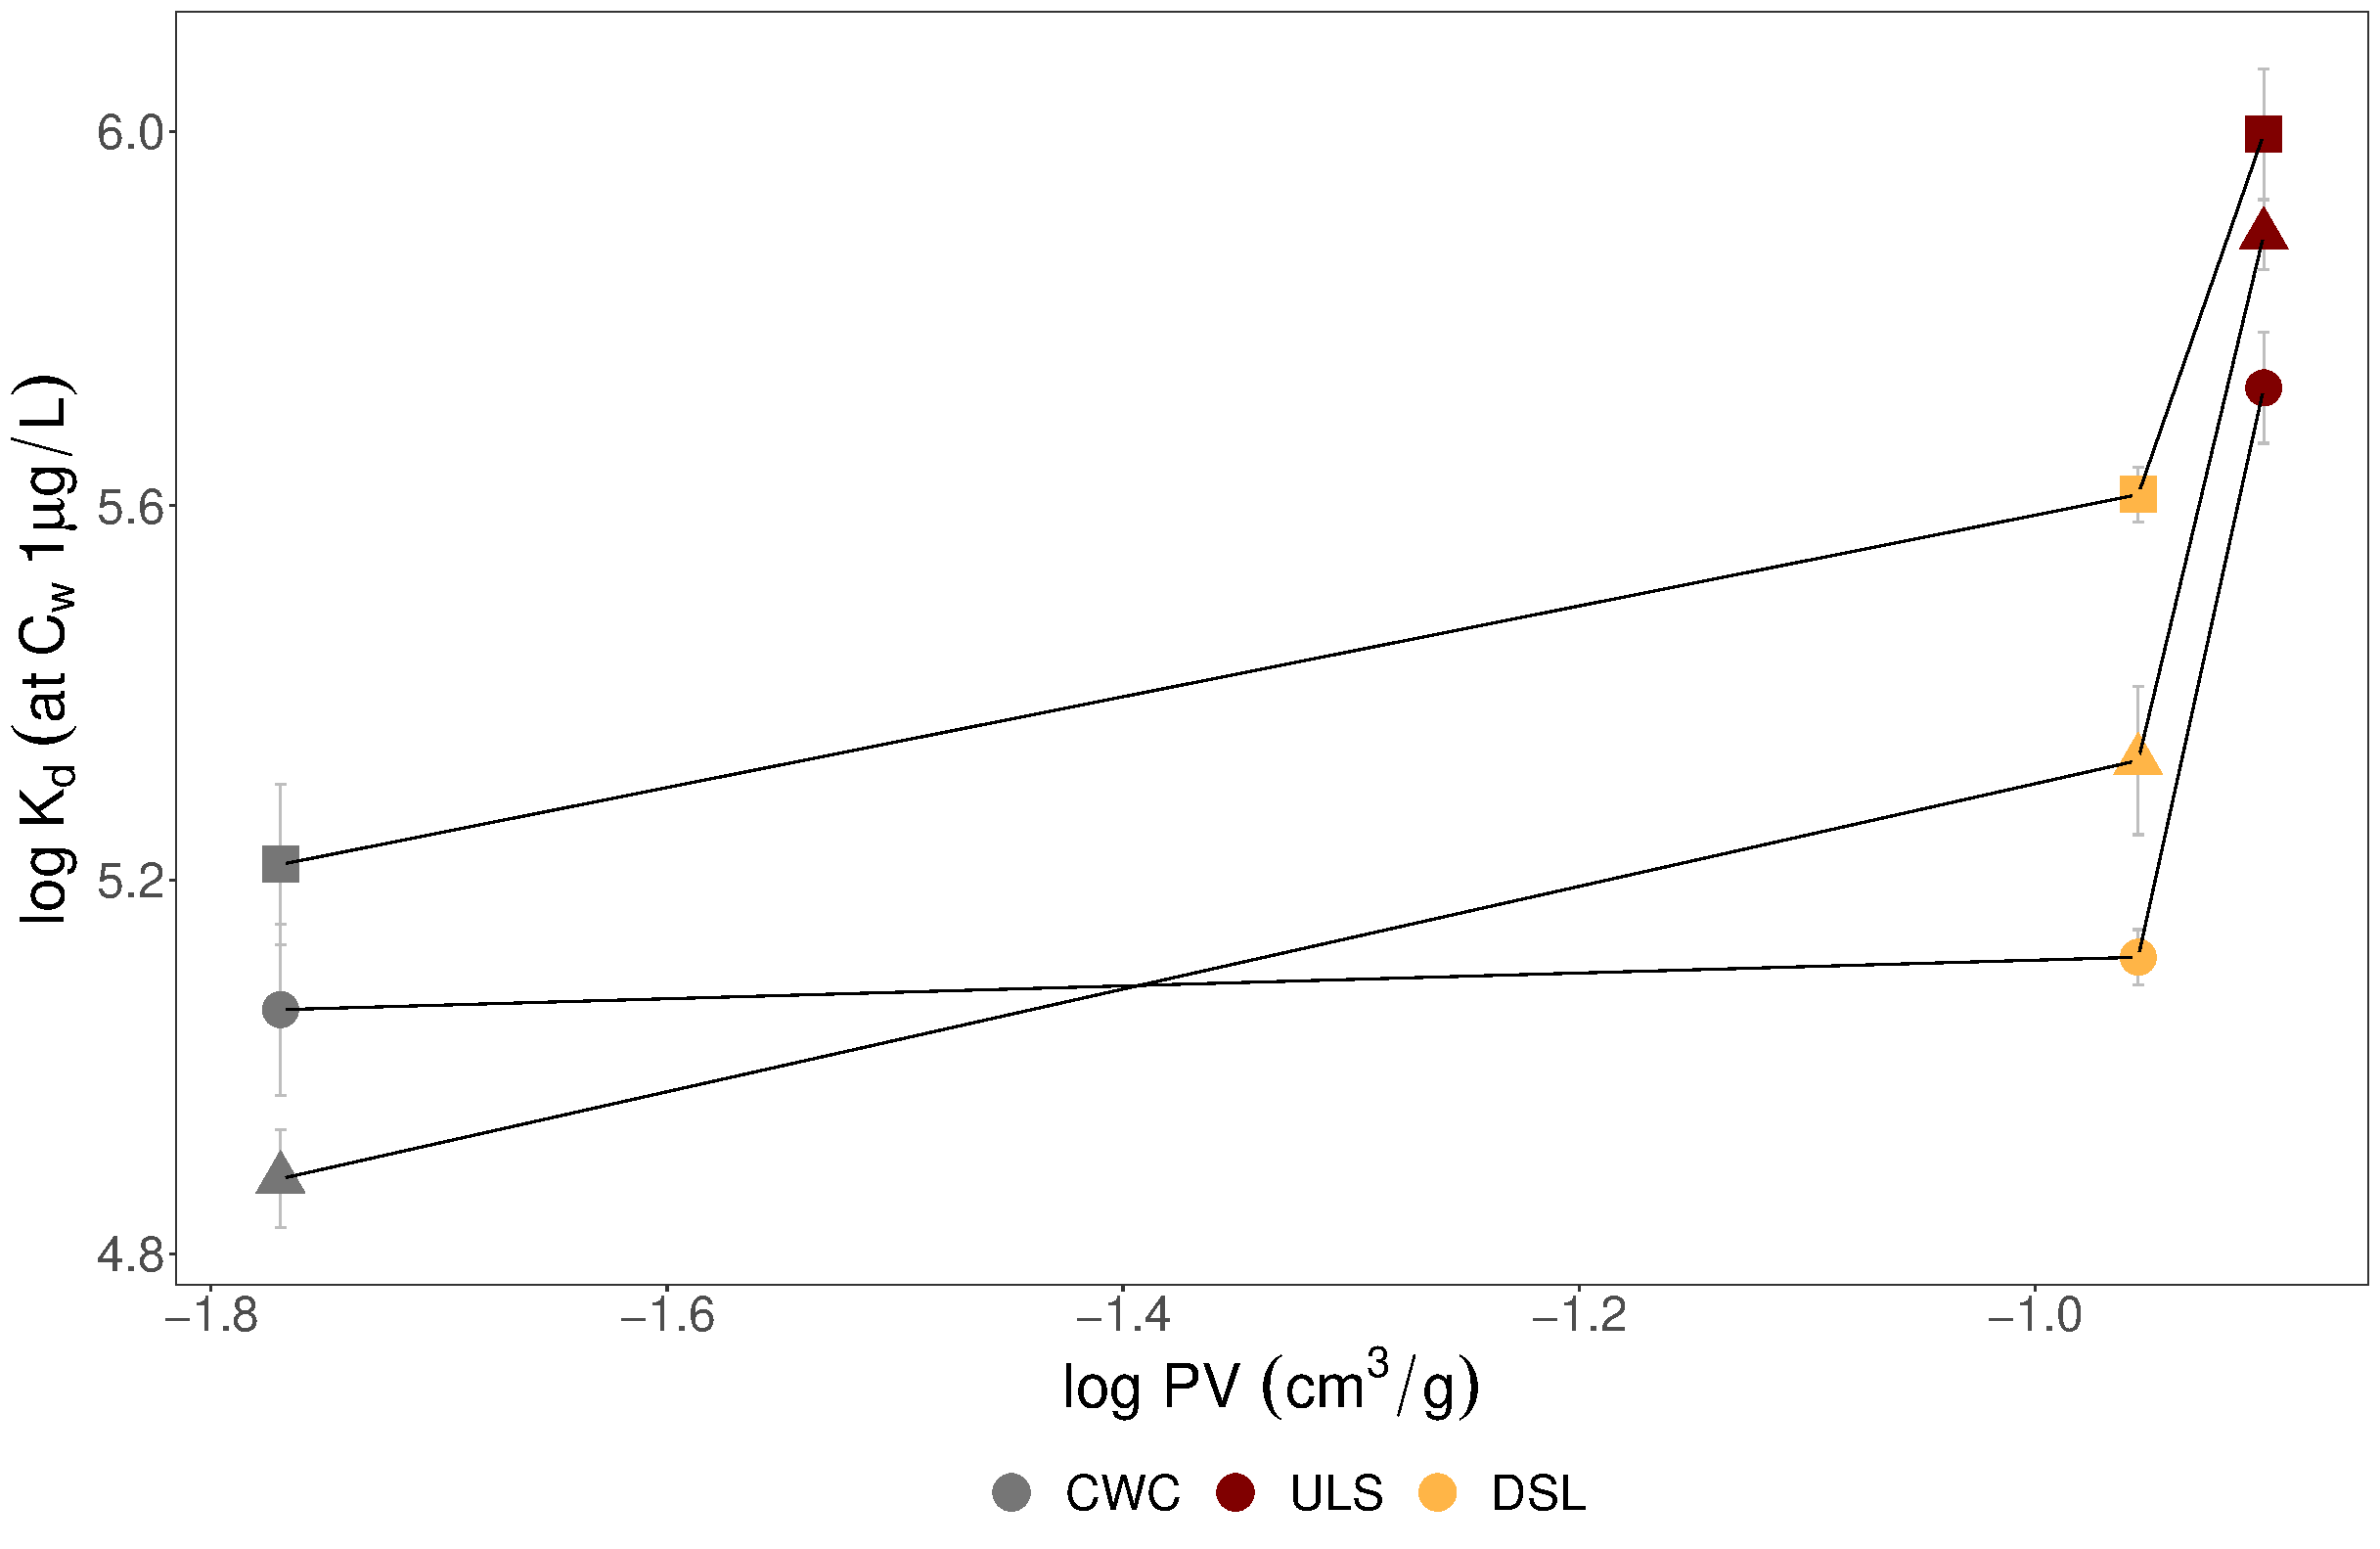
\includegraphics[height=5cm]{R/figs/Kd_1ugL_PVN2.pdf}
        \caption{}
        \label{subfig:PVN2}
    \end{subfigure}%
    ~ 
    \begin{subfigure}[t]{0.5\textwidth}
        \centering
        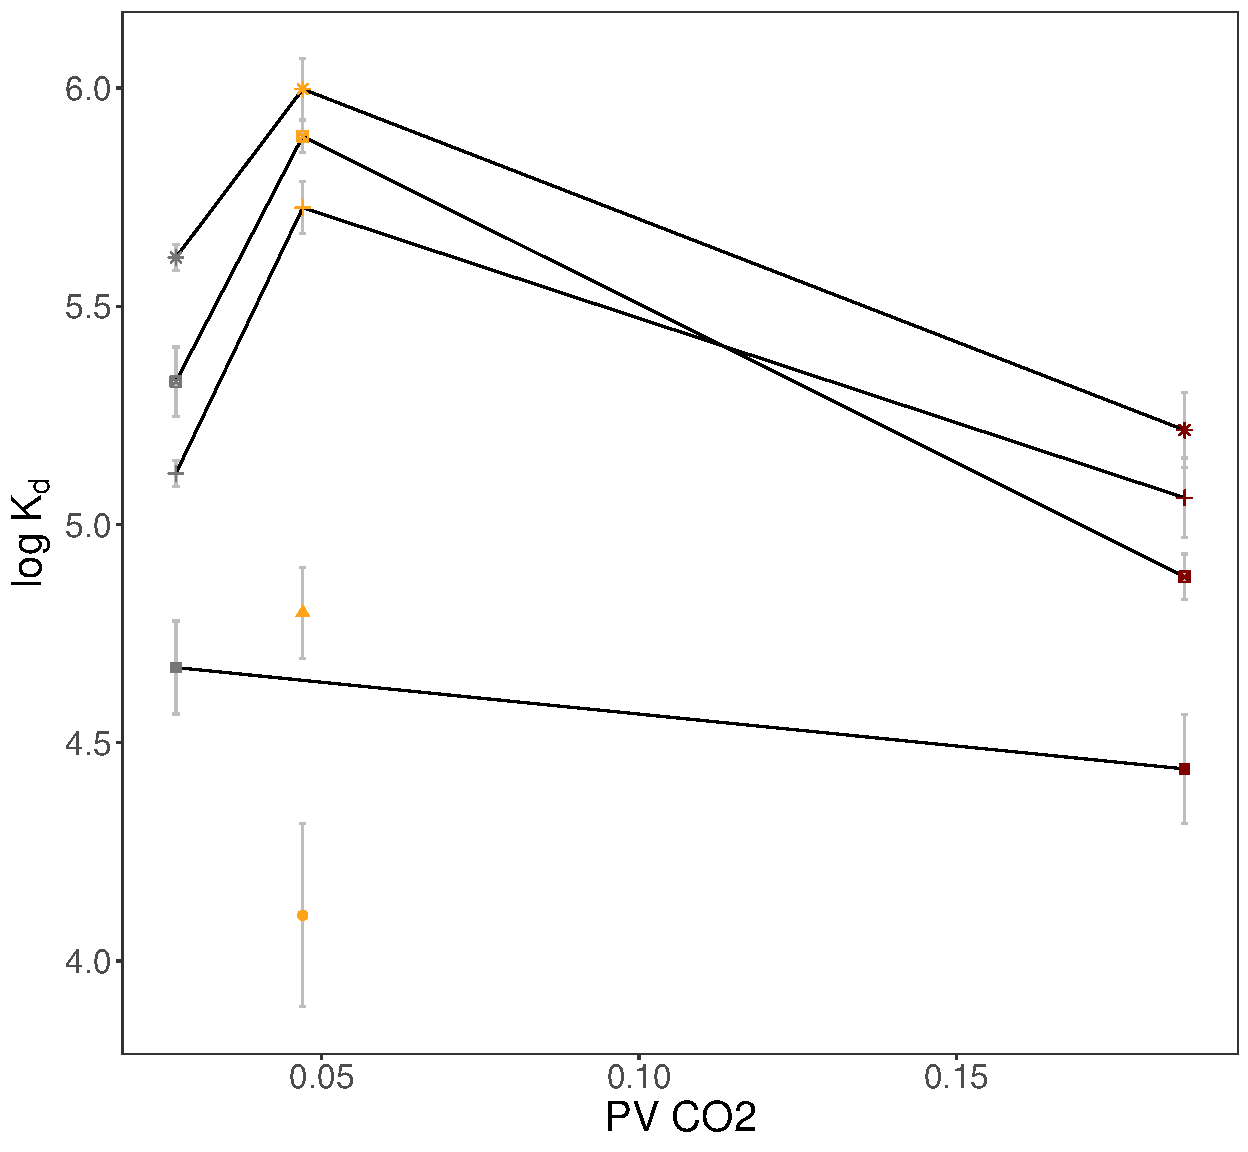
\includegraphics[height=5cm]{R/figs/Kd_1ugL_PVCO2.pdf}
        \caption{}
        \label{subfig:PVCO2}
    \end{subfigure}
    \medskip
    \begin{subfigure}[t]{0.5\textwidth}
        \centering
        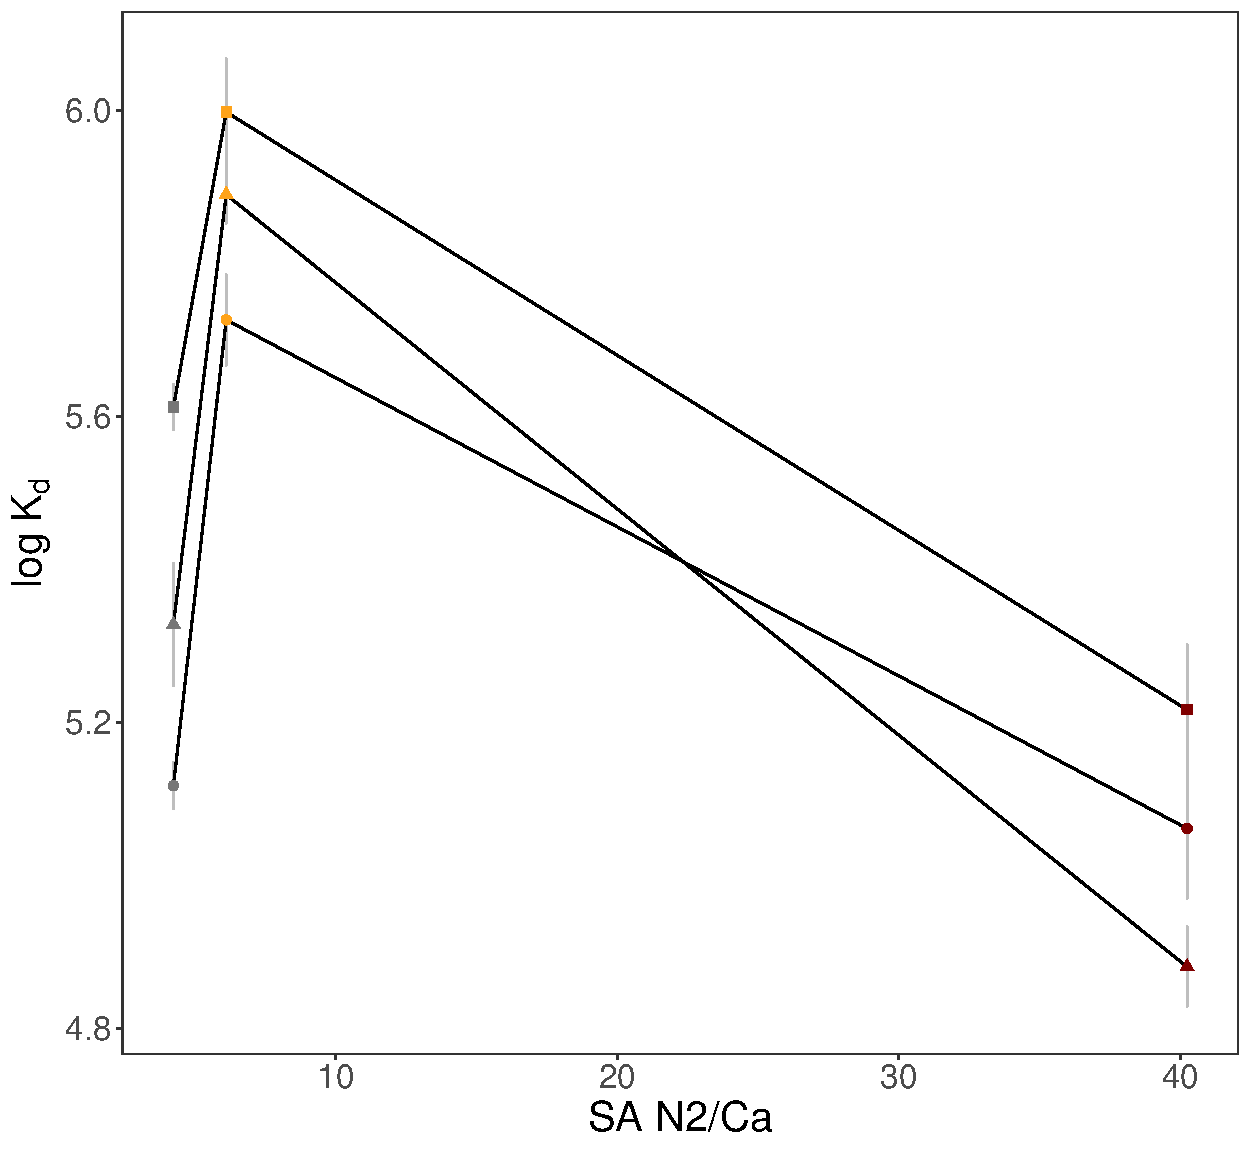
\includegraphics[height=5cm]{R/figs/Kd_1ugL_SAN2_Ca.pdf}
        \caption{}
        \label{subfig:SAN2_Ca}
    \end{subfigure}%
    ~ 
    \begin{subfigure}[t]{0.5\textwidth}
        \centering
        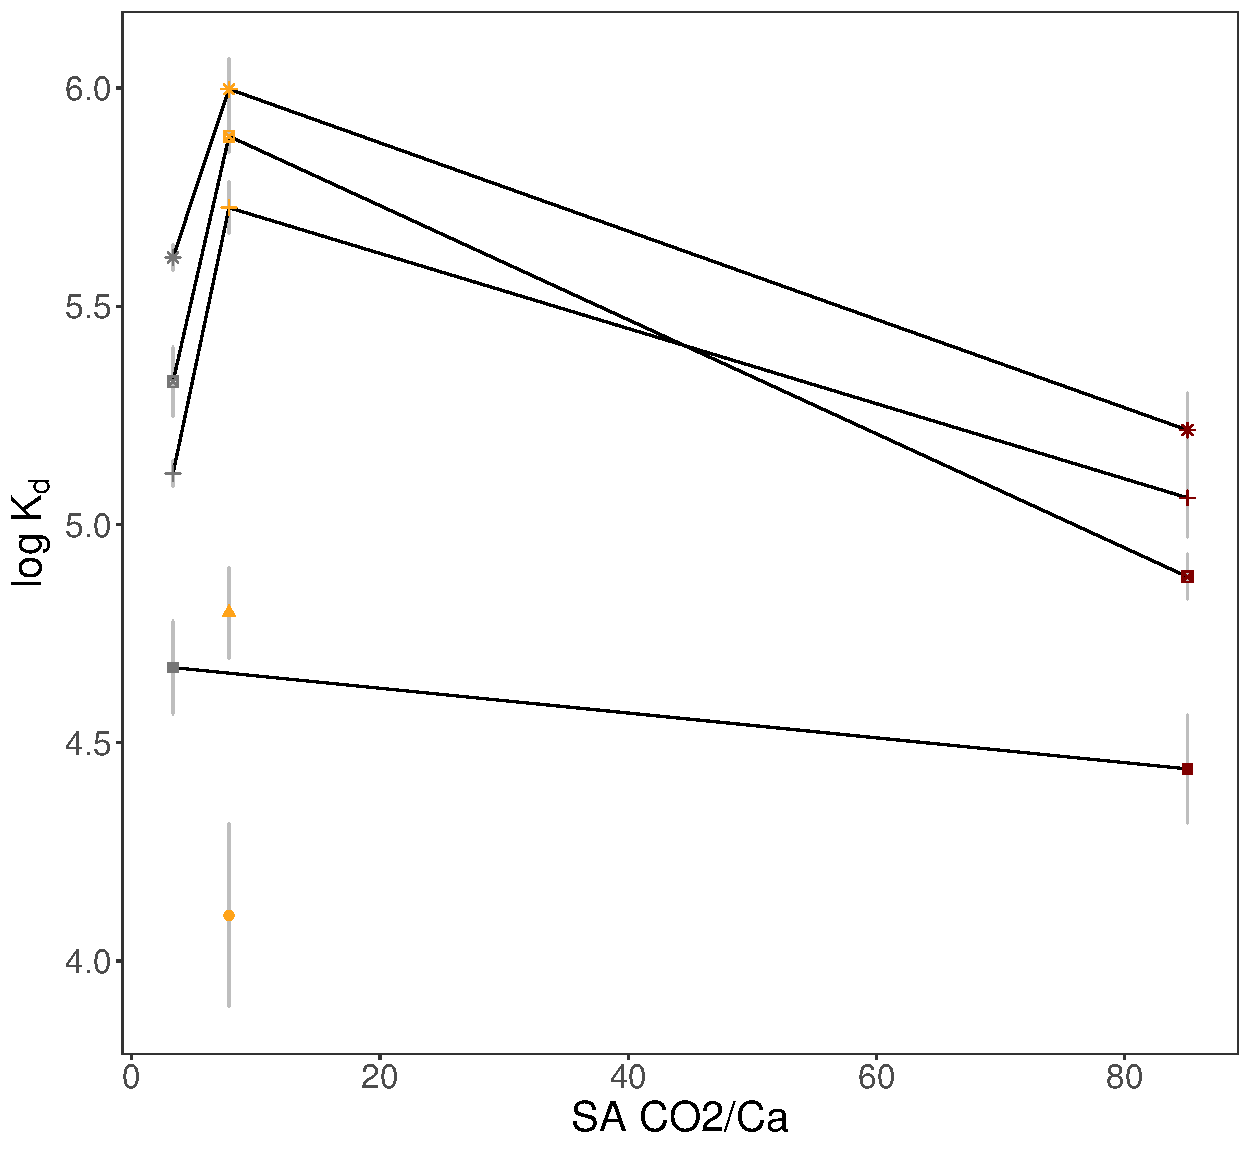
\includegraphics[height=5cm]{R/figs/Kd_1ugL_SACO2_Ca.pdf}
        \caption{}
        \label{subfig:SACO2_Ca}
    \end{subfigure}
    \medskip
    \begin{subfigure}[t]{0.5\textwidth}
        \centering
        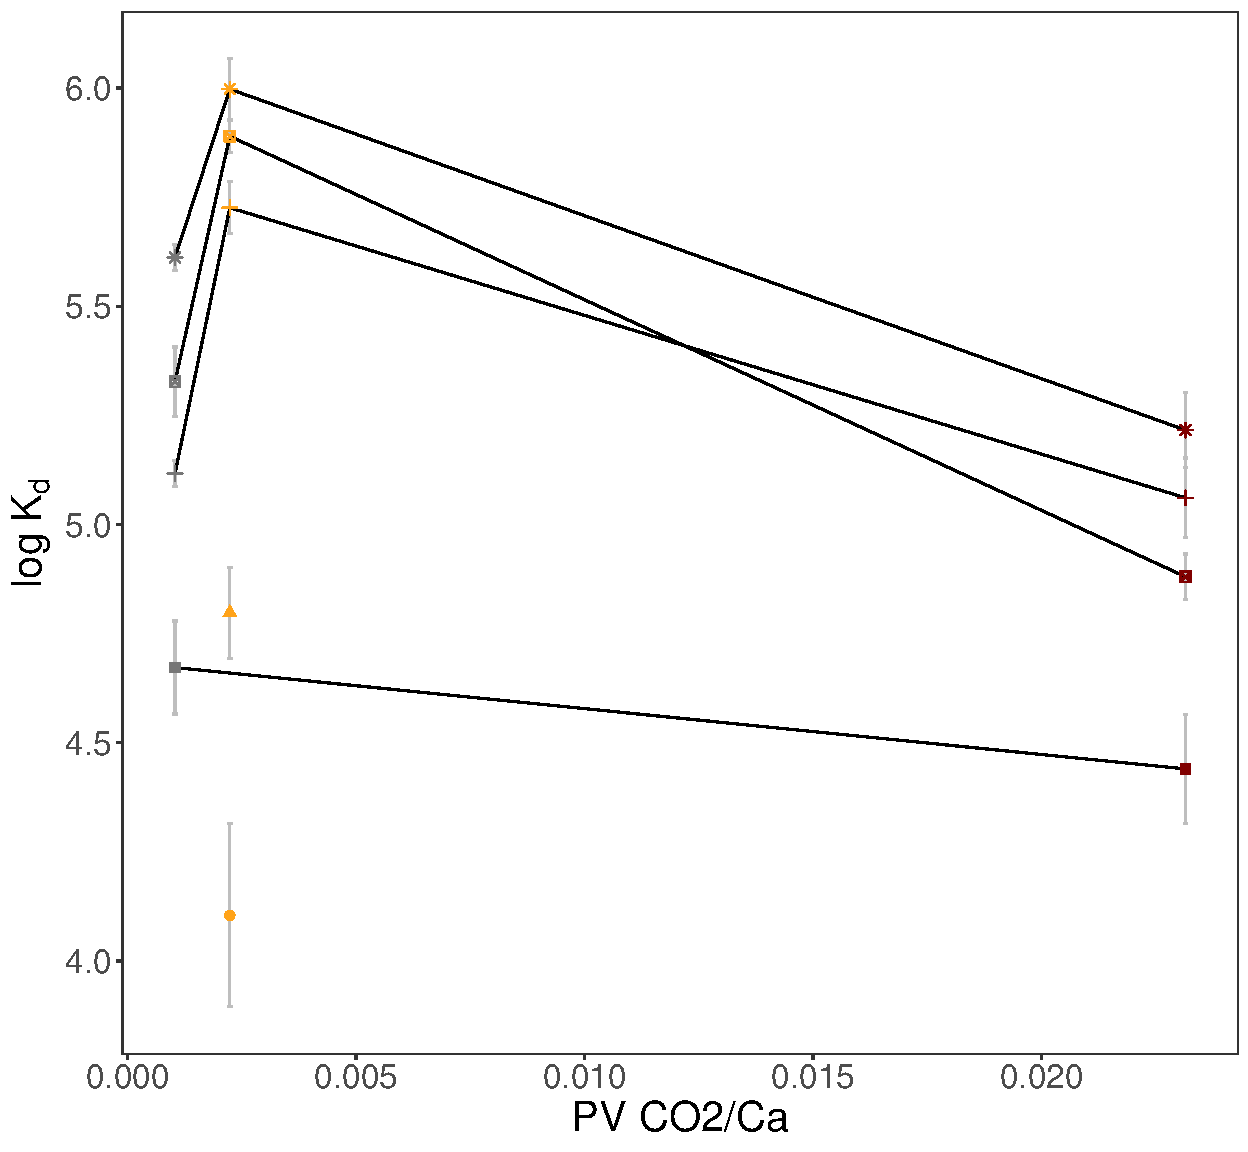
\includegraphics[height=5cm]{R/figs/Kd_1ugL_PVCO2_Ca.pdf}
        \caption{}
        \label{subfig:PVCO2_Ca}
    \end{subfigure}%
    ~ 
    \begin{subfigure}[t]{0.5\textwidth}
        \centering
        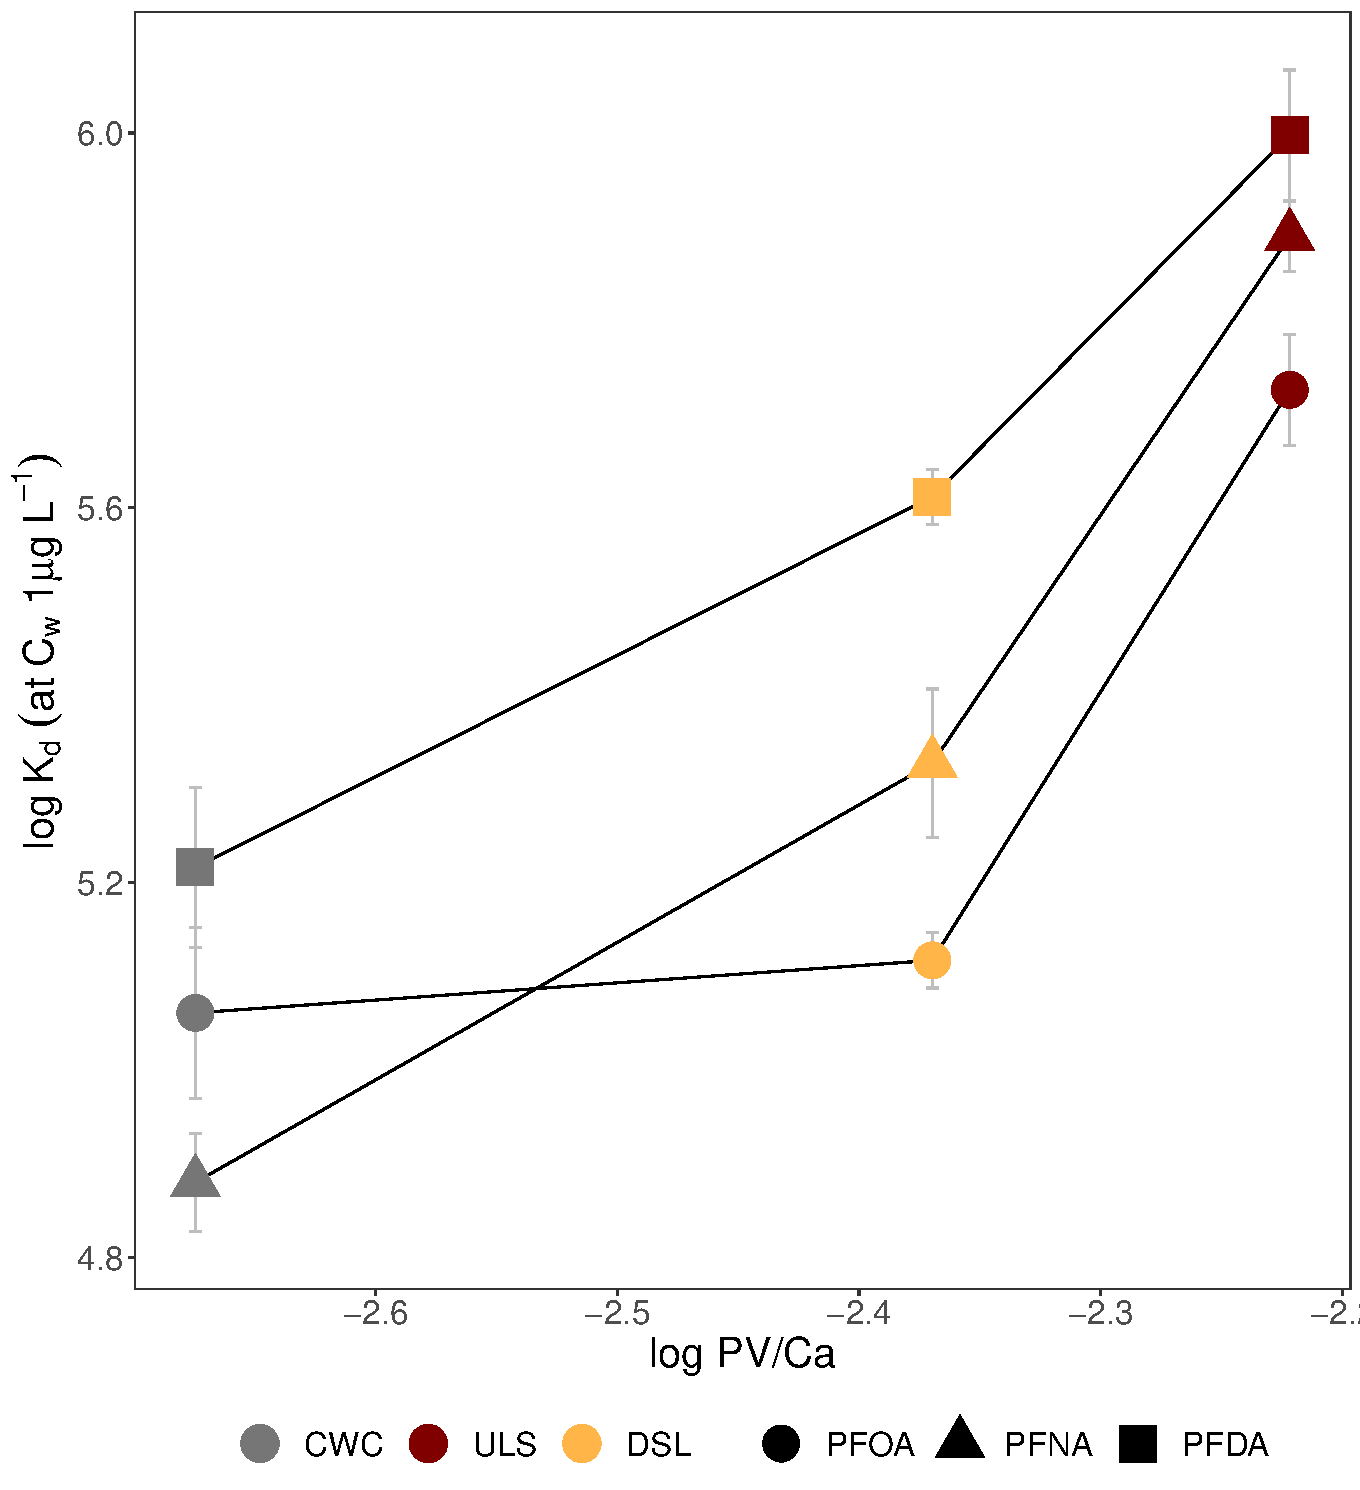
\includegraphics[height=5cm]{R/figs/Kd_1ugL_PVN2_Ca.pdf}
        \caption{}
        \label{subfig:PVN2_Ca}
    \end{subfigure}
\end{figure*}
\begin{figure*}[t]\ContinuedFloat
    \begin{subfigure}[t]{0.5\textwidth}
        \centering
        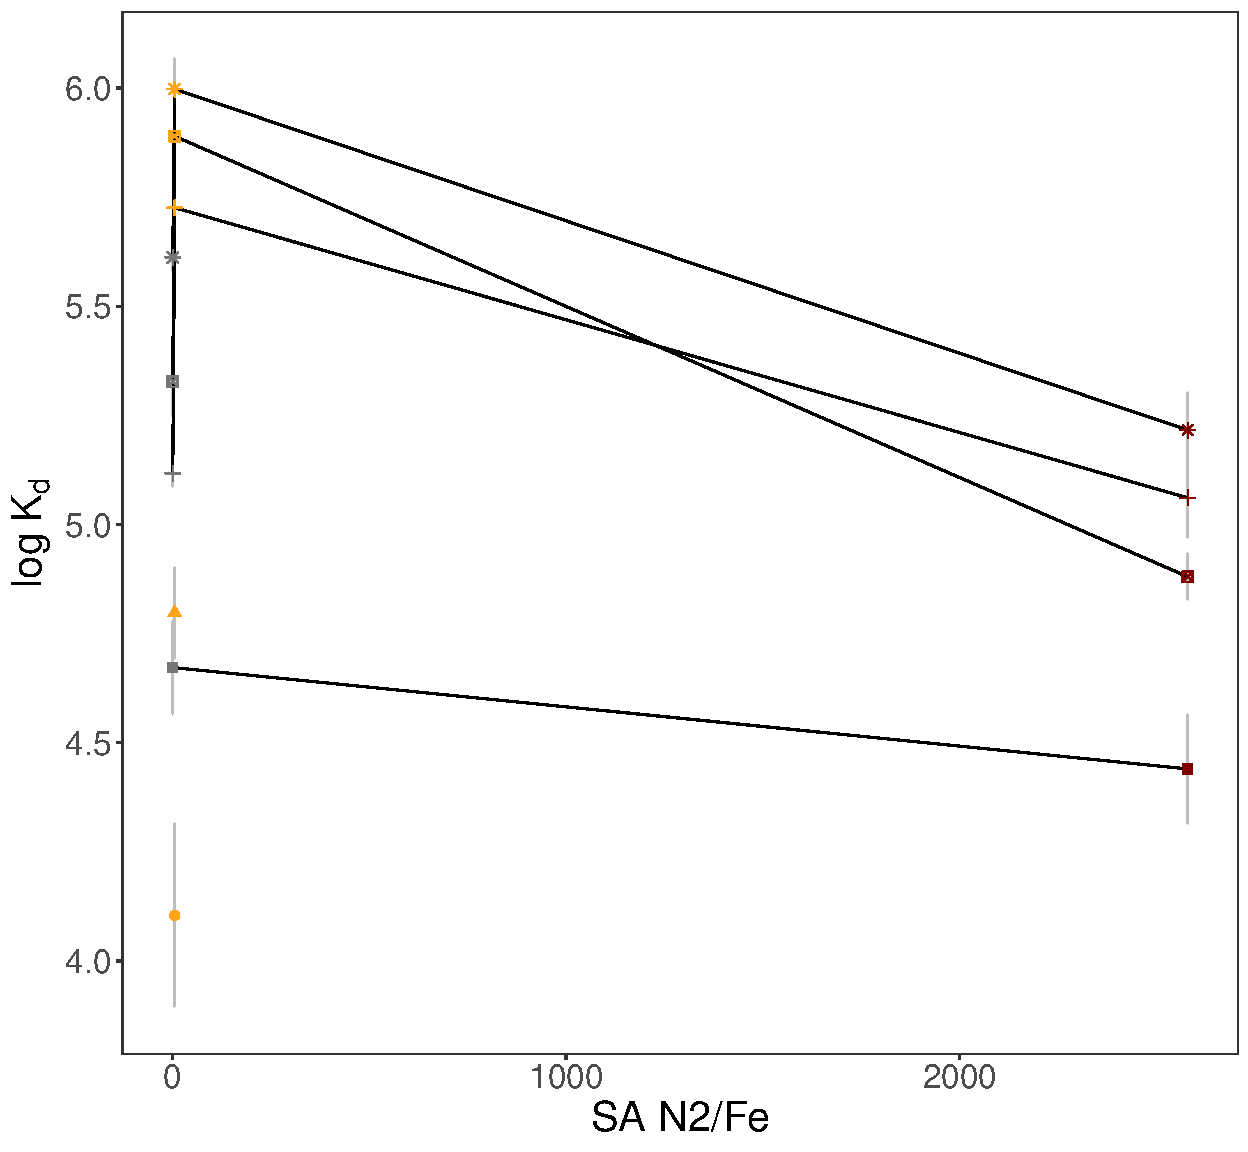
\includegraphics[height=5cm]{R/figs/Kd_1ugL_SAN2_Fe.pdf}
        \caption{}
        \label{subfig:SAN2_Fe}
    \end{subfigure}%
    ~ 
    \begin{subfigure}[t]{0.5\textwidth}
        \centering
        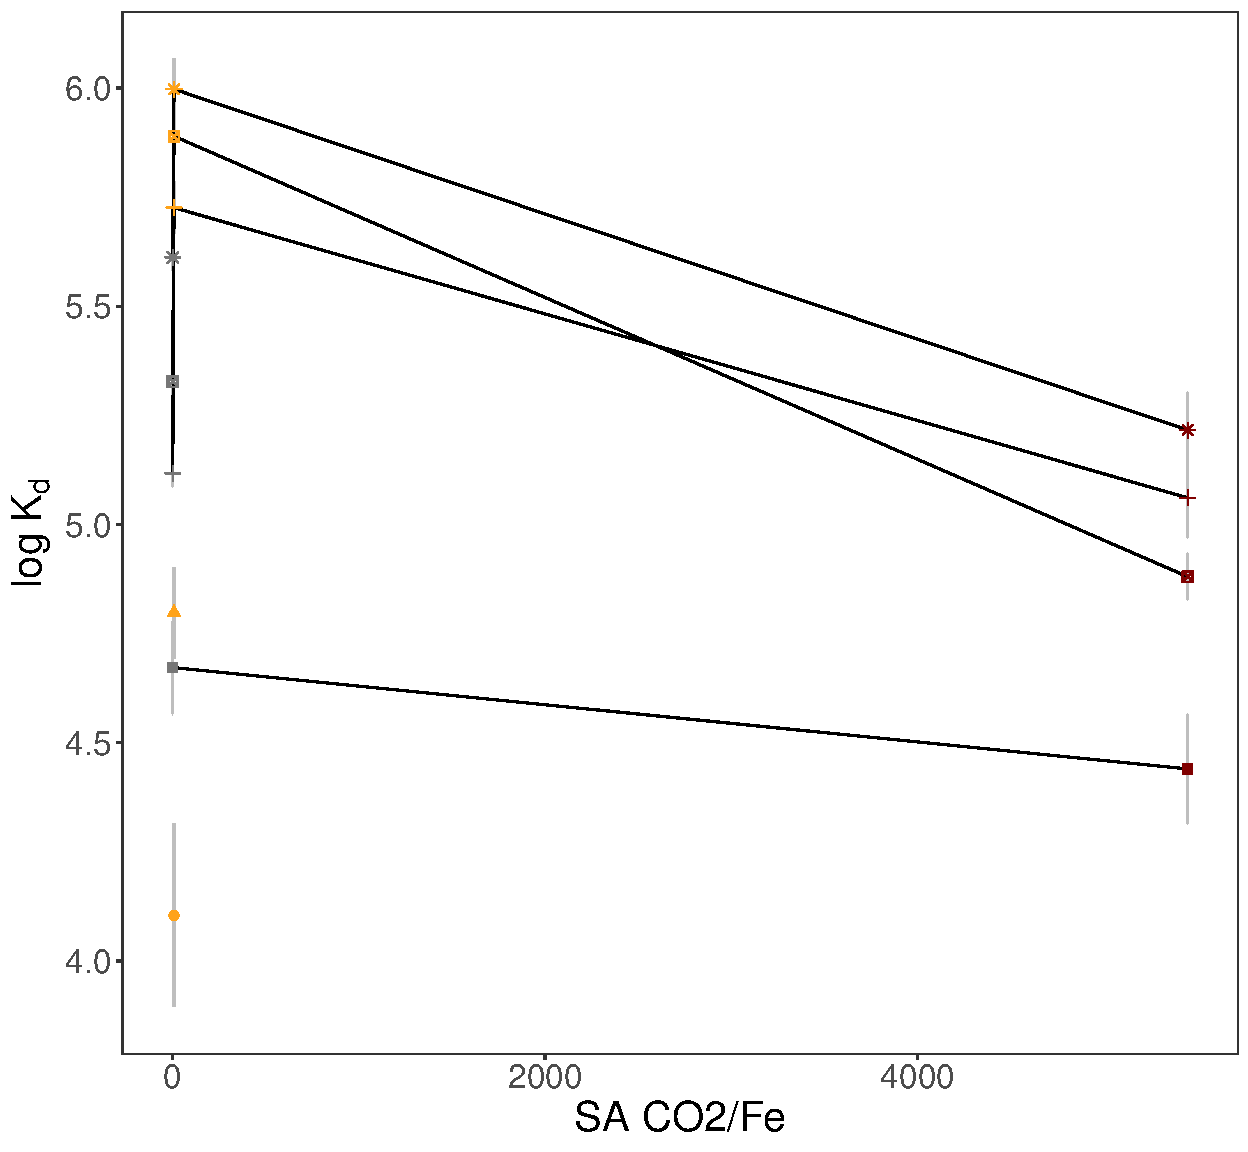
\includegraphics[height=5cm]{R/figs/Kd_1ugL_SACO2_Fe.pdf}
        \caption{}
        \label{subfig:SACO2_Fe}
    \end{subfigure}
    \medskip
    \begin{subfigure}[t]{0.5\textwidth}
        \centering
        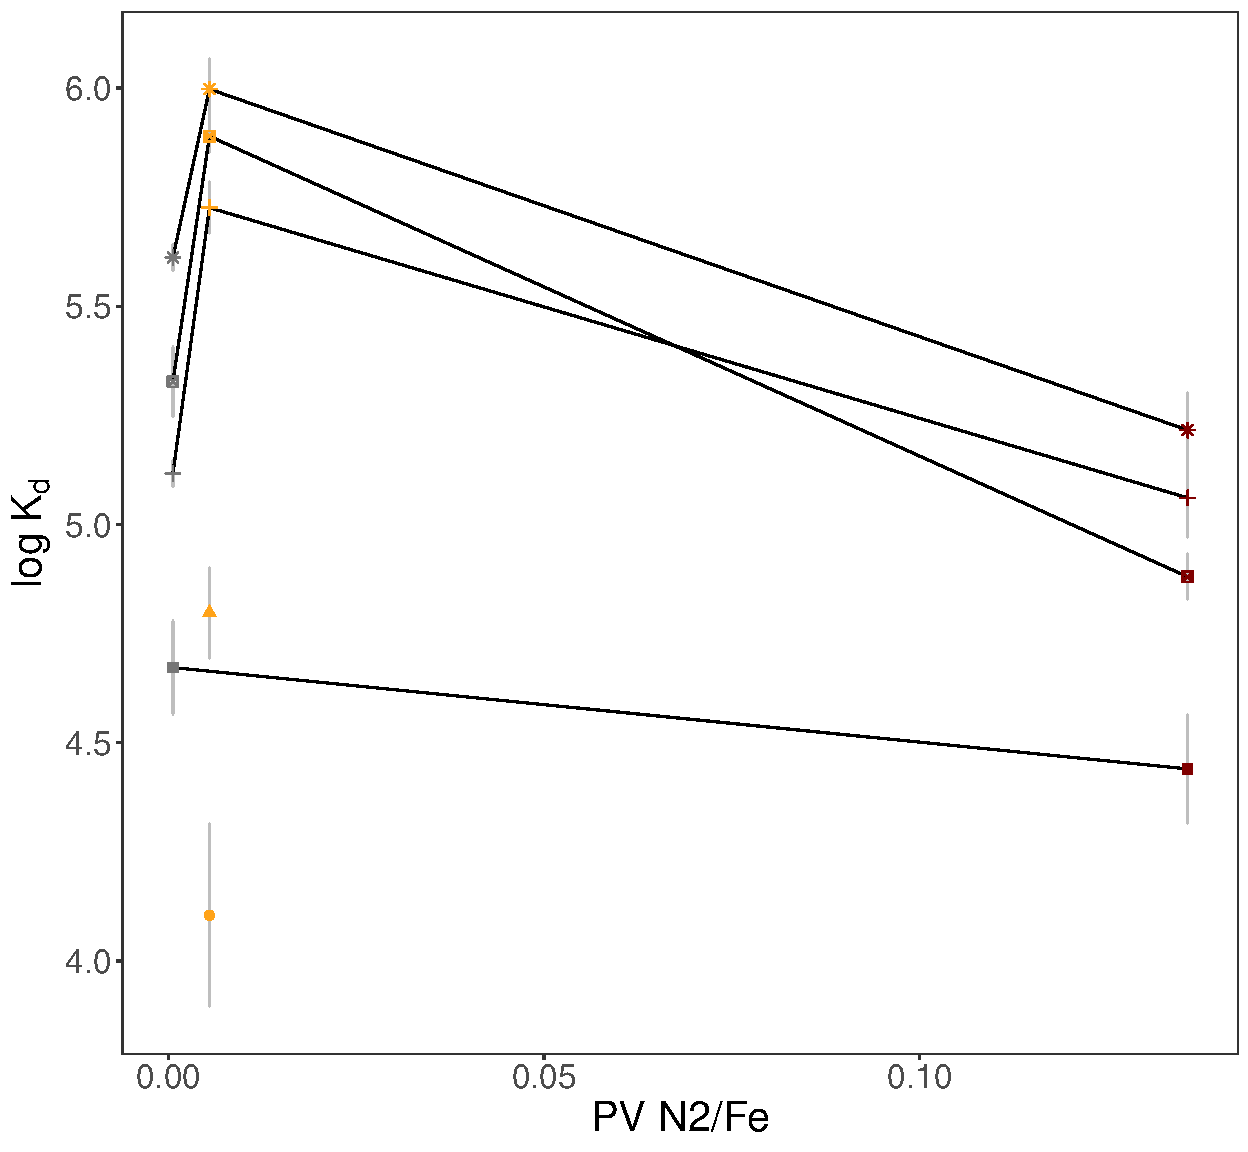
\includegraphics[height=5cm]{R/figs/Kd_1ugL_PVN2_Fe.pdf}
        \caption{}
        \label{subfig:PVN2_Fe}
    \end{subfigure}%
    ~ 
    \begin{subfigure}[t]{0.5\textwidth}
        \centering
        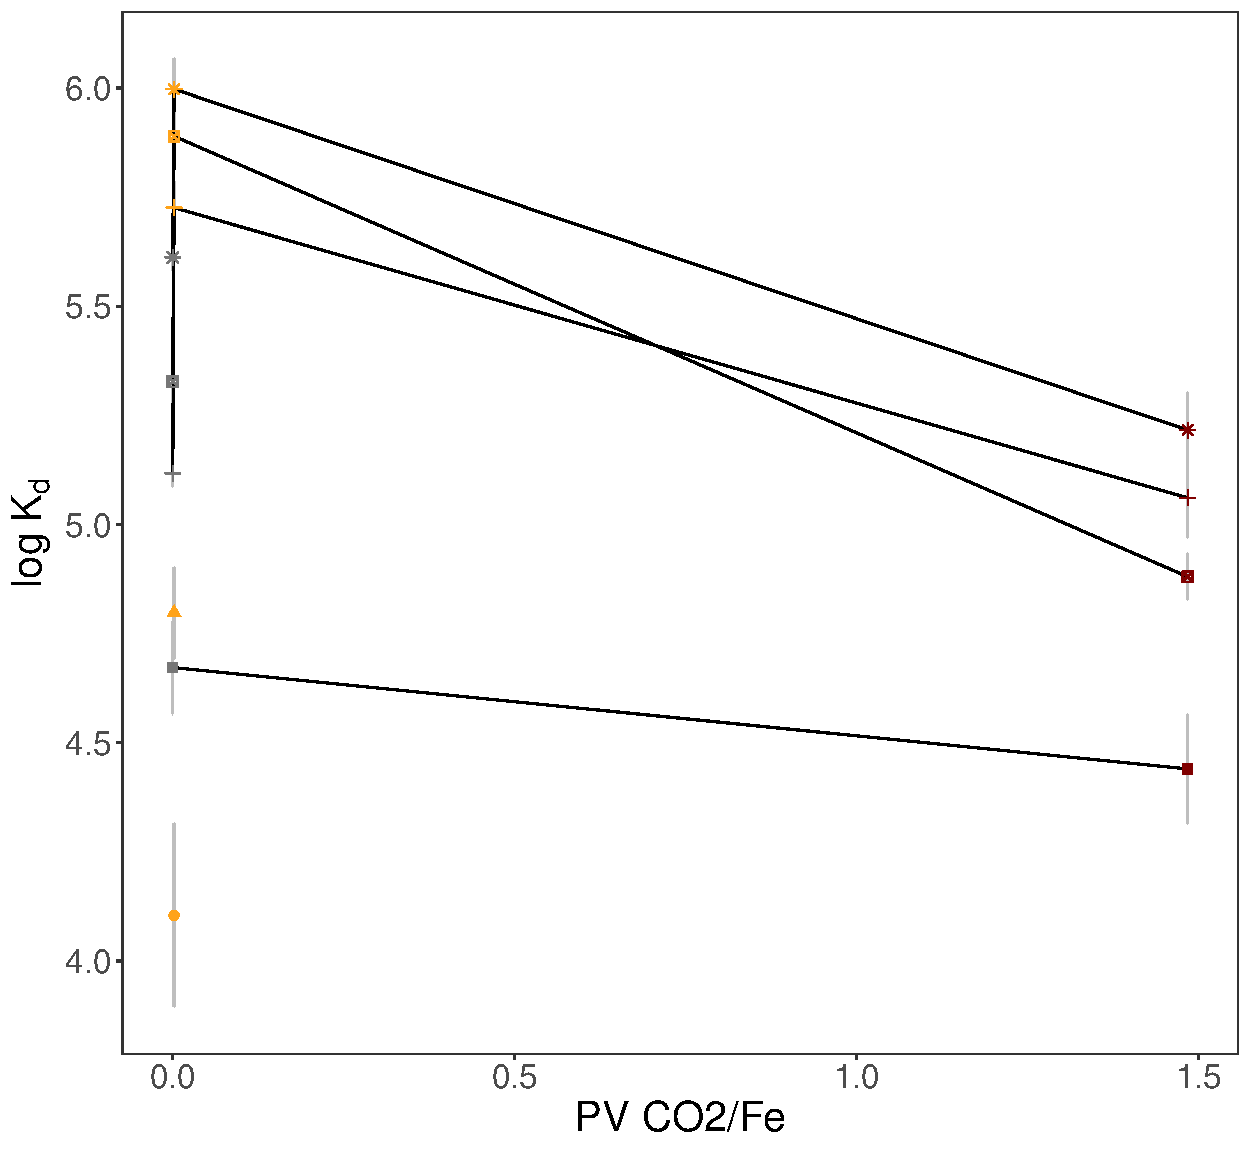
\includegraphics[height=5cm]{R/figs/Kd_1ugL_PVCO2_Fe.pdf}
        \caption{}
        \label{subfig:PVCO2_Fe}
    \end{subfigure}
    \label{fig:PVSA_Fe}
    \caption{}
\end{figure*}

\begin{figure}[!ht]
\subfloat[\label{subfig:SA_large}]{%
  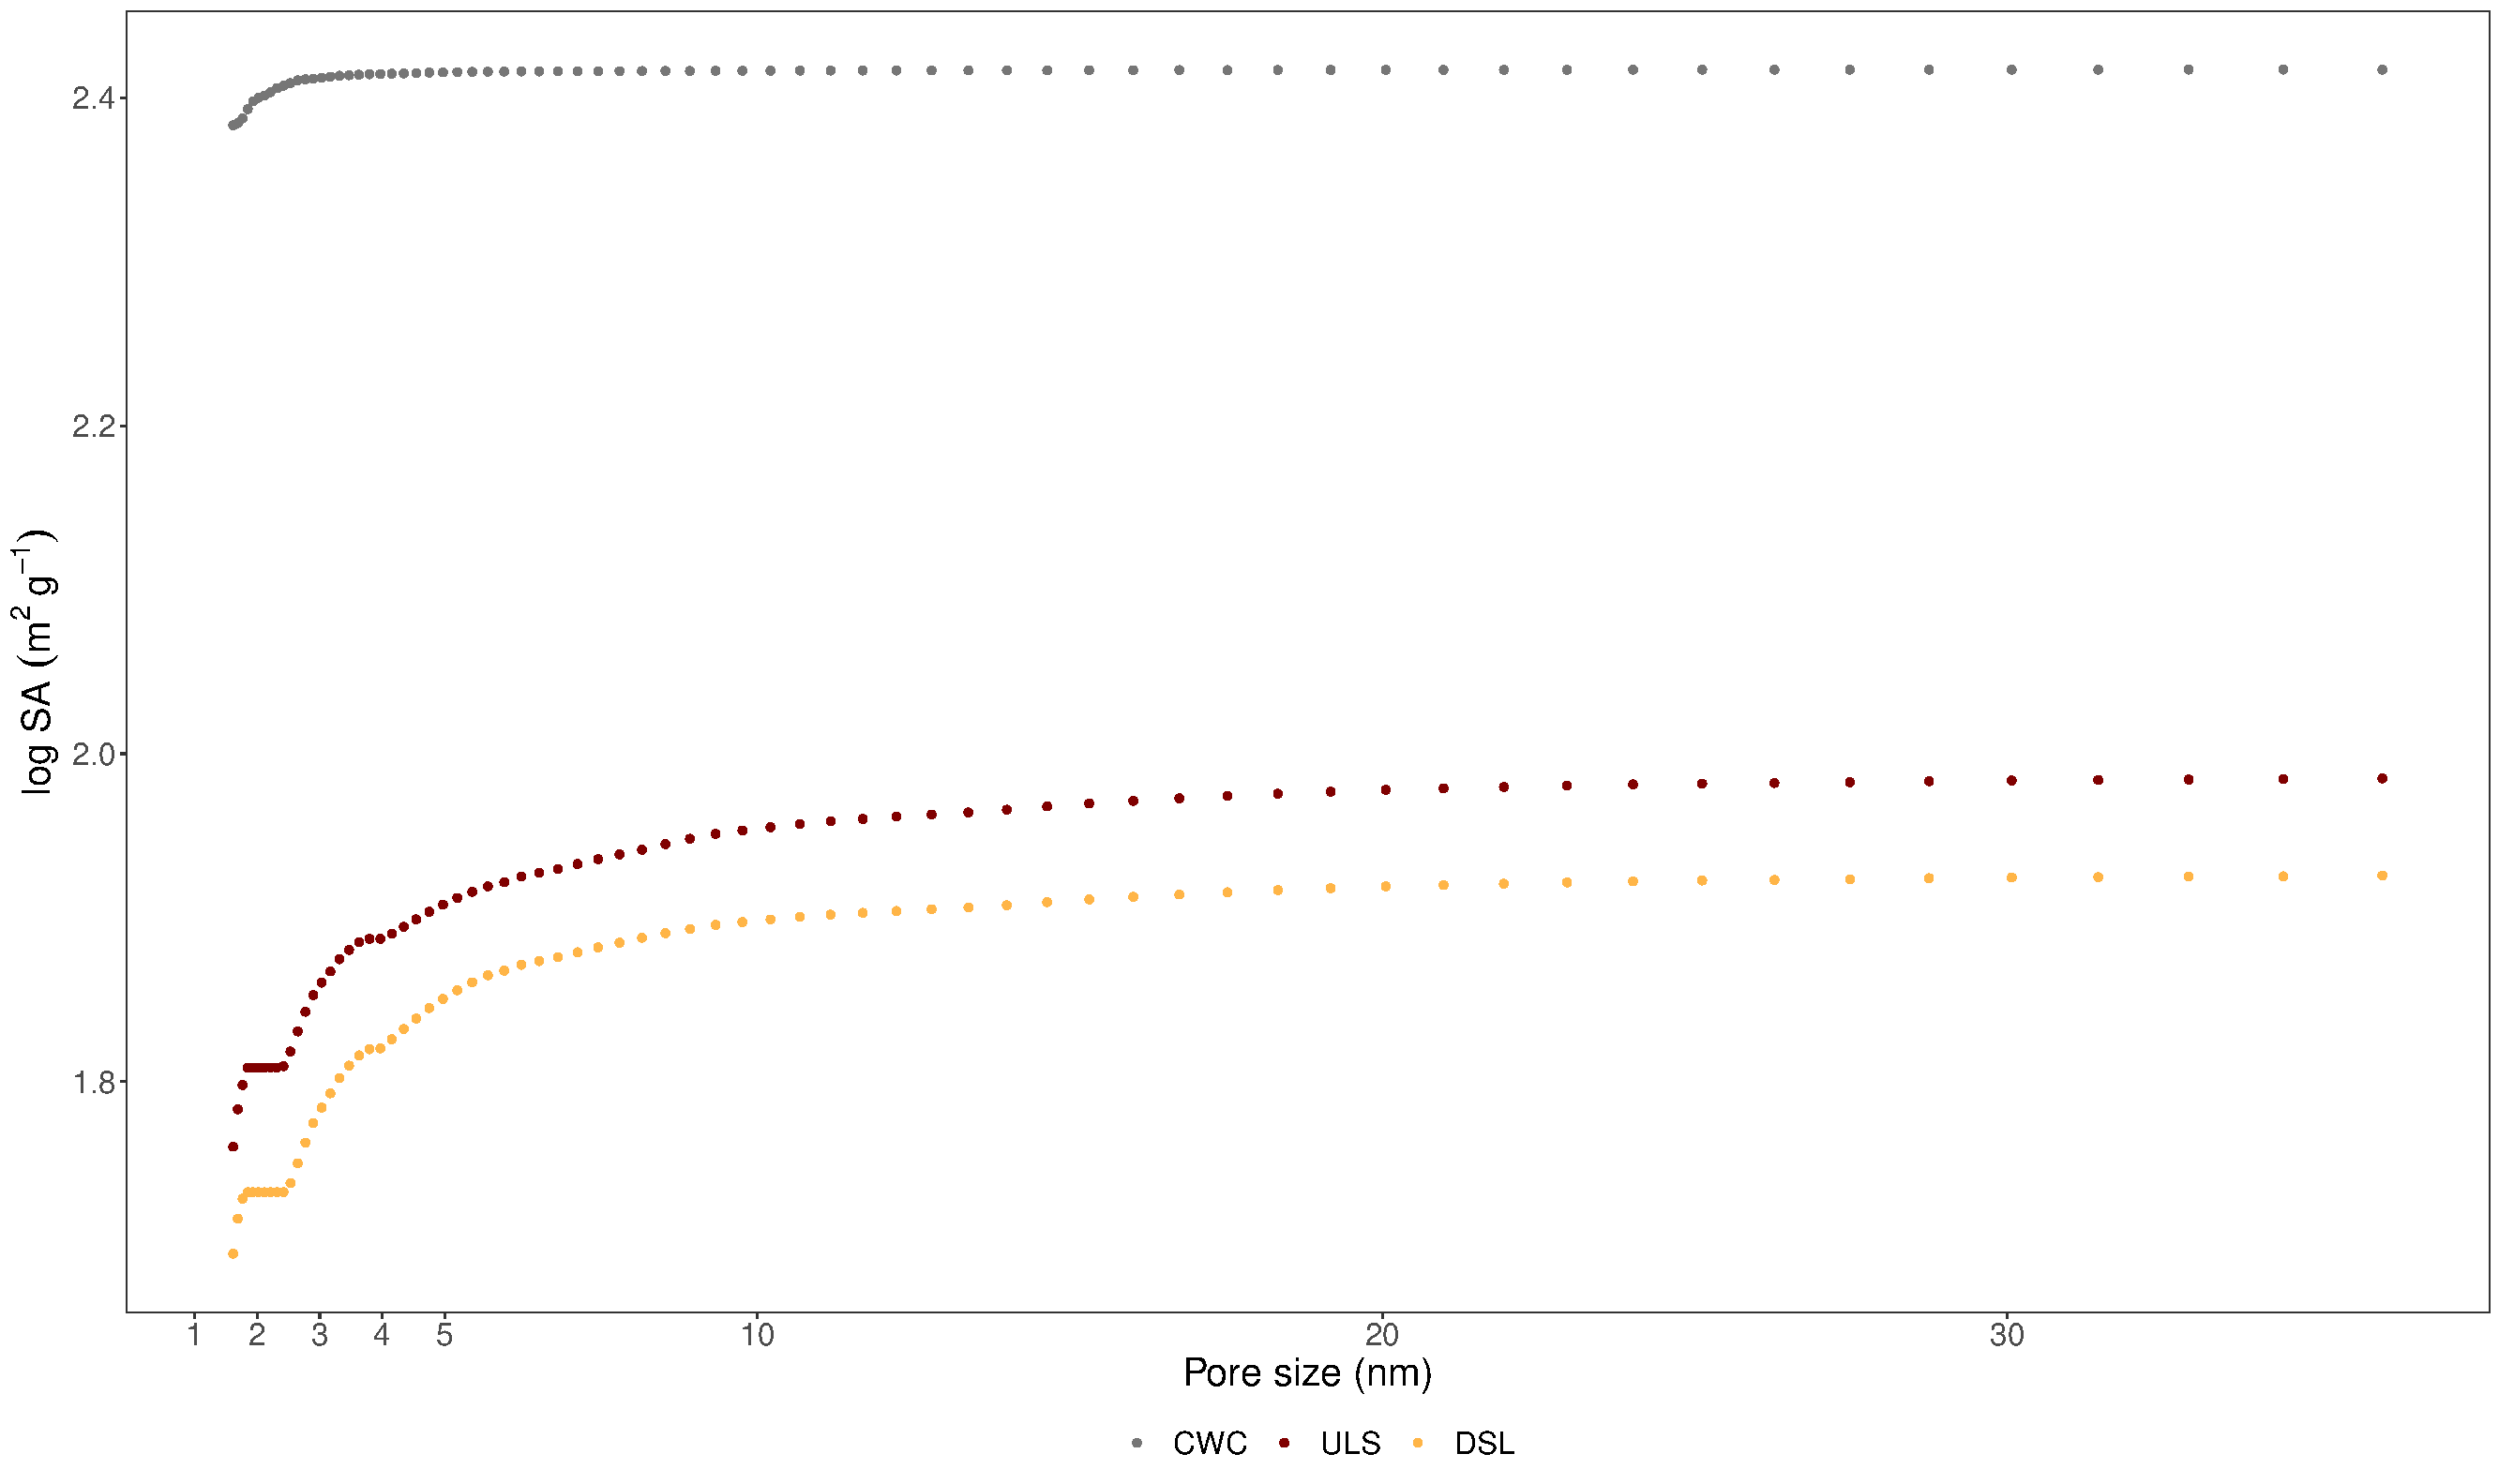
\includegraphics[width=0.5\textwidth]{R/figs/SA_large.pdf}
}
\hfill
\subfloat[\label{subfig:PV_large}]{%
  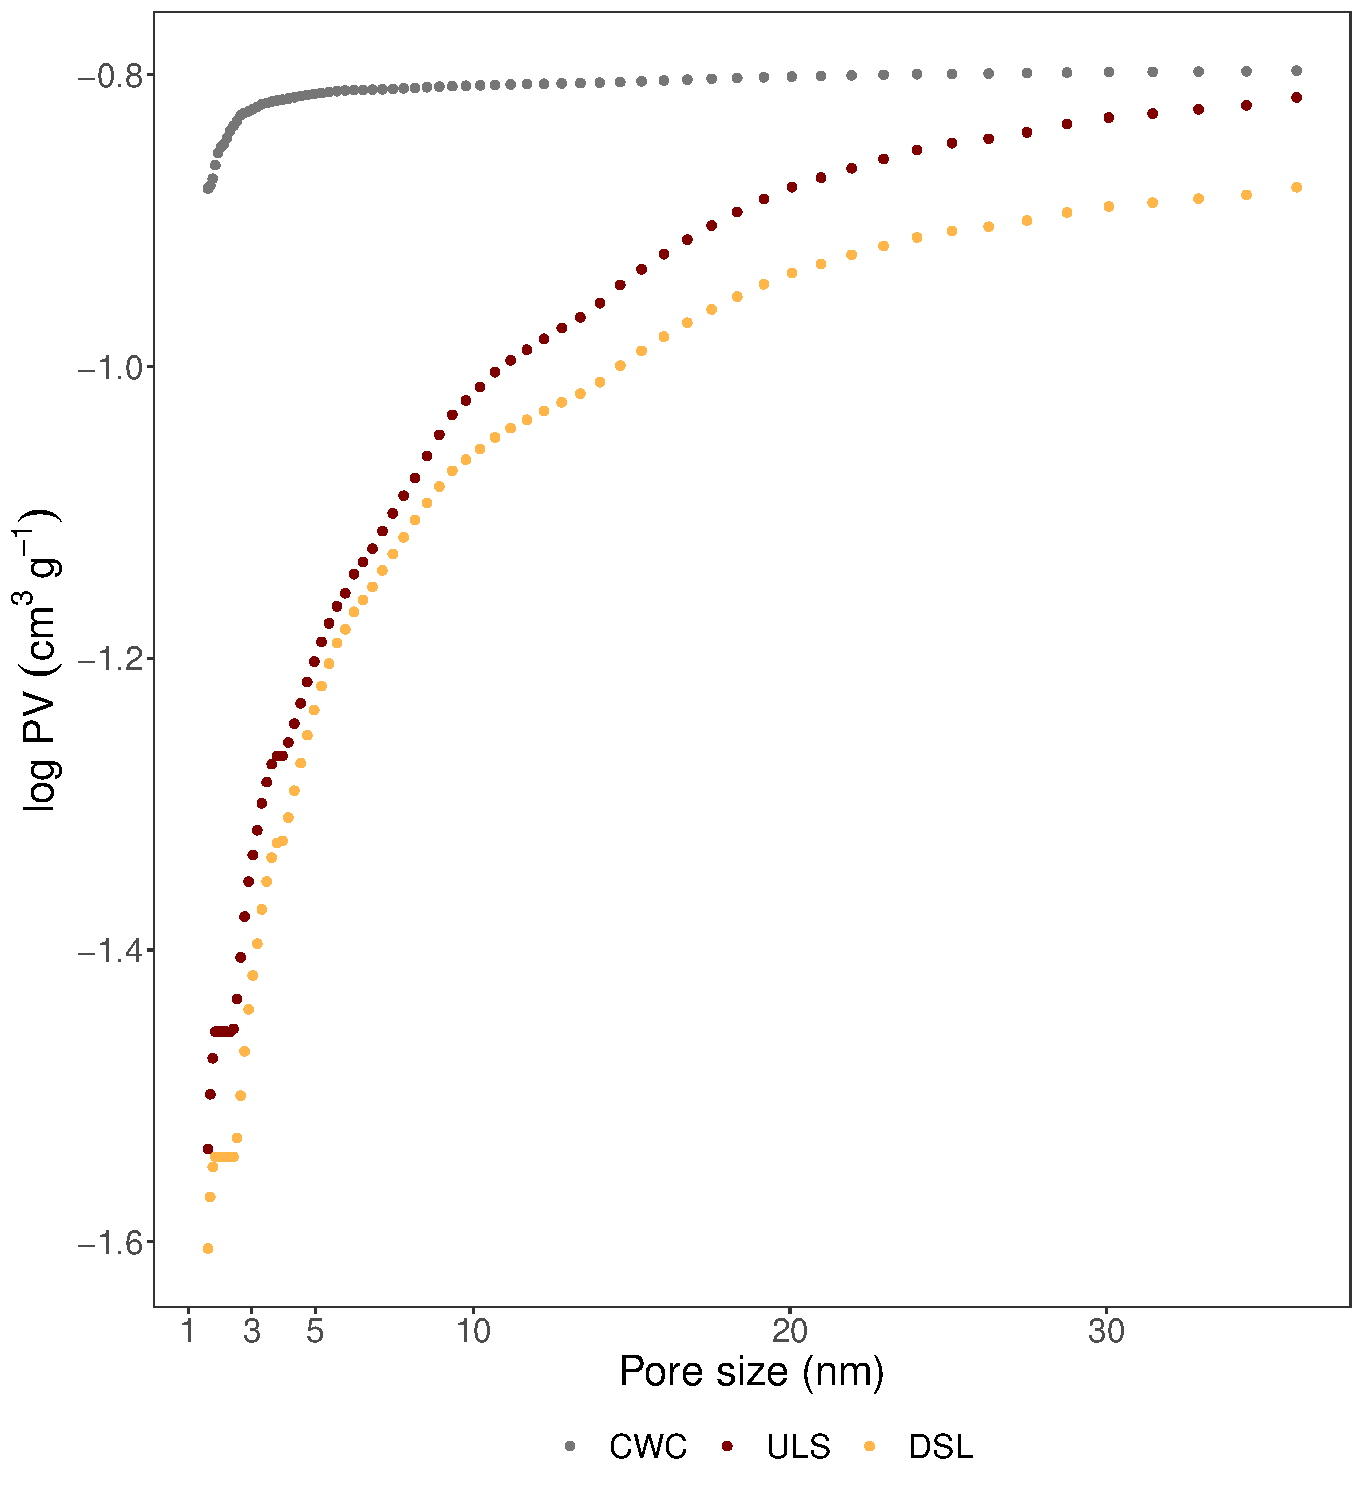
\includegraphics[width=0.5\textwidth]{R/figs/PV_large.pdf}
}
\medskip
\subfloat[\label{subfig:SAPV_large}]{%
  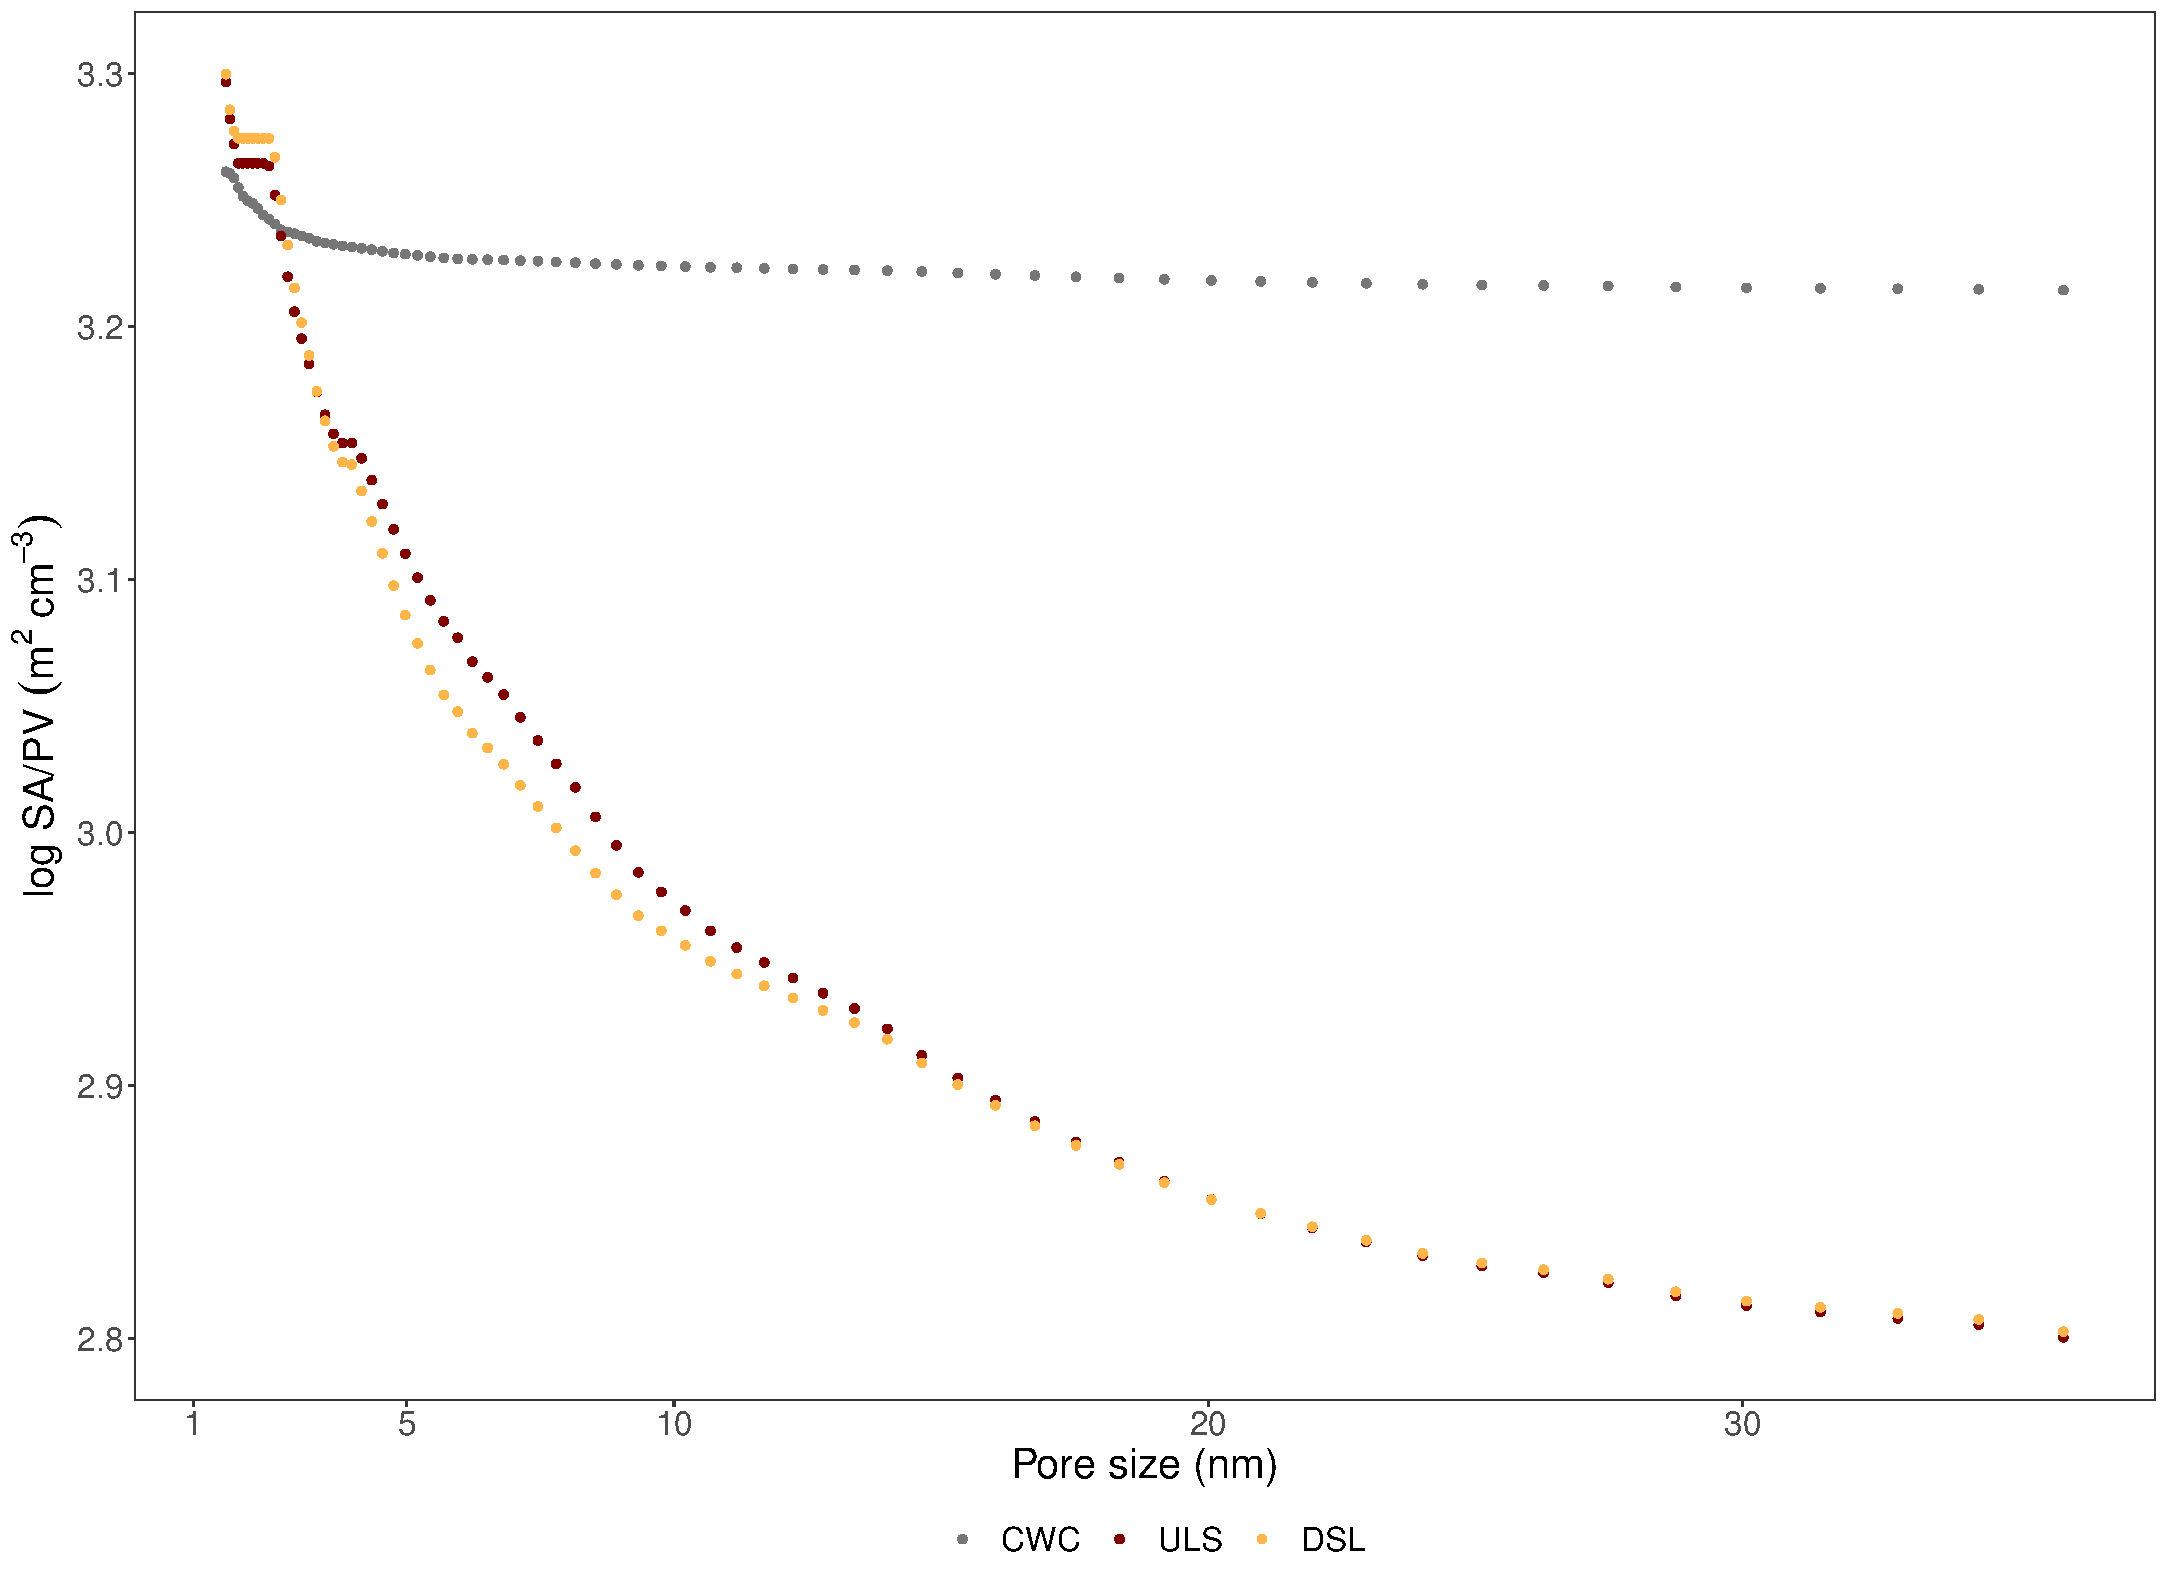
\includegraphics[width=0.5\textwidth]{R/figs/SAPV_large.pdf}
}
\hfill
\subfloat[\label{subfig:SAPV_C_large}]{%
  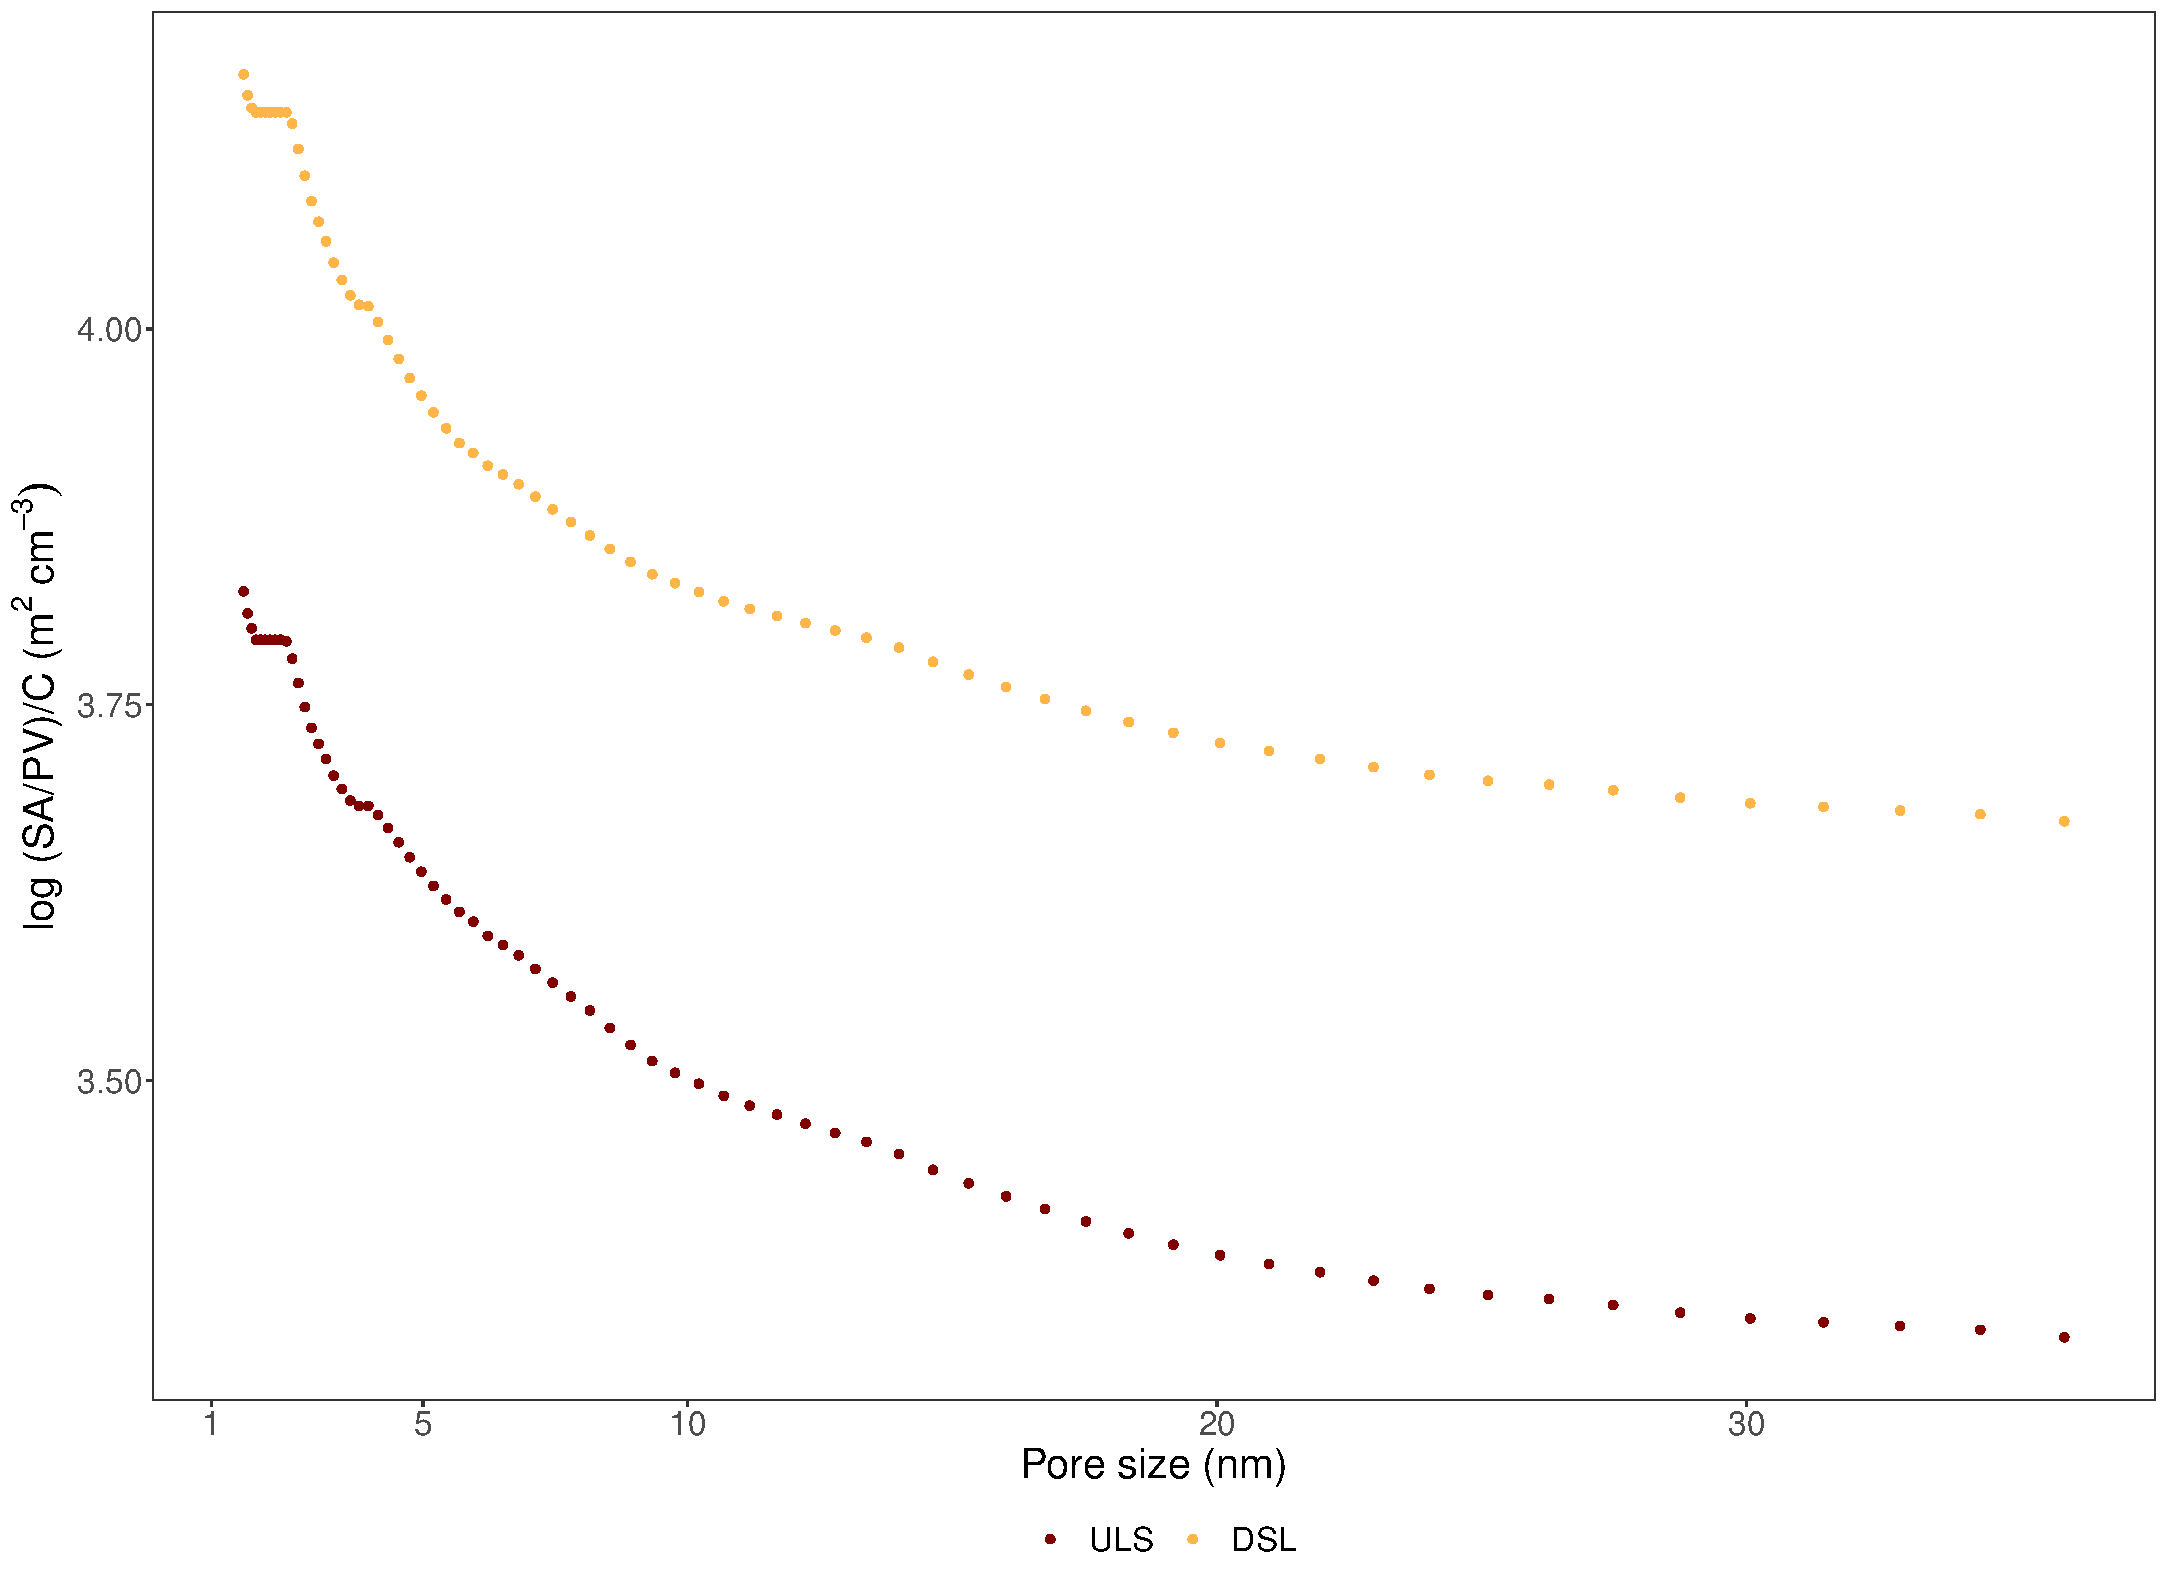
\includegraphics[width=0.5\textwidth]{R/figs/SAPV_C_large.pdf}
}
\caption{Pore size distribution for pores $>$ 1.5 nm. (a) Surface area, (b) pore volume, (c) SA/PV ratio for pores $>$1.5 nm normalized to carbon content (g C g BC\textsuperscript{-1}). (d) A lower SA/PV/C ratio indicates a higher degree of C in the pore wall matrix.}
\label{fig:PZD}
\end{figure}

\begin{figure*}[ht]
\centering
    \begin{subfigure}[t]{0.5\textwidth}
        \centering
        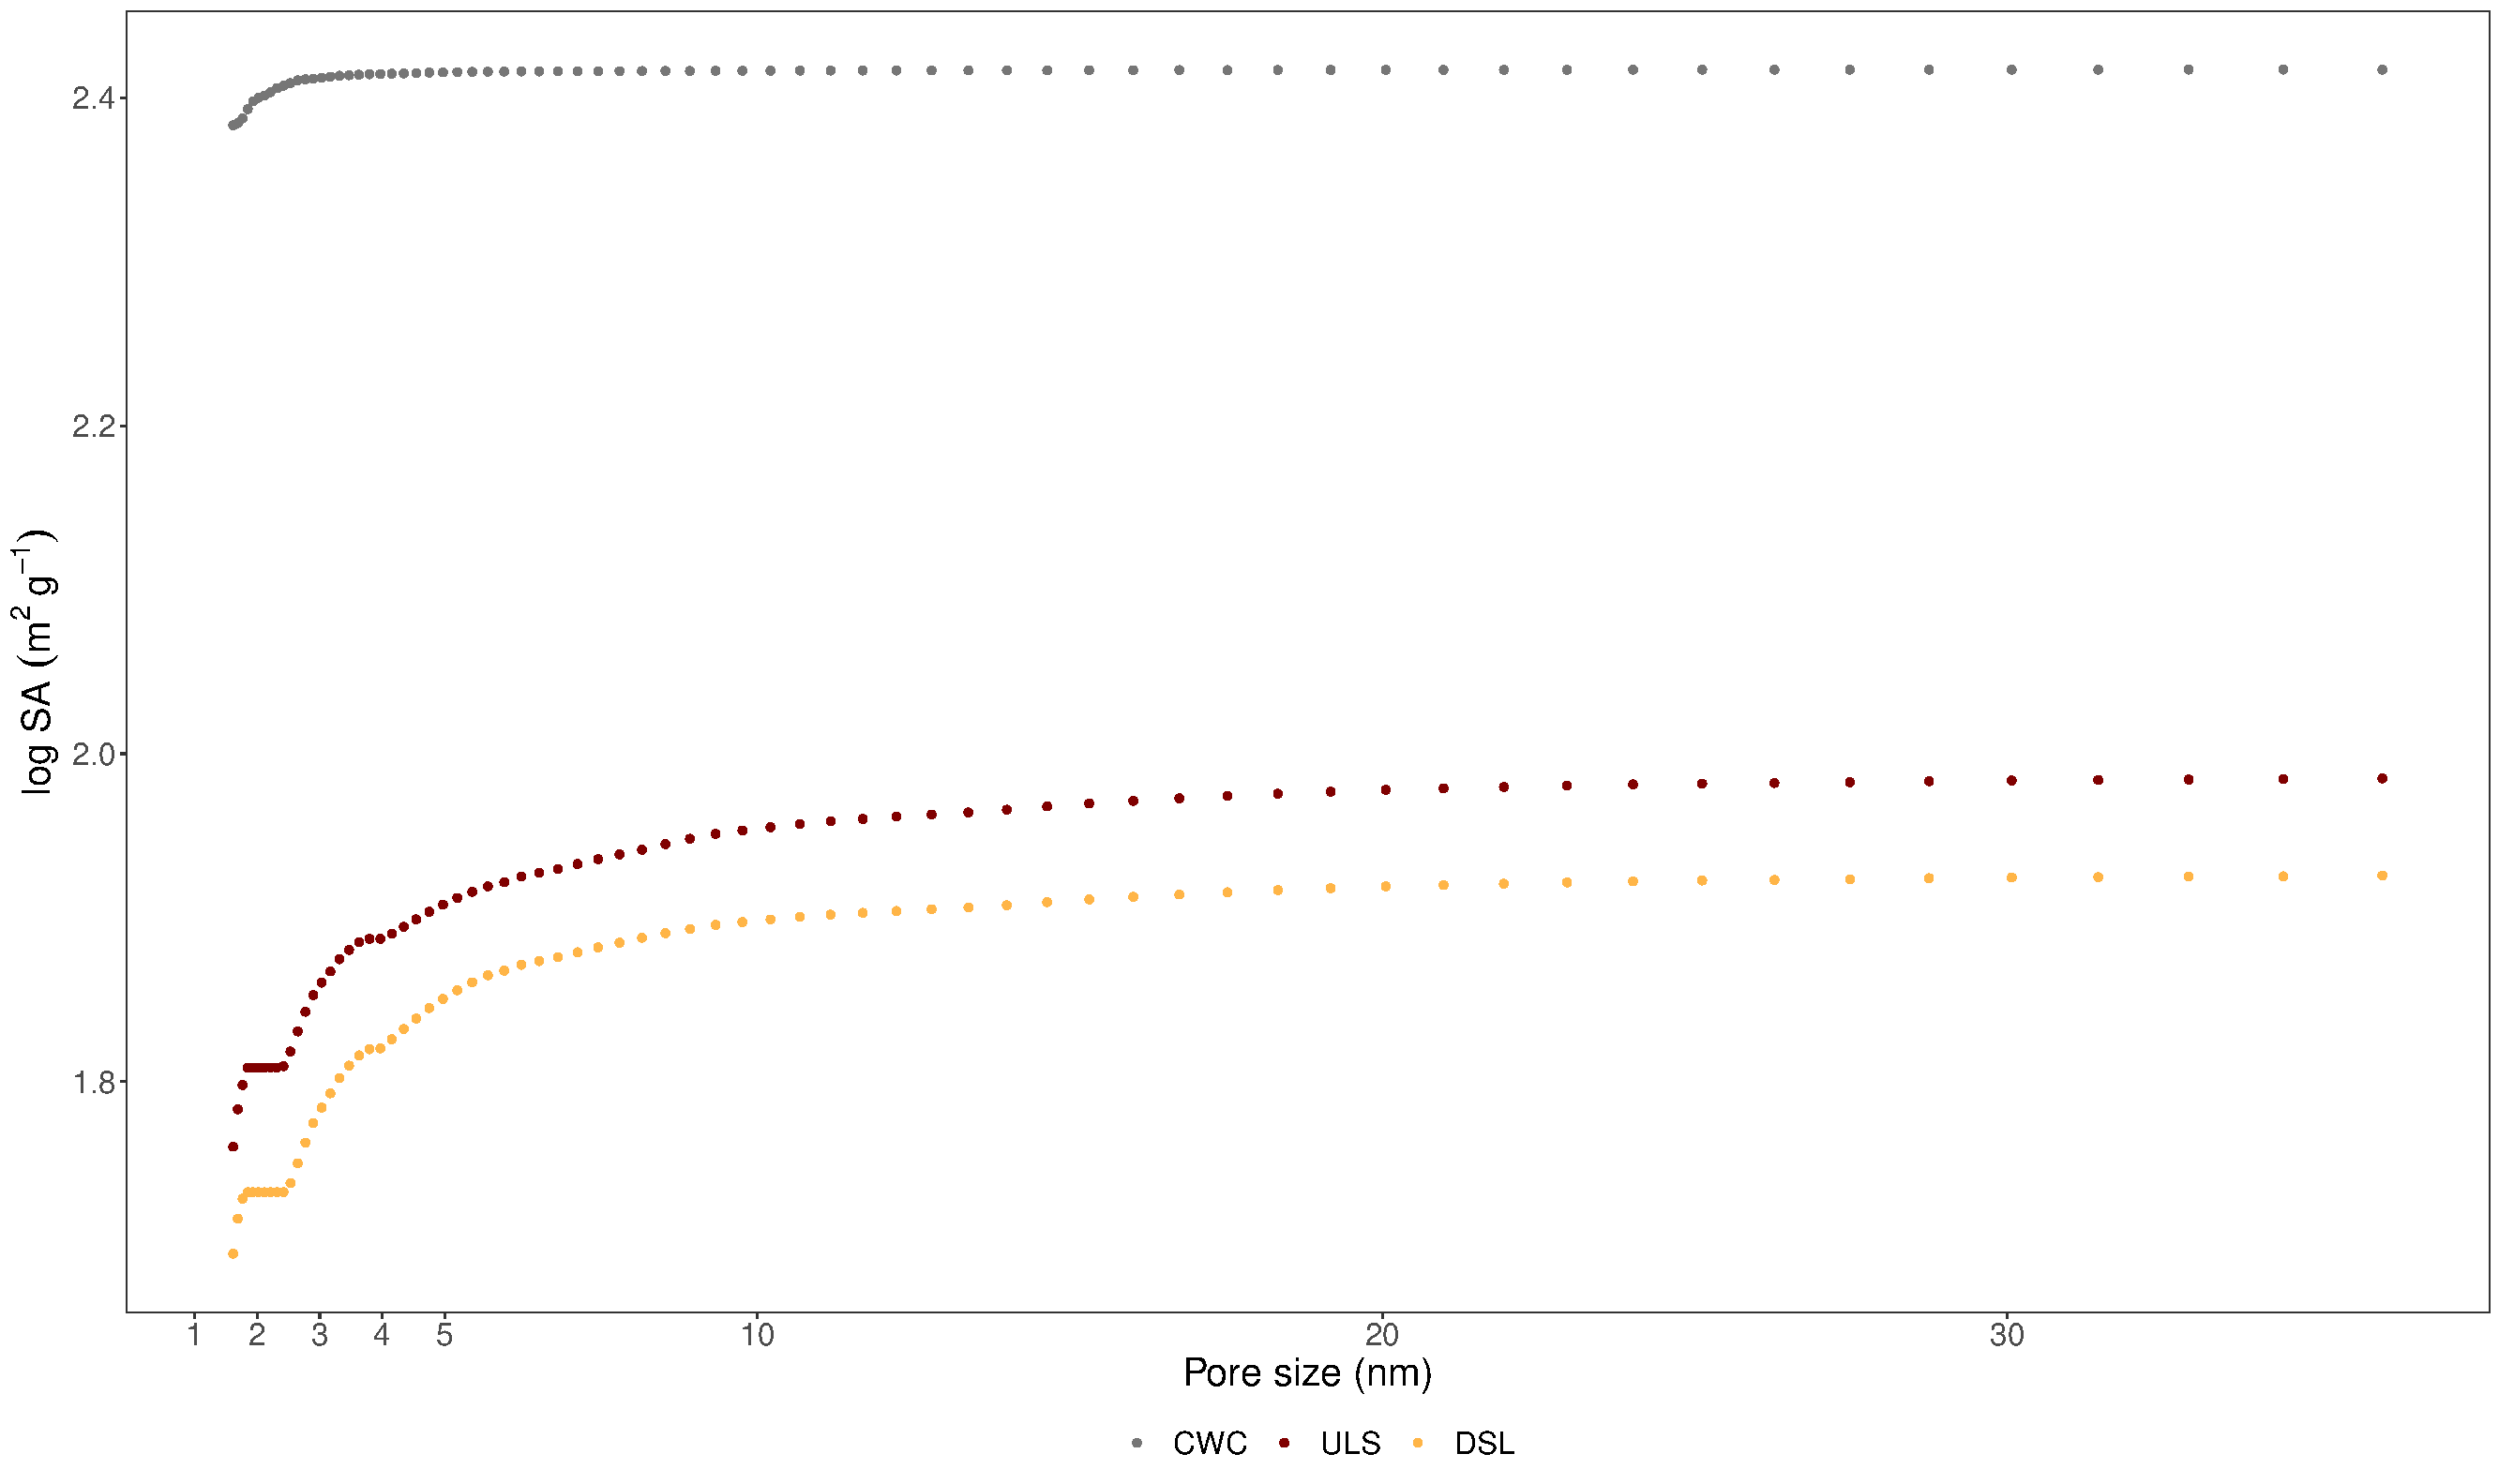
\includegraphics[\textwidth]{R/figs/SA_large.pdf}
        \caption{}
        \label{subfig:SA_large}
    \end{subfigure}%
    ~ 
    \begin{subfigure}[t]{0.5\textwidth}
        \centering
        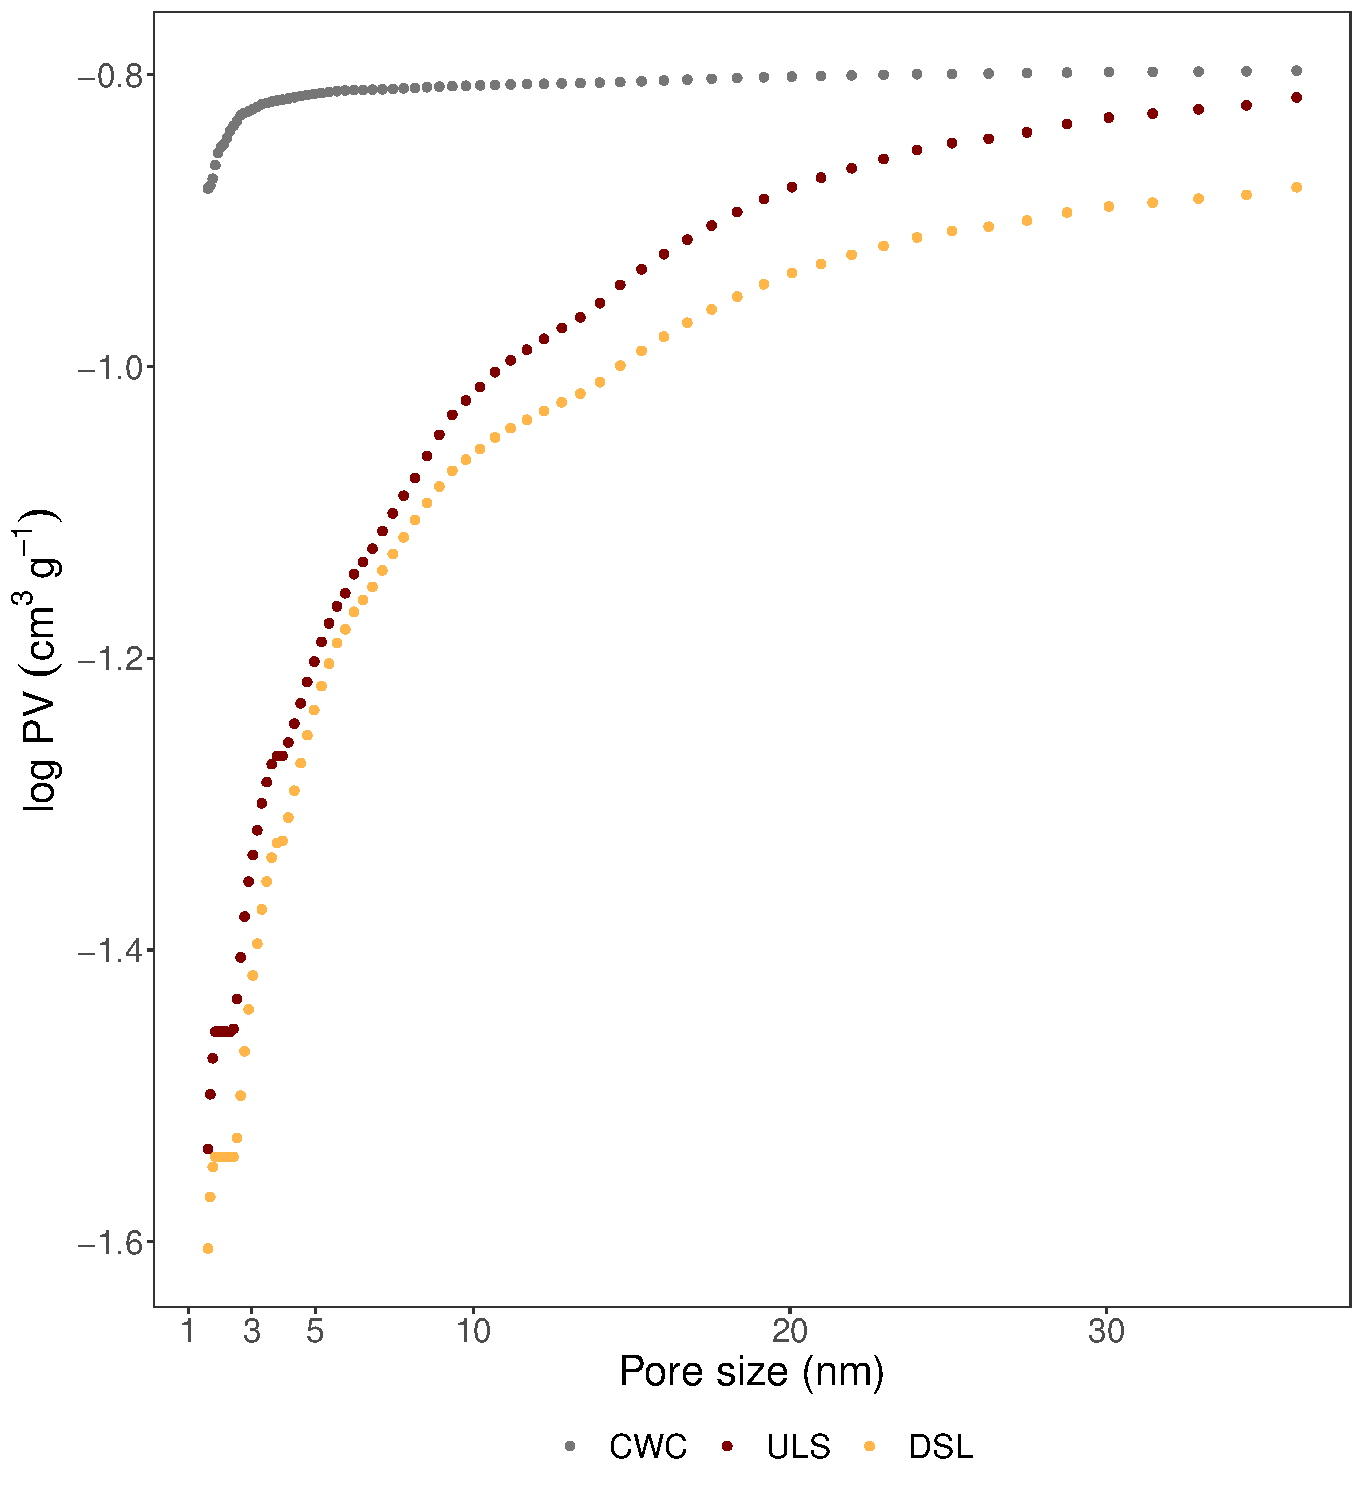
\includegraphics[\textwidth]{R/figs/PV_large.pdf}
        \caption{}
        \label{subfig:PV_large}
    \end{subfigure}
    \medskip
    \begin{subfigure}[t]{0.5\textwidth}
        \centering
        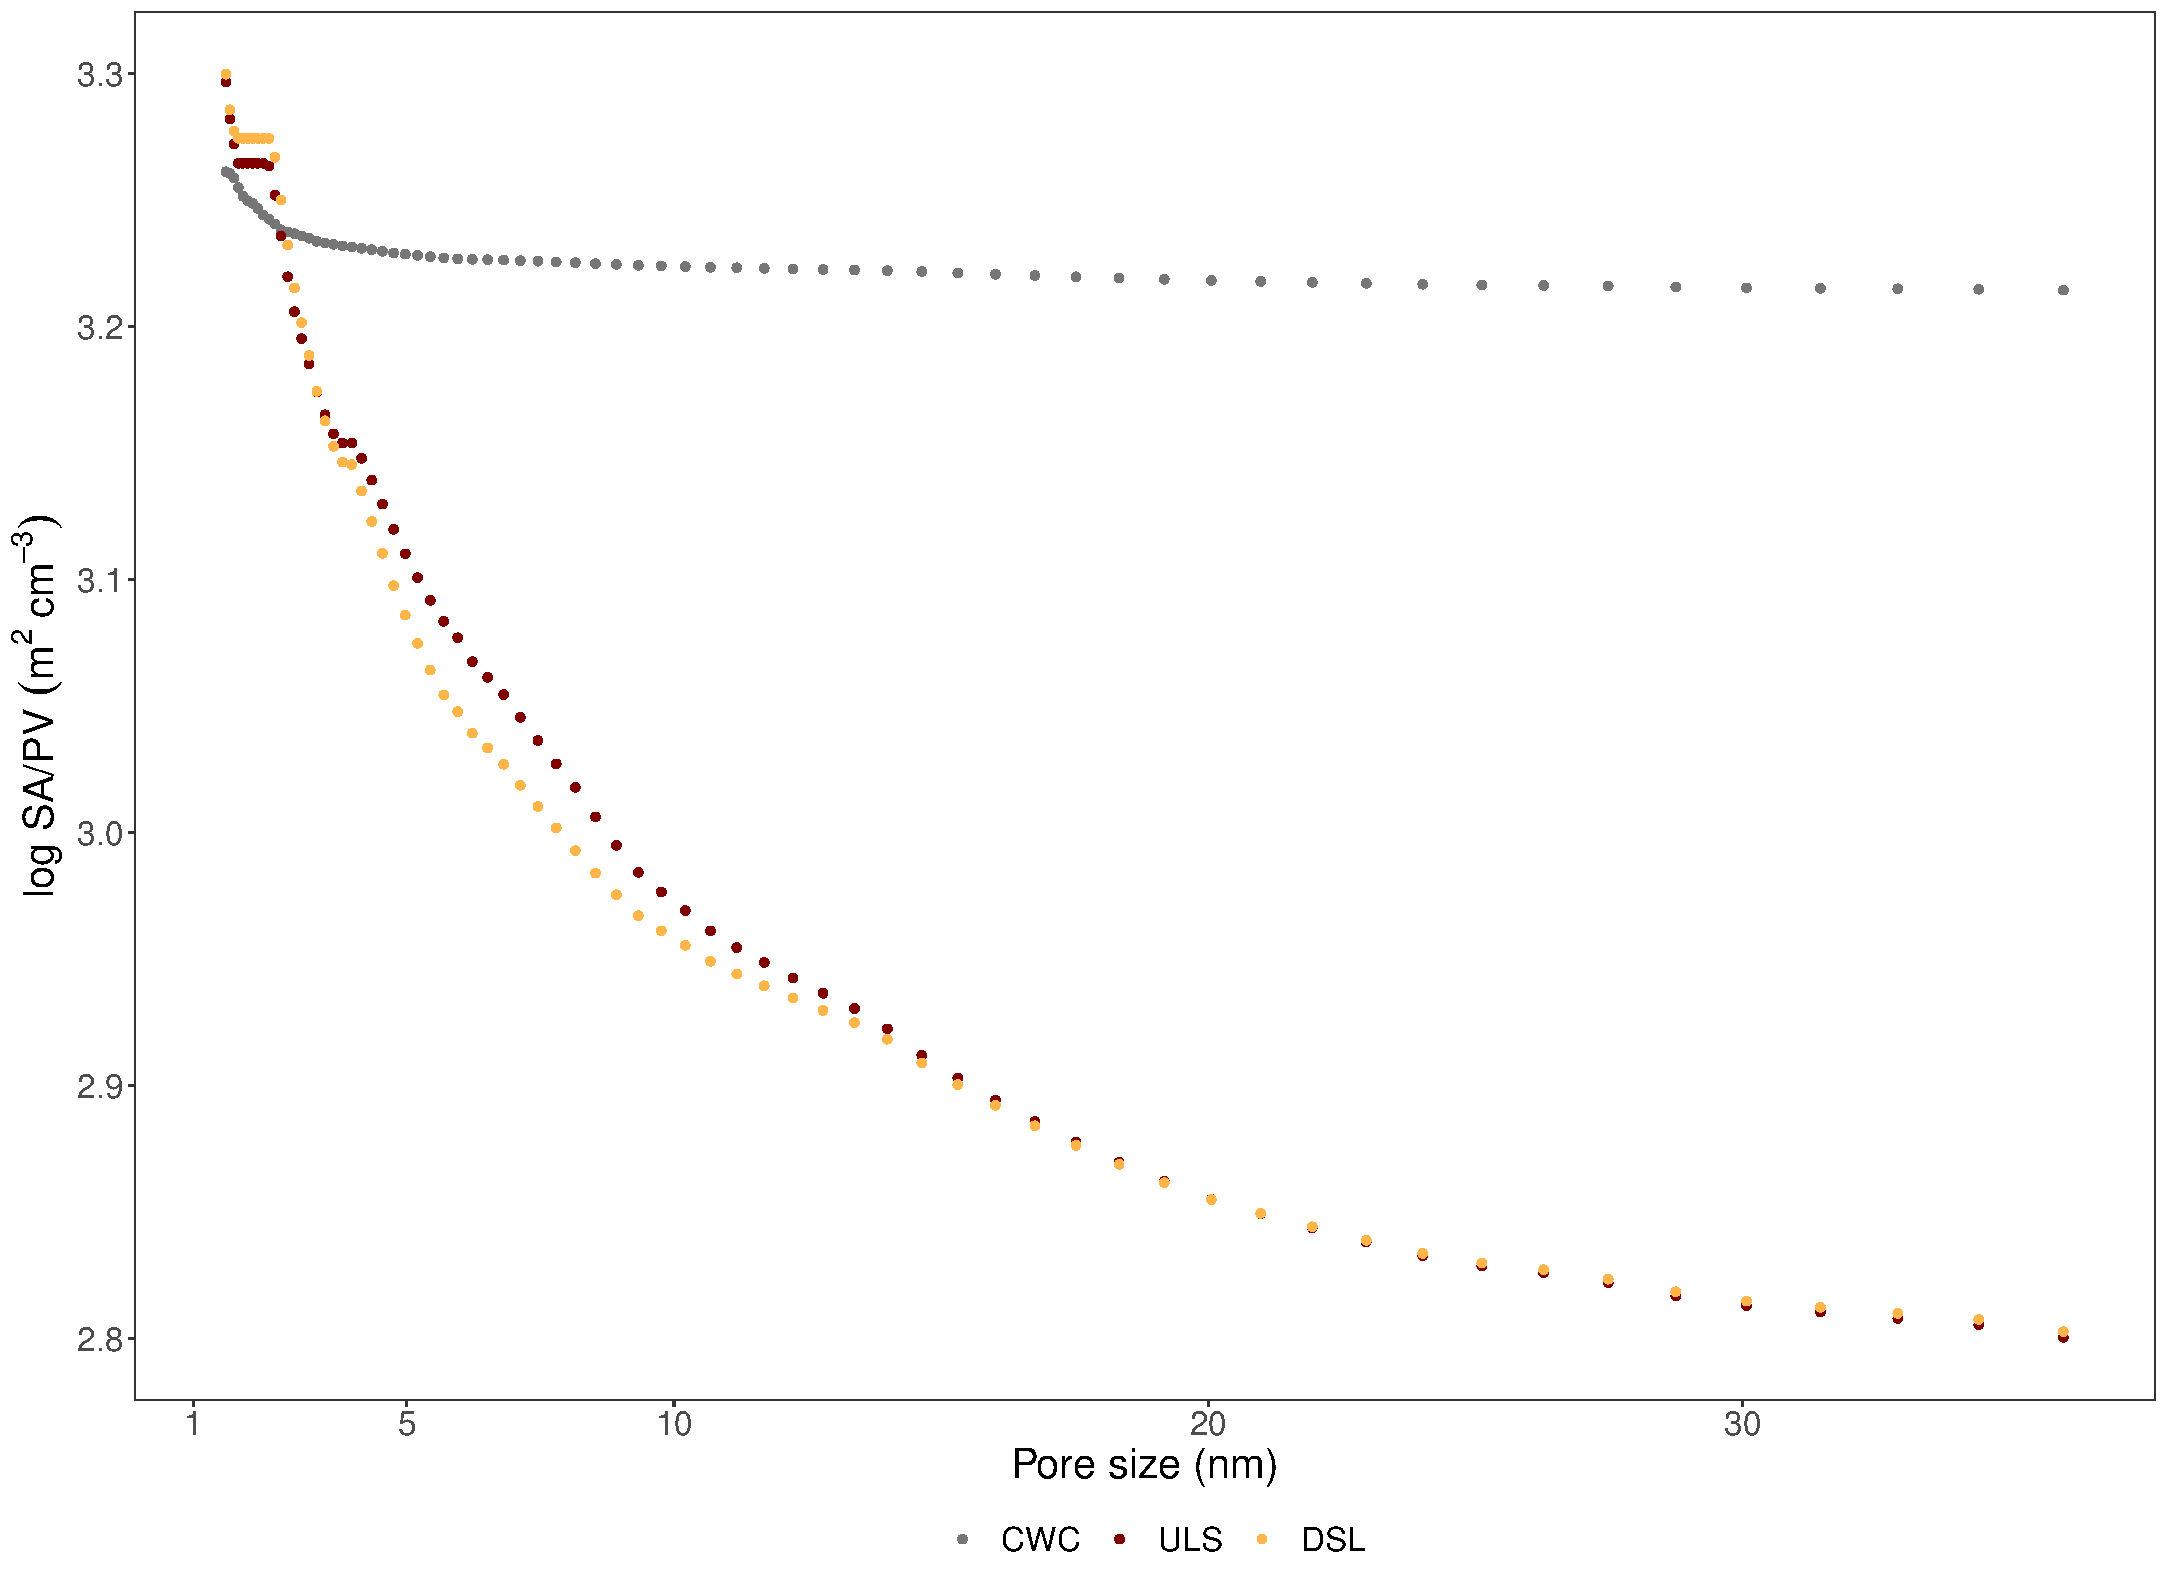
\includegraphics[\textwidth]{R/figs/SAPV_large.pdf}
        \caption{}
        \label{subfig:SAPV_large}
    \end{subfigure}%
    ~ 
    \begin{subfigure}[t]{0.5\textwidth}
        \centering
        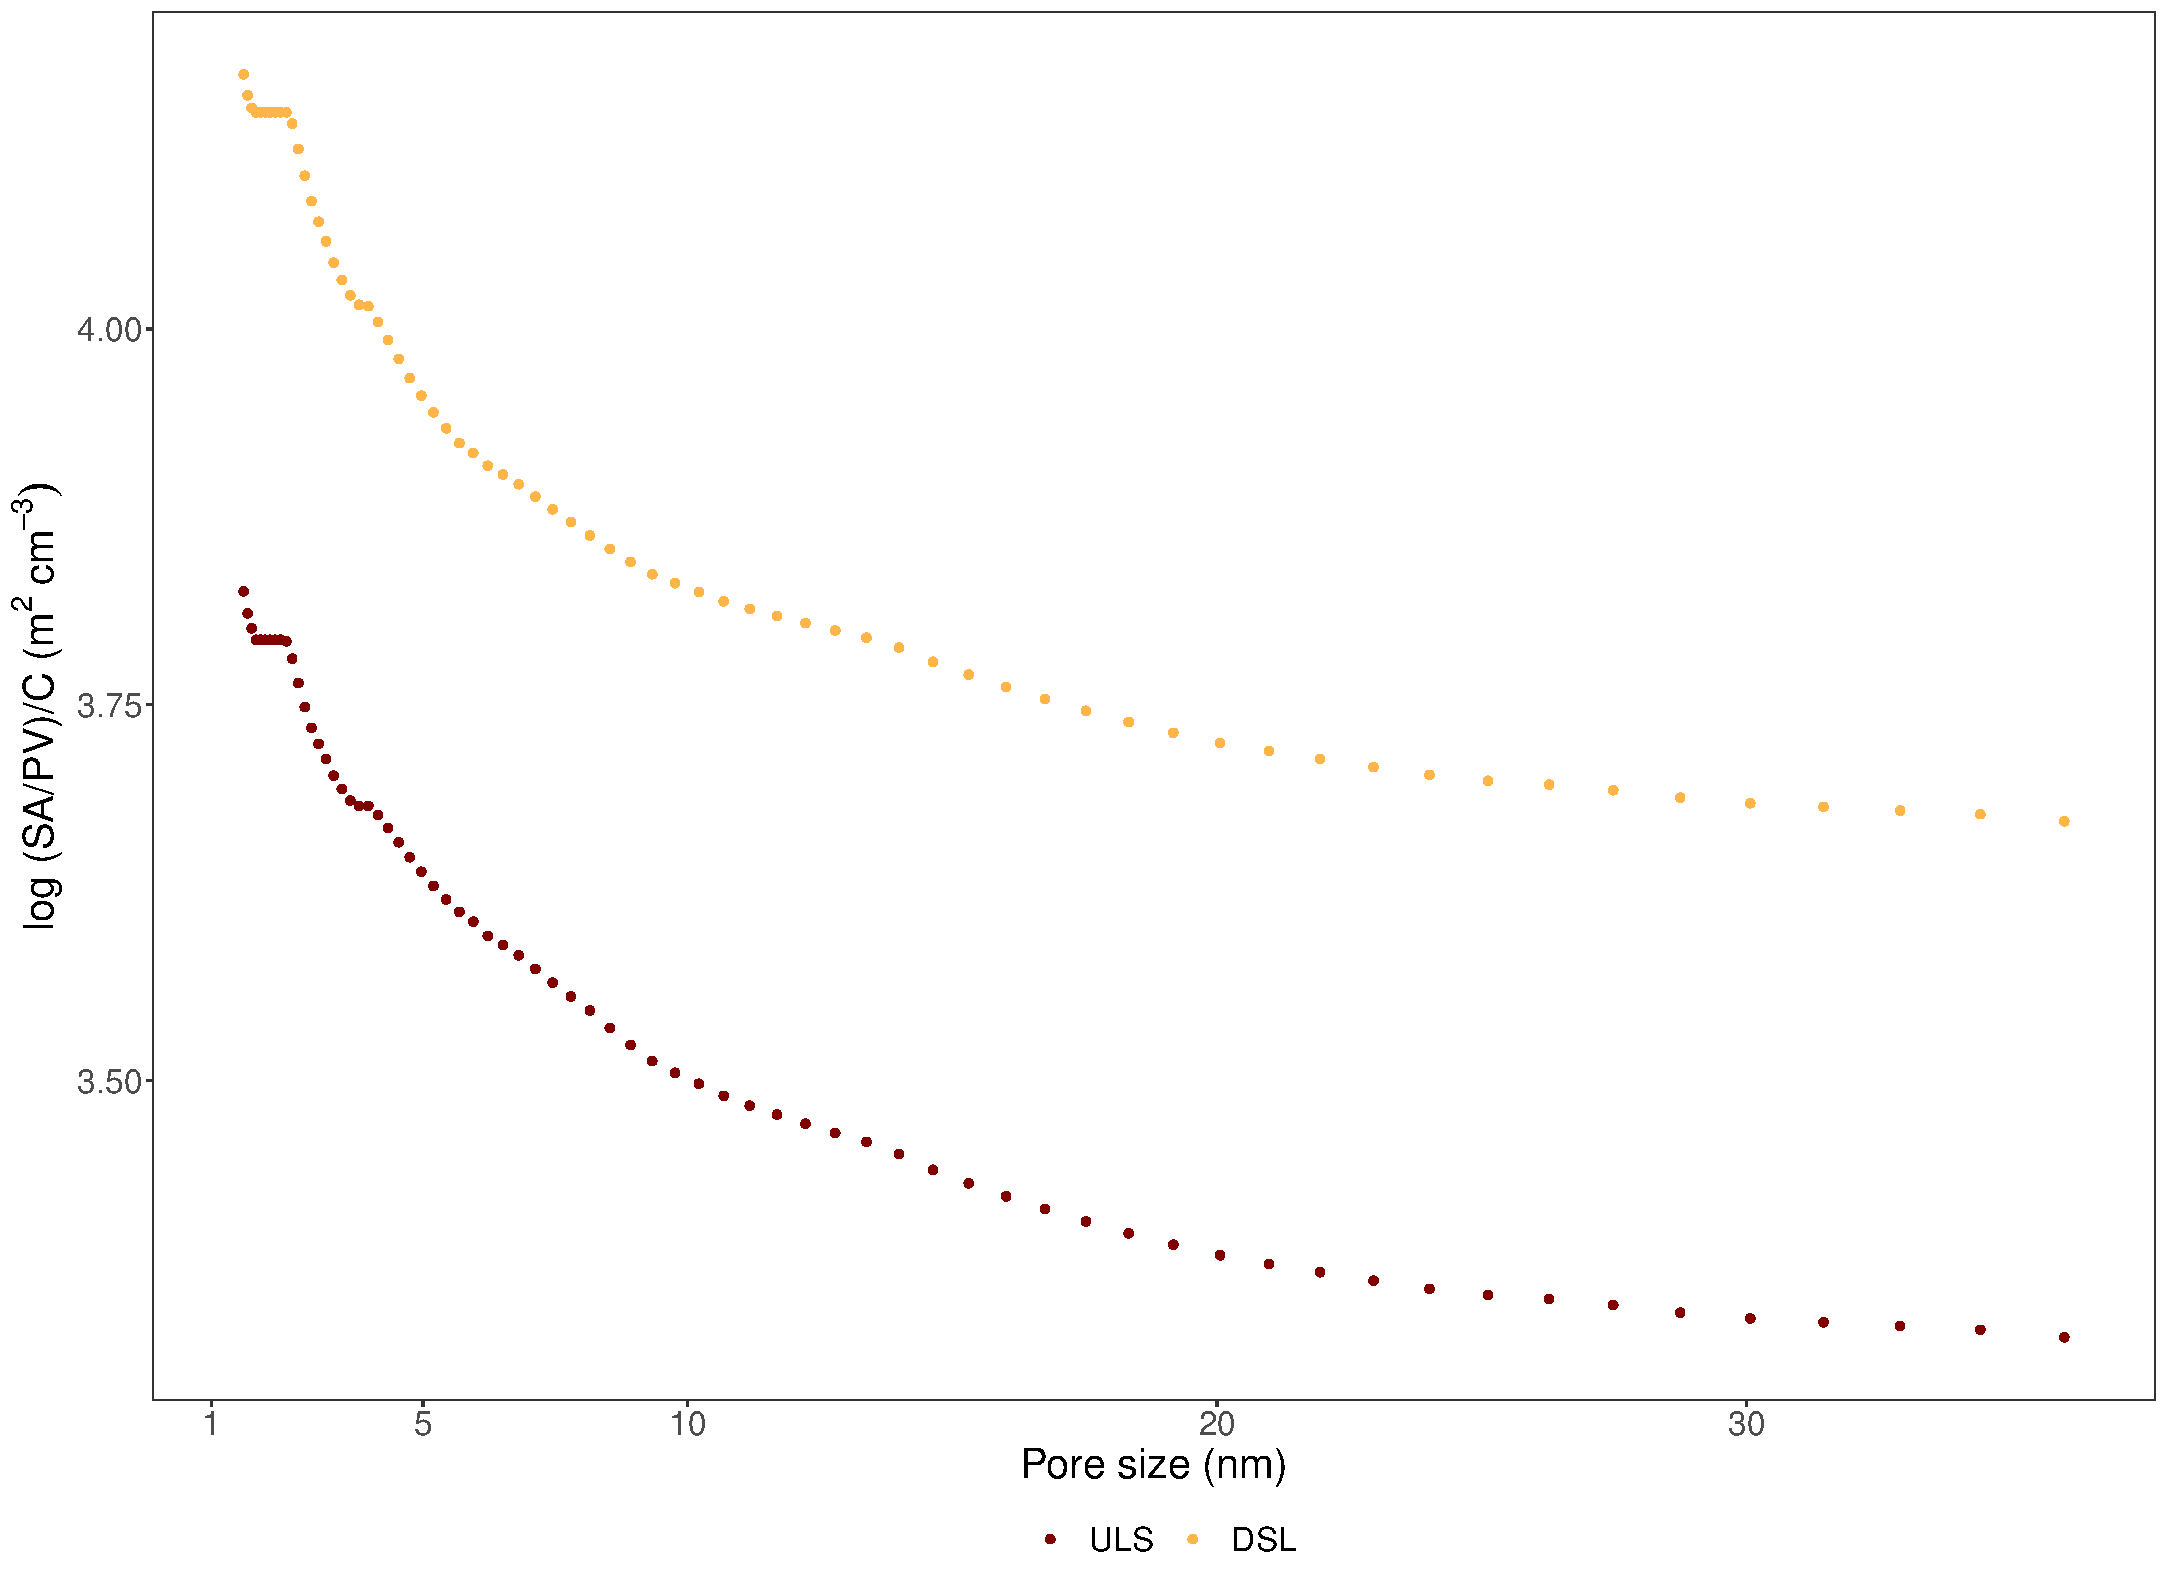
\includegraphics[\textwidth]{R/figs/SAPV_C_large.pdf}
        \caption{}
        \label{subfig:SAPV_C_large}
    \end{subfigure}
\caption{Pore size distribution for pores $>$ 1.5 nm. (a) Surface area, (b) pore volume, (c) SA/PV ratio for pores $>$1.5 nm normalized to carbon content (g C g BC\textsuperscript{-1}). (d) A lower SA/PV/C ratio indicates a higher degree of C in the pore wall matrix.}
\label{fig:PZD_large}
\end{figure*}

Pore size distribution is important for explaining sorption of PFAS of increasing chain lengths due to differences in molecular size. PFDA has a maximum diameter of 1.54 nm, and therefore experiences size exclusion for the smallest pores (0.5-1.5 nm) and can therefore only diffuse into the larger pores represented by N\textsubscript{2} (\textgreater 1.5 nm) (\cref{tab:molecsize}). Regardless of the critical separation at pore size greater/less than 1.5 nm, shorter-chain PFCAs is expected to diffuse more easily into the pores than the larger compounds.  

\begin{figure}[!ht]
\subfloat[\label{subfig:Kd_C}]{%
  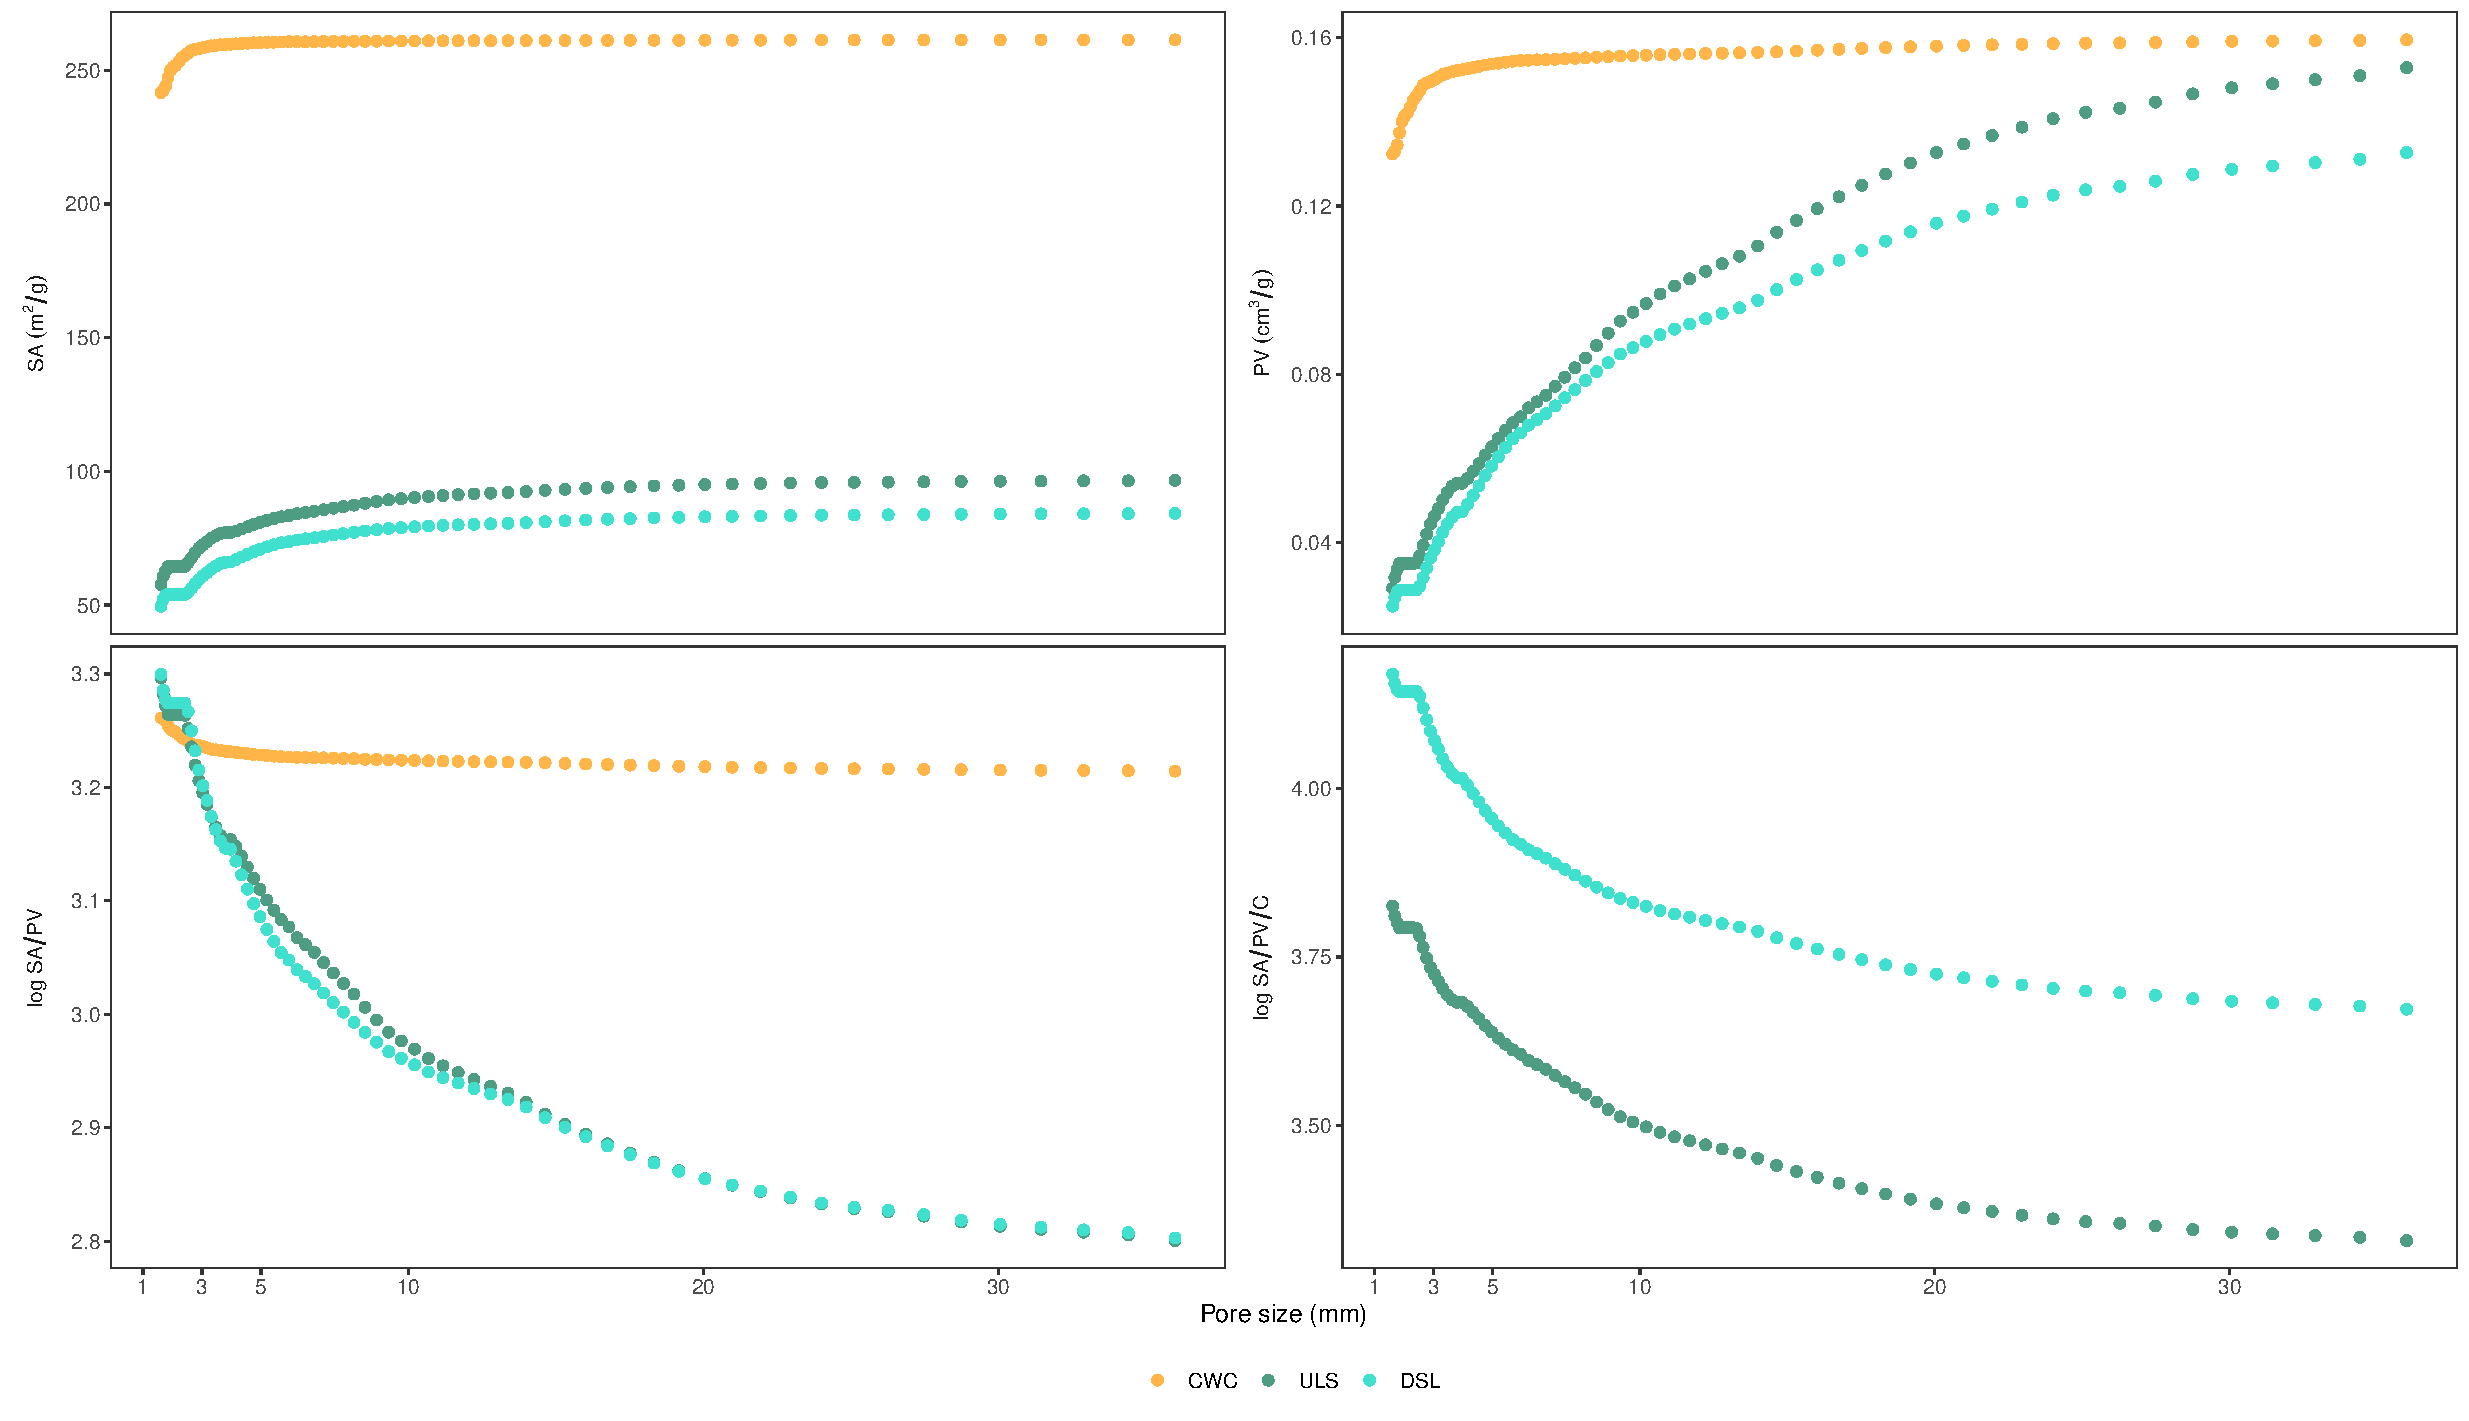
\includegraphics[width=0.3\textwidth]{R/figs/Kd_1ugL_C.pdf}
}
\hfill
\subfloat[\label{subfig:Kd_SAPV}]{%
  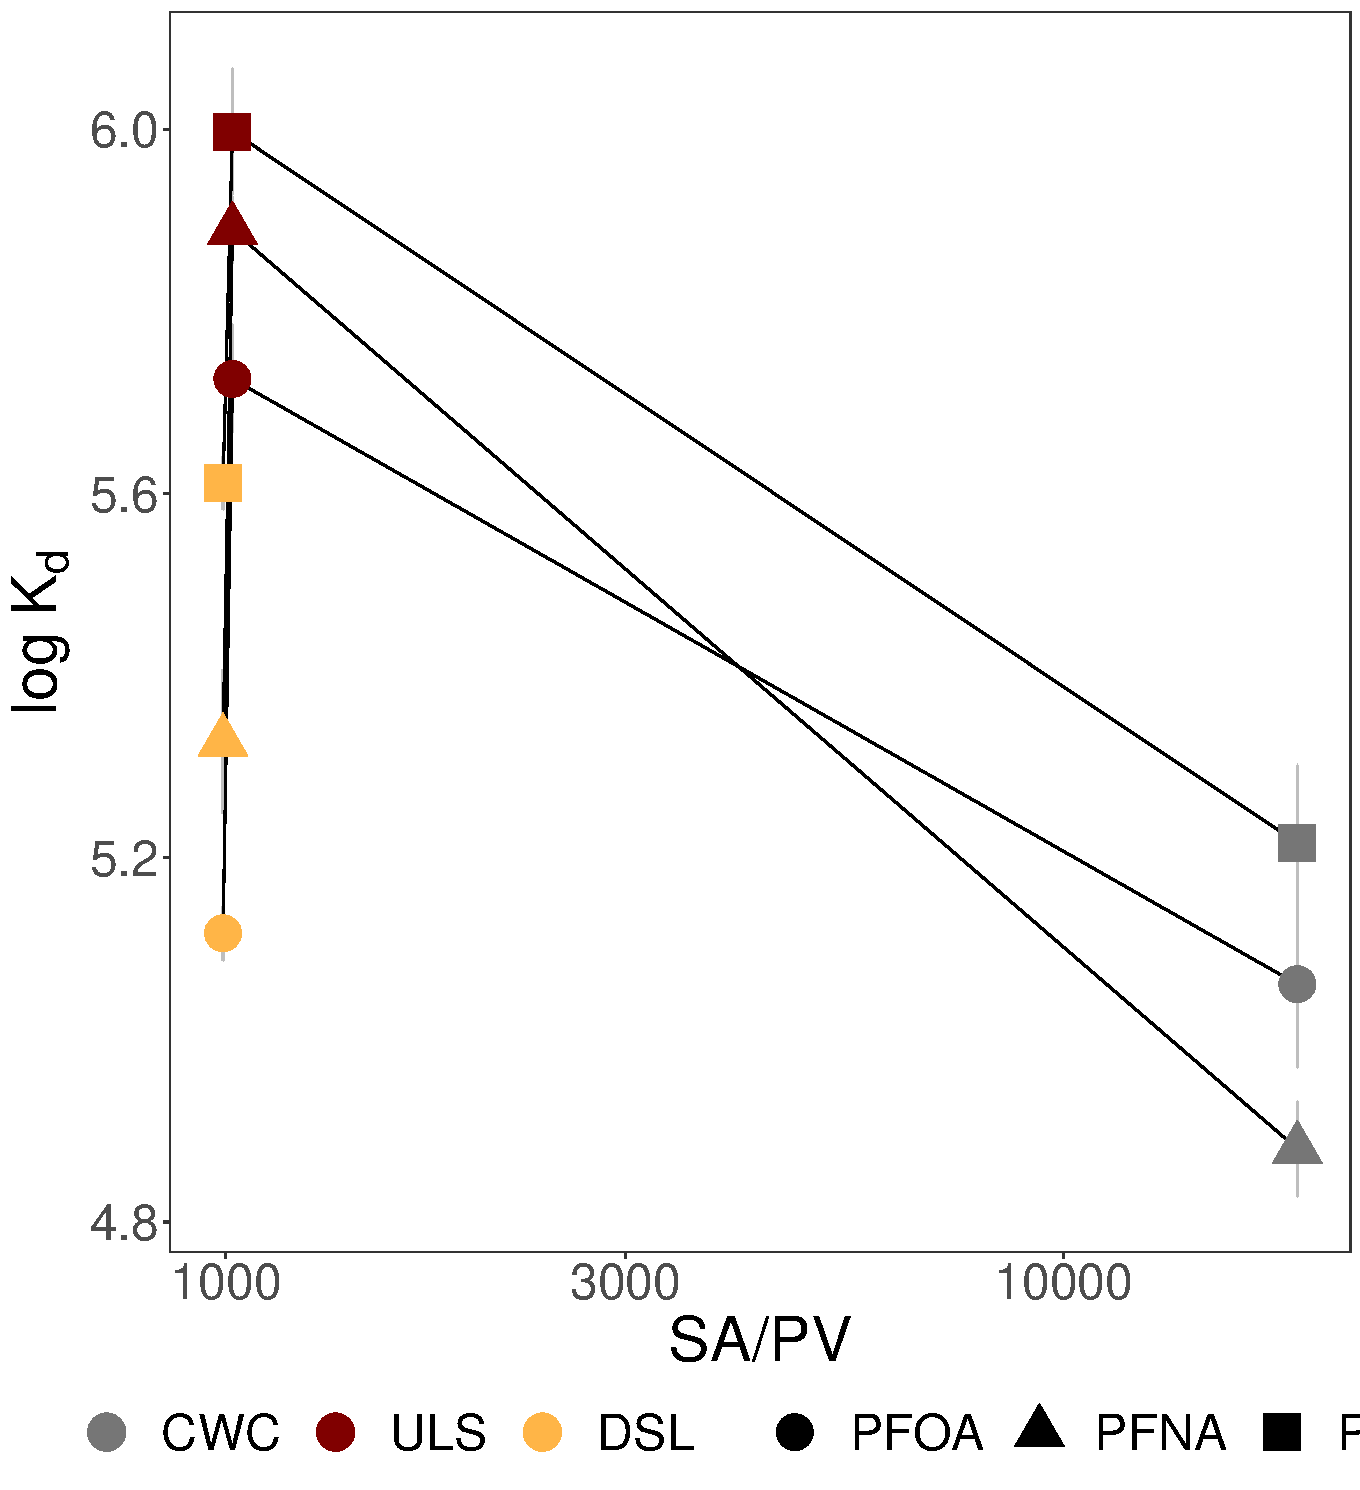
\includegraphics[width=0.3\textwidth]{R/figs/Kd_1ugL_SA_PV.pdf}
}
\hfill
\subfloat[\label{subfig:Kd_SAPVC}]{%
  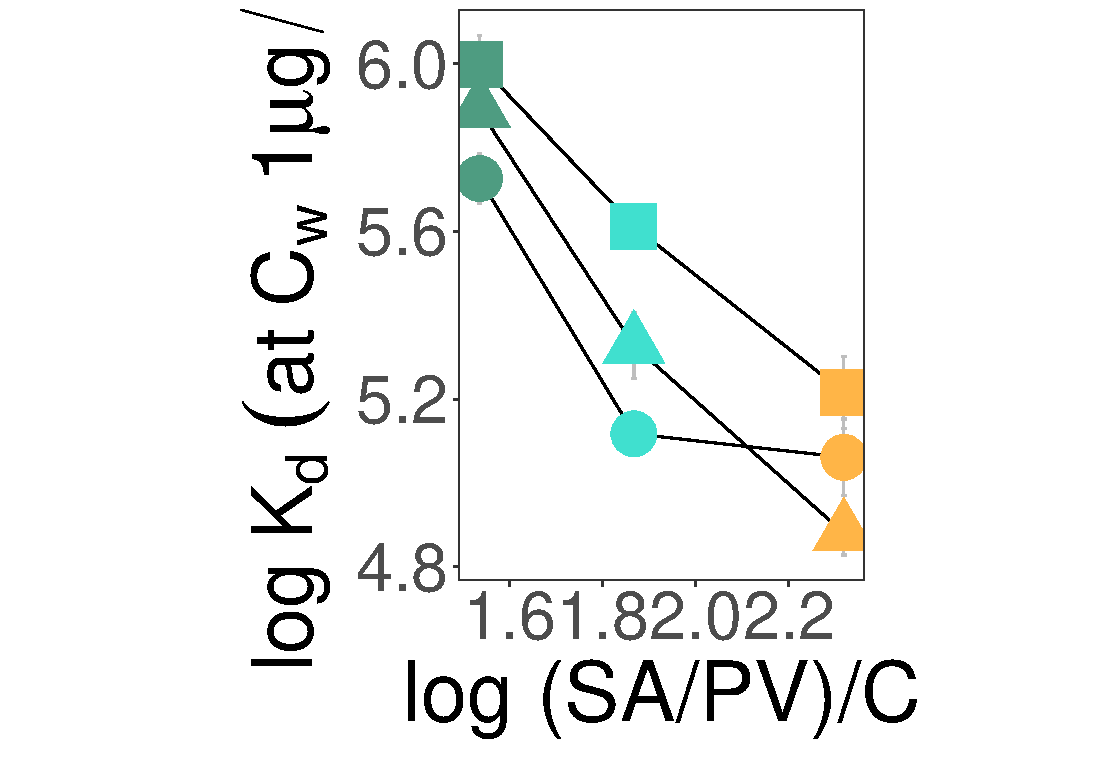
\includegraphics[width=0.3\textwidth]{R/figs/Kd_1ugL_SA_PV_C.pdf}
}
\caption{The correlation of $log~K_d$ vs. (a) log C (b) log SA/PV (c) log (SA/PV)/C using BET for SA and BJH for PV by biomass feedstock. Error bars are the propagated standard error.}
\label{fig:Kd_SAPV_C}
\end{figure}

\begin{figure}[!ht]
\subfloat[\label{subfig:Kd_Ca}]{%
  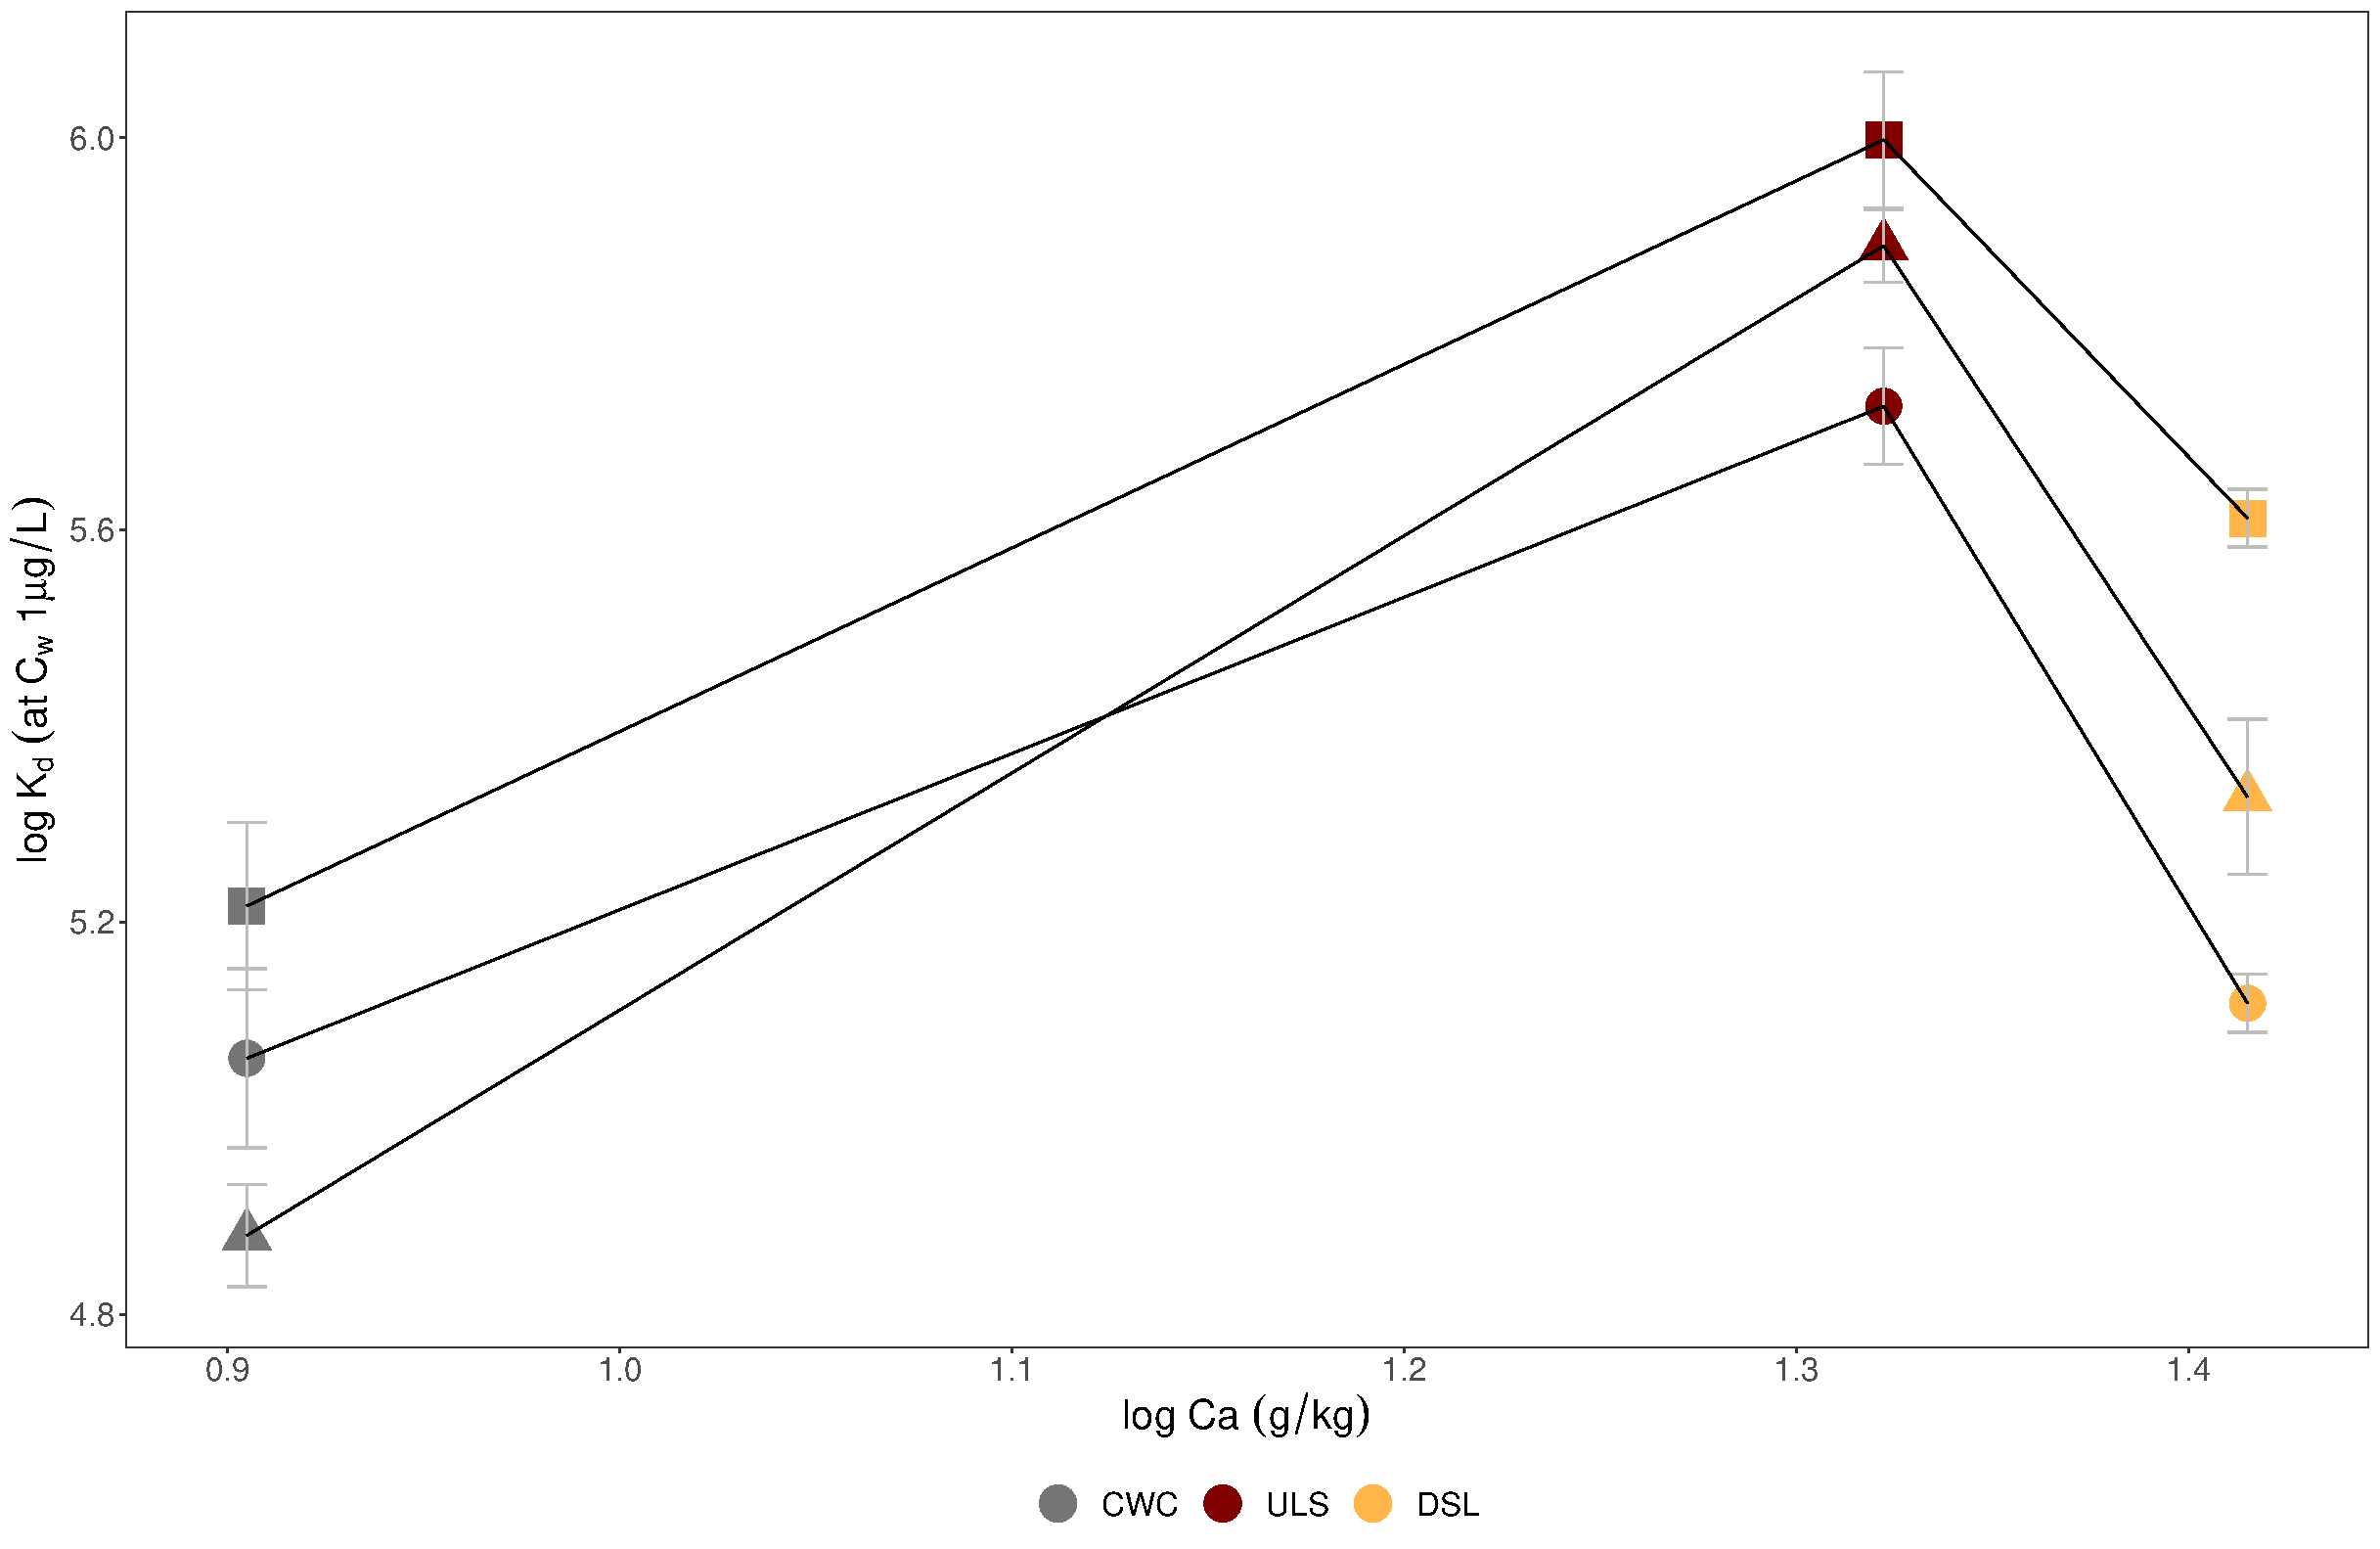
\includegraphics[width=0.45\textwidth]{R/figs/Kd_1ugL_Ca.pdf}
}
\hfill
\subfloat[\label{subfig:Kd_PV}]{%
  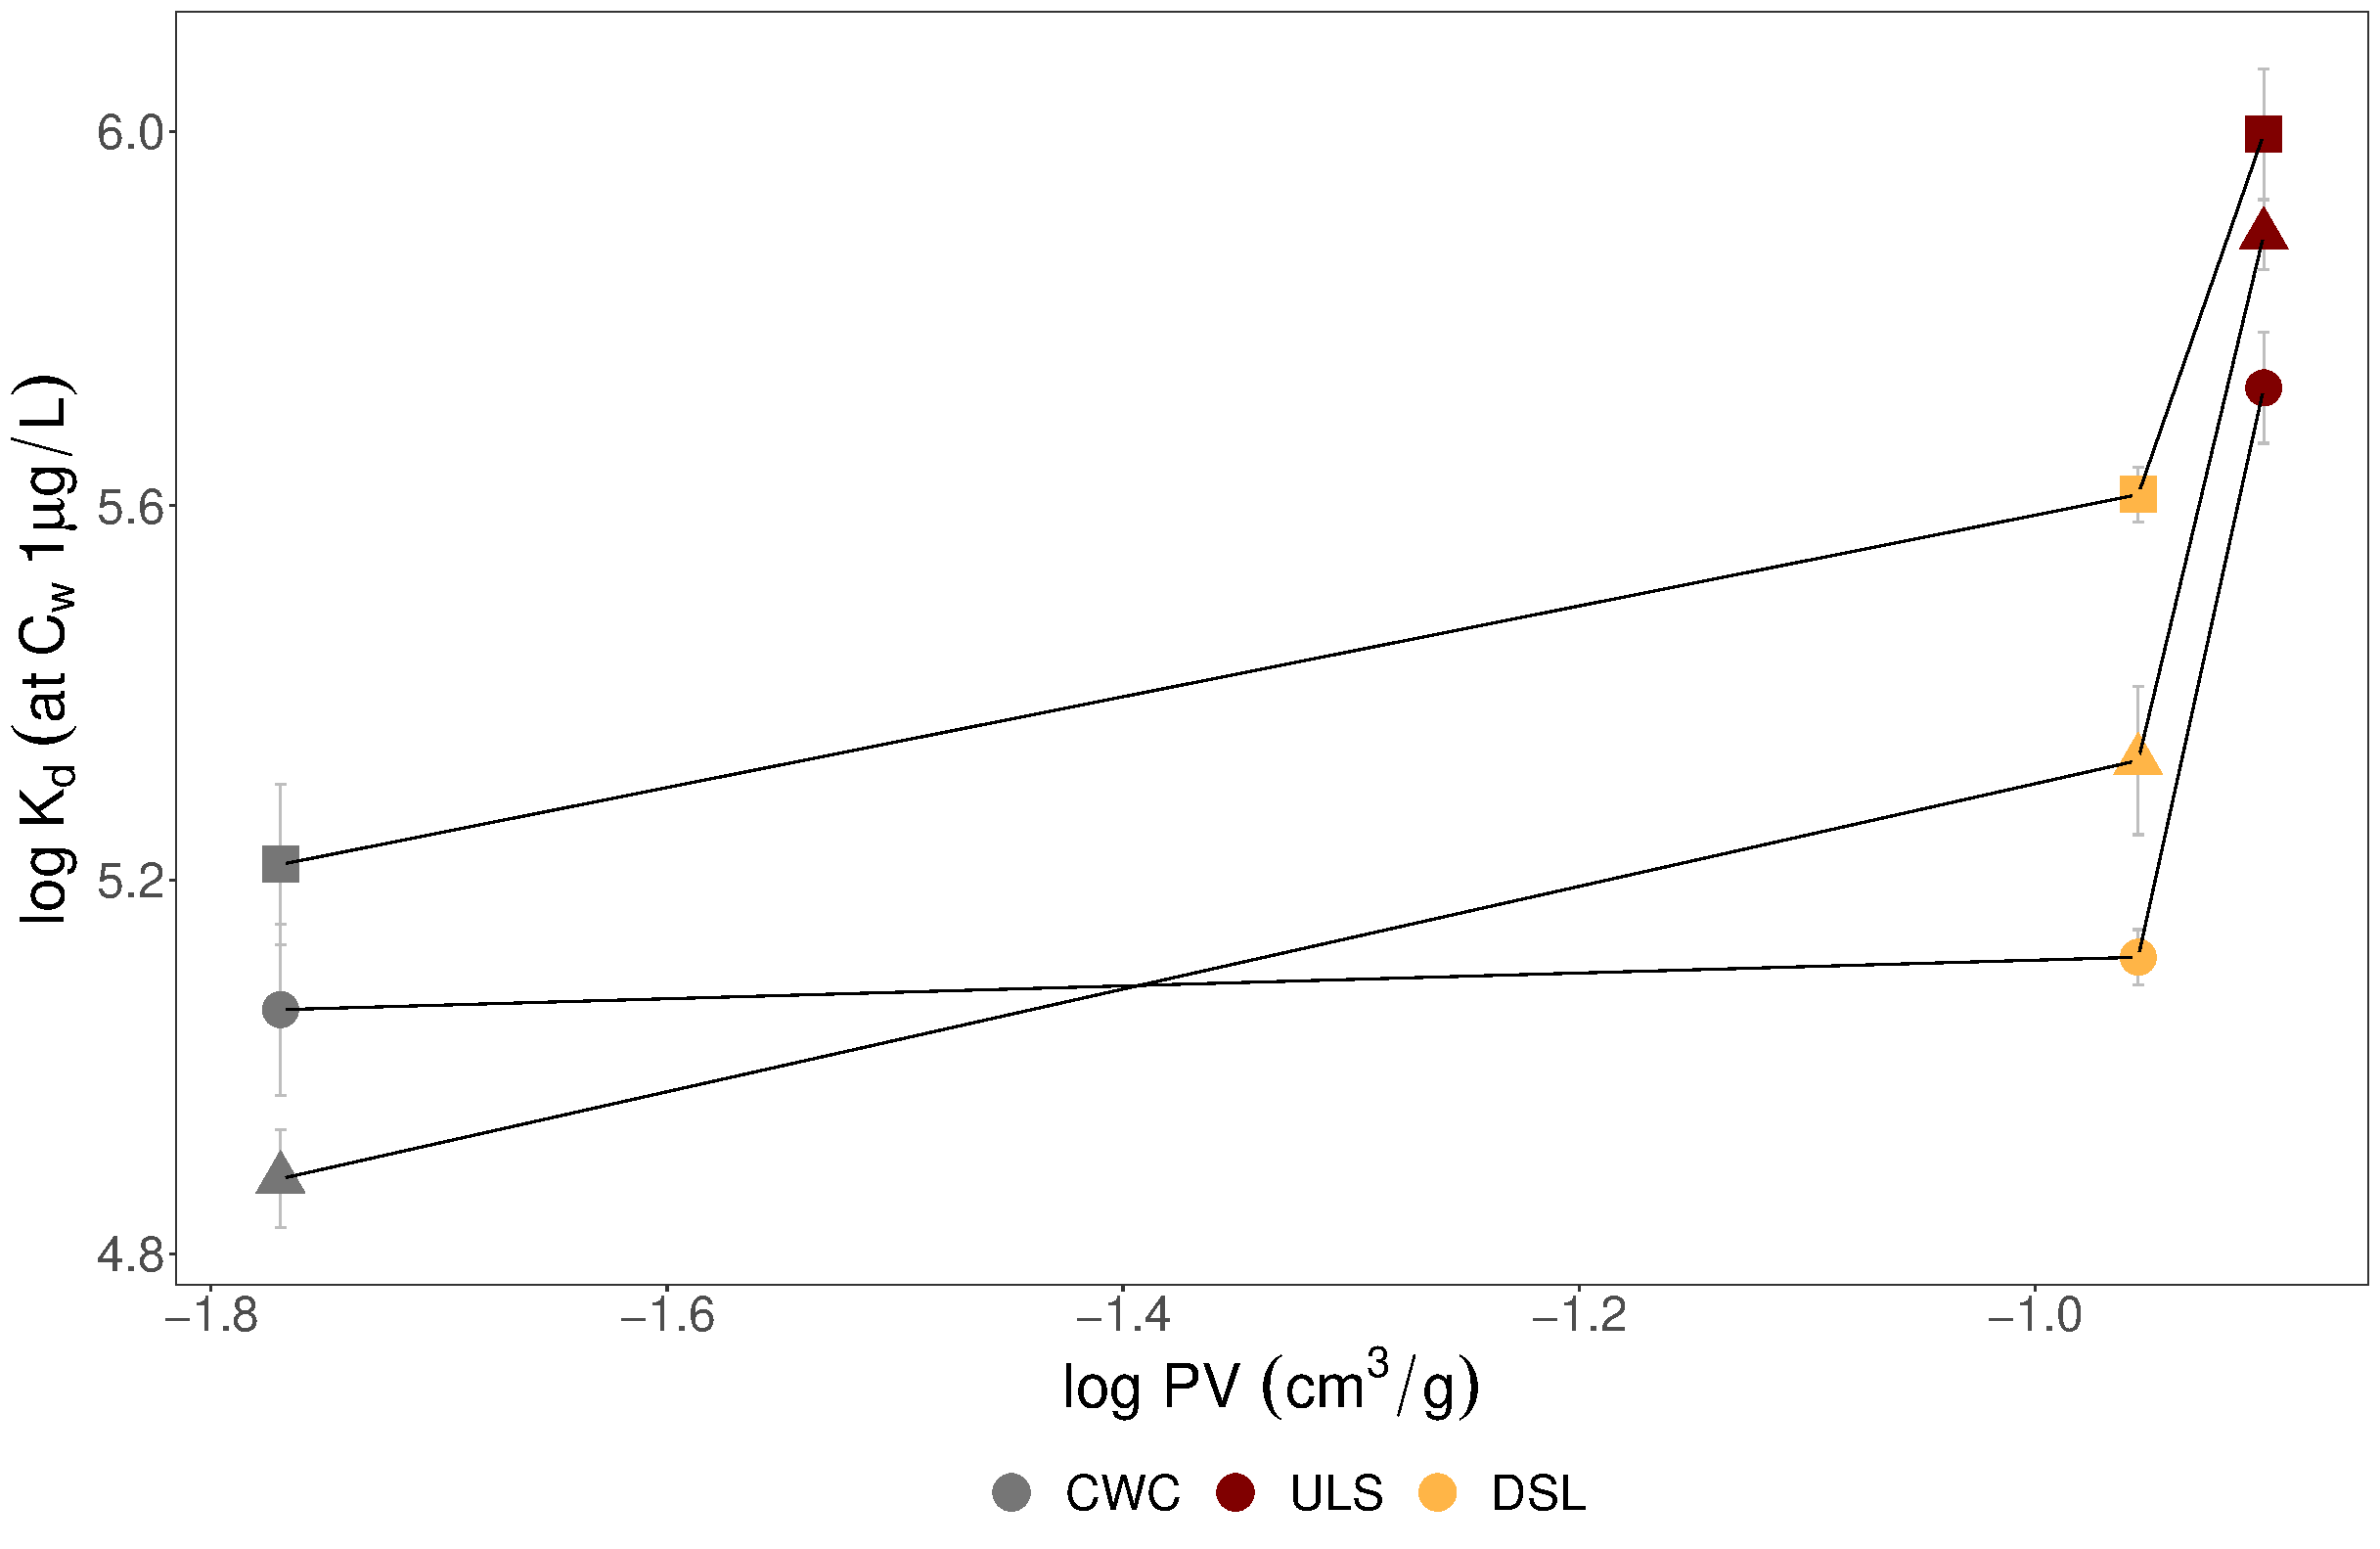
\includegraphics[width=0.45\textwidth]{R/figs/Kd_1ugL_PVN2.pdf}
}
\hfill
\subfloat[\label{subfig:Kd_PV_Ca}]{%
  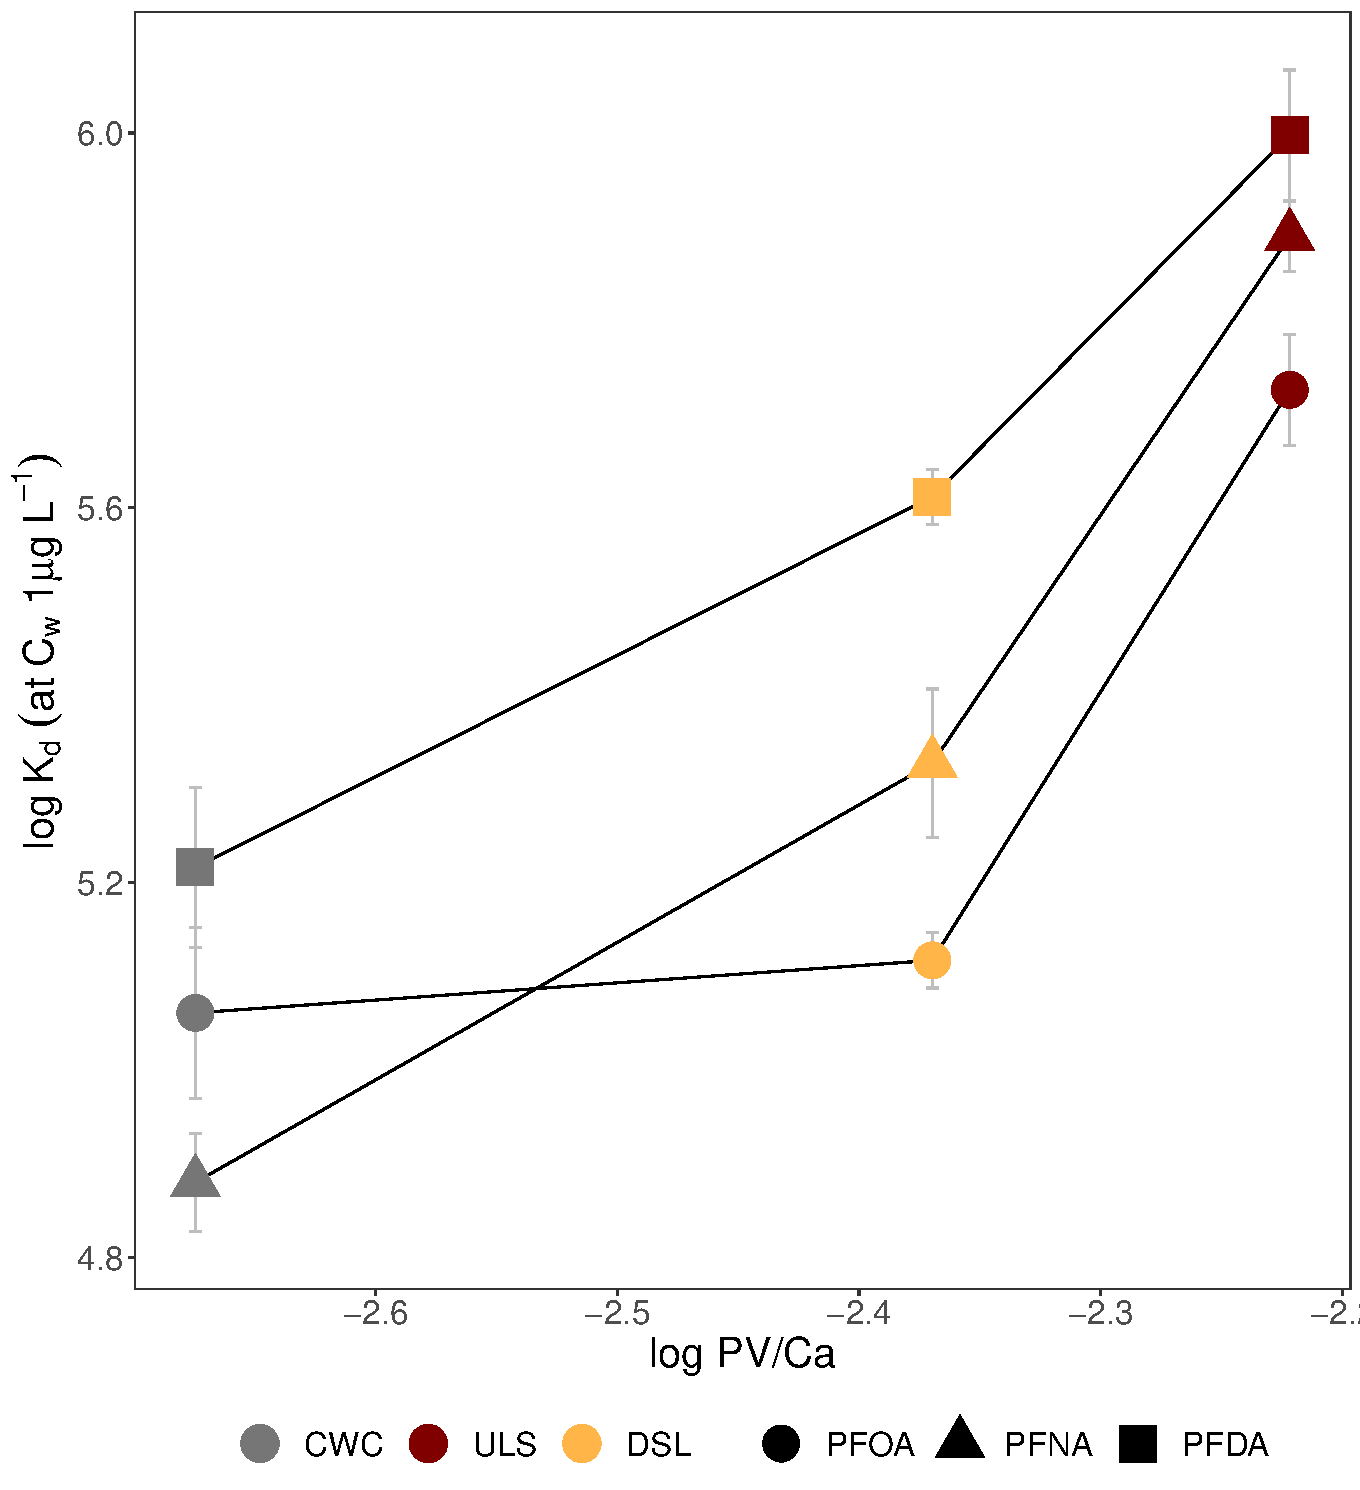
\includegraphics[width=0.45\textwidth]{R/figs/Kd_1ugL_PVN2_Ca.pdf}
}
\hfill
\subfloat[\label{subfig:Kd_SAPVCa}]{%
  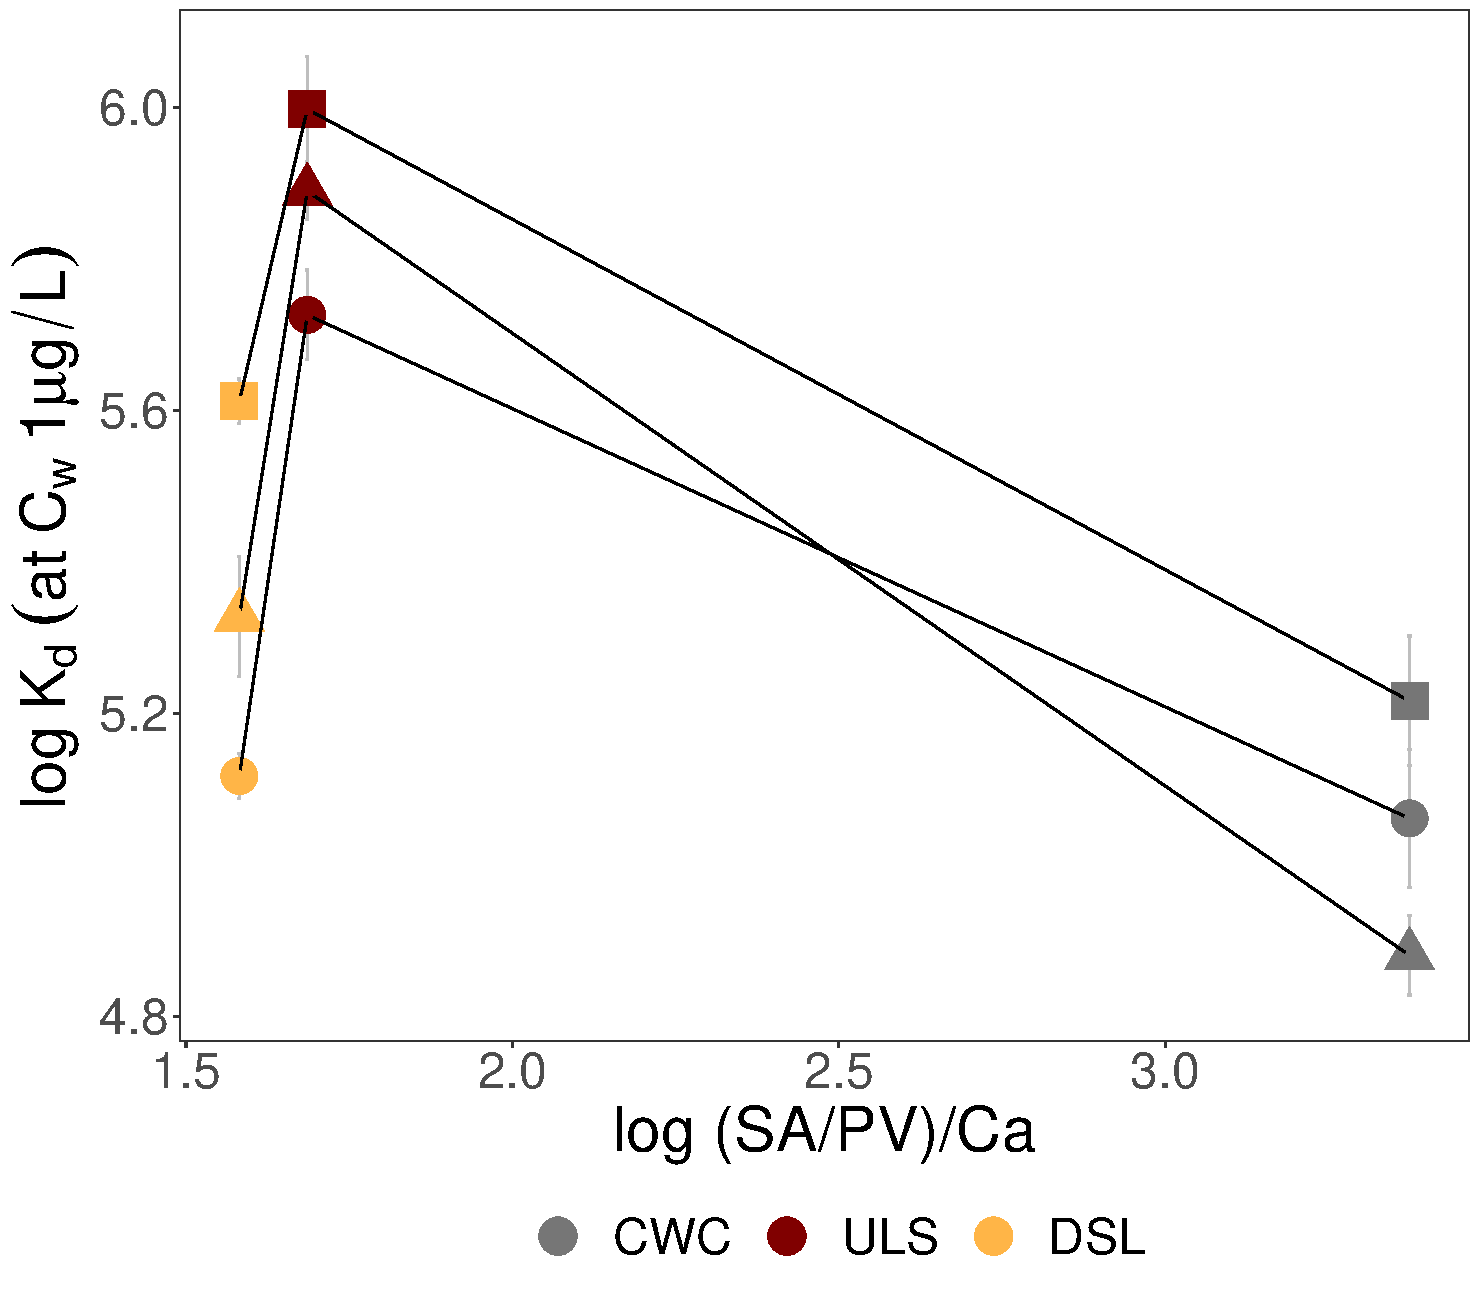
\includegraphics[width=0.45\textwidth]{R/figs/Kd_1ugL_SA_PV_Ca.pdf}
}
\caption{The correlation of $log~K_d$ vs. (a) log Ca (b) log PV (c) log PV/Ca (d) log (SA/PV)/Ca using BET for SA and BJH for PV by biomass feedstock. Error bars are the propagated standard error.}
\label{fig:Kd_SAPV_Ca}
\end{figure}

\begin{figure}[!ht]
\subfloat[\label{subfig:SA_small}]{%
  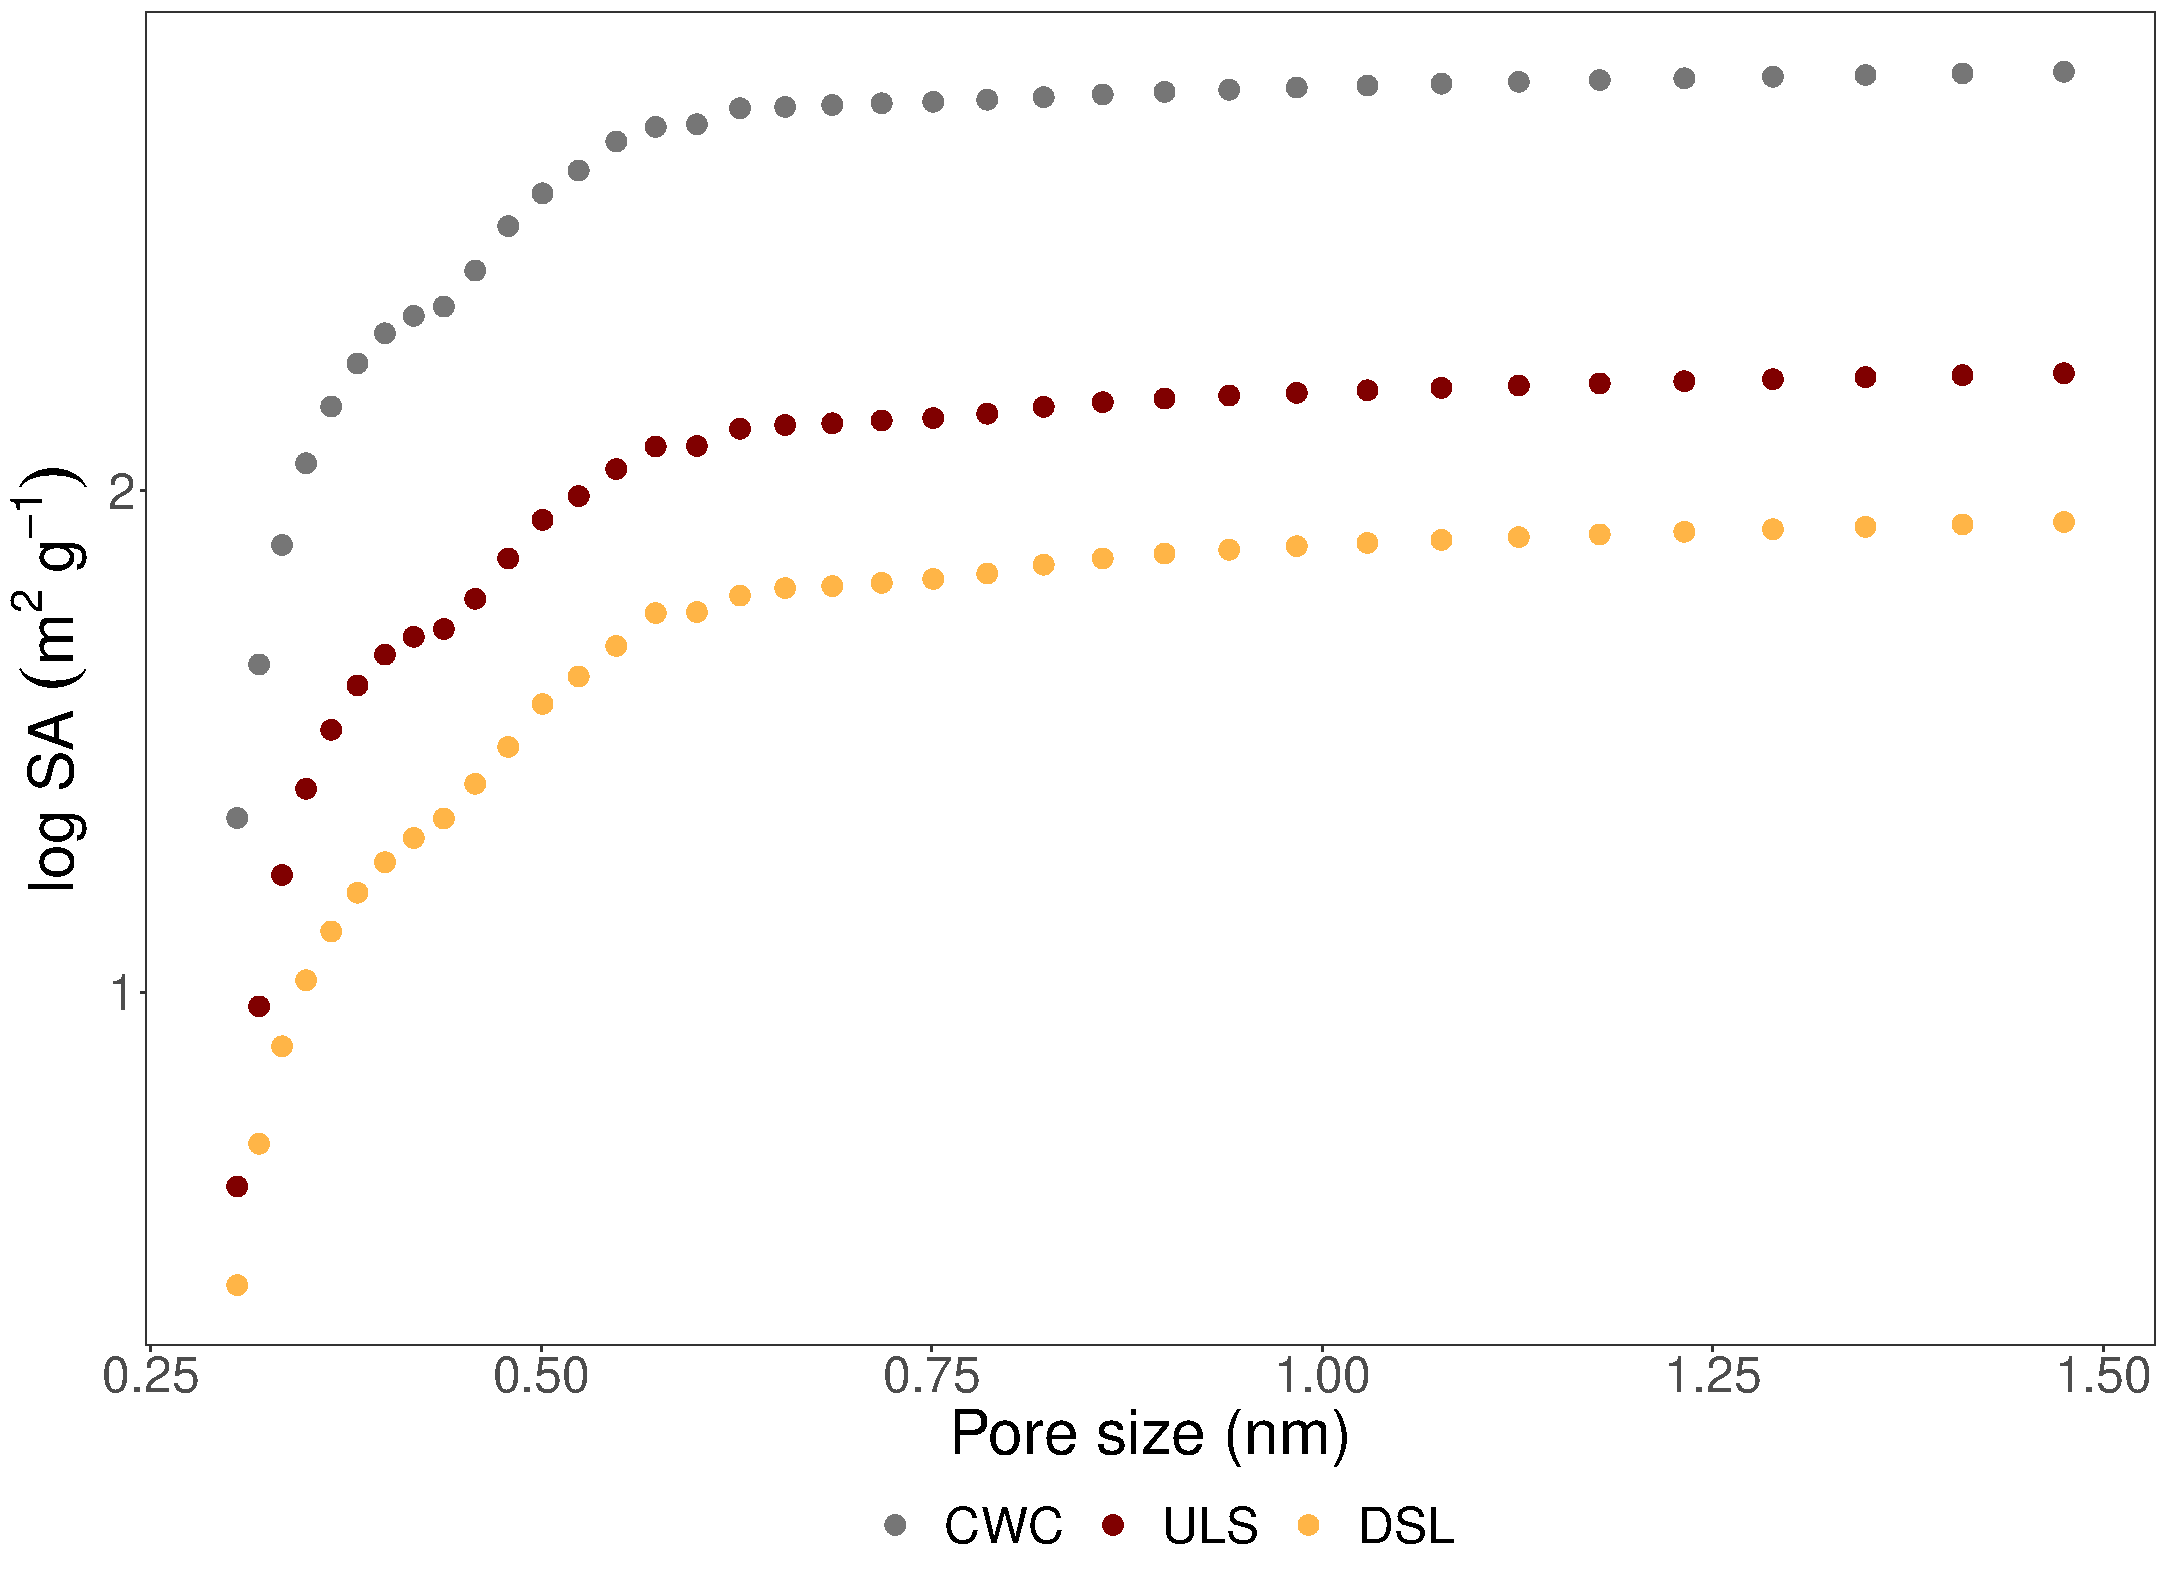
\includegraphics[width=0.31\textwidth]{R/figs/SA_small.pdf}
}
\hfill
\subfloat[\label{subfig:PV_small}]{%
  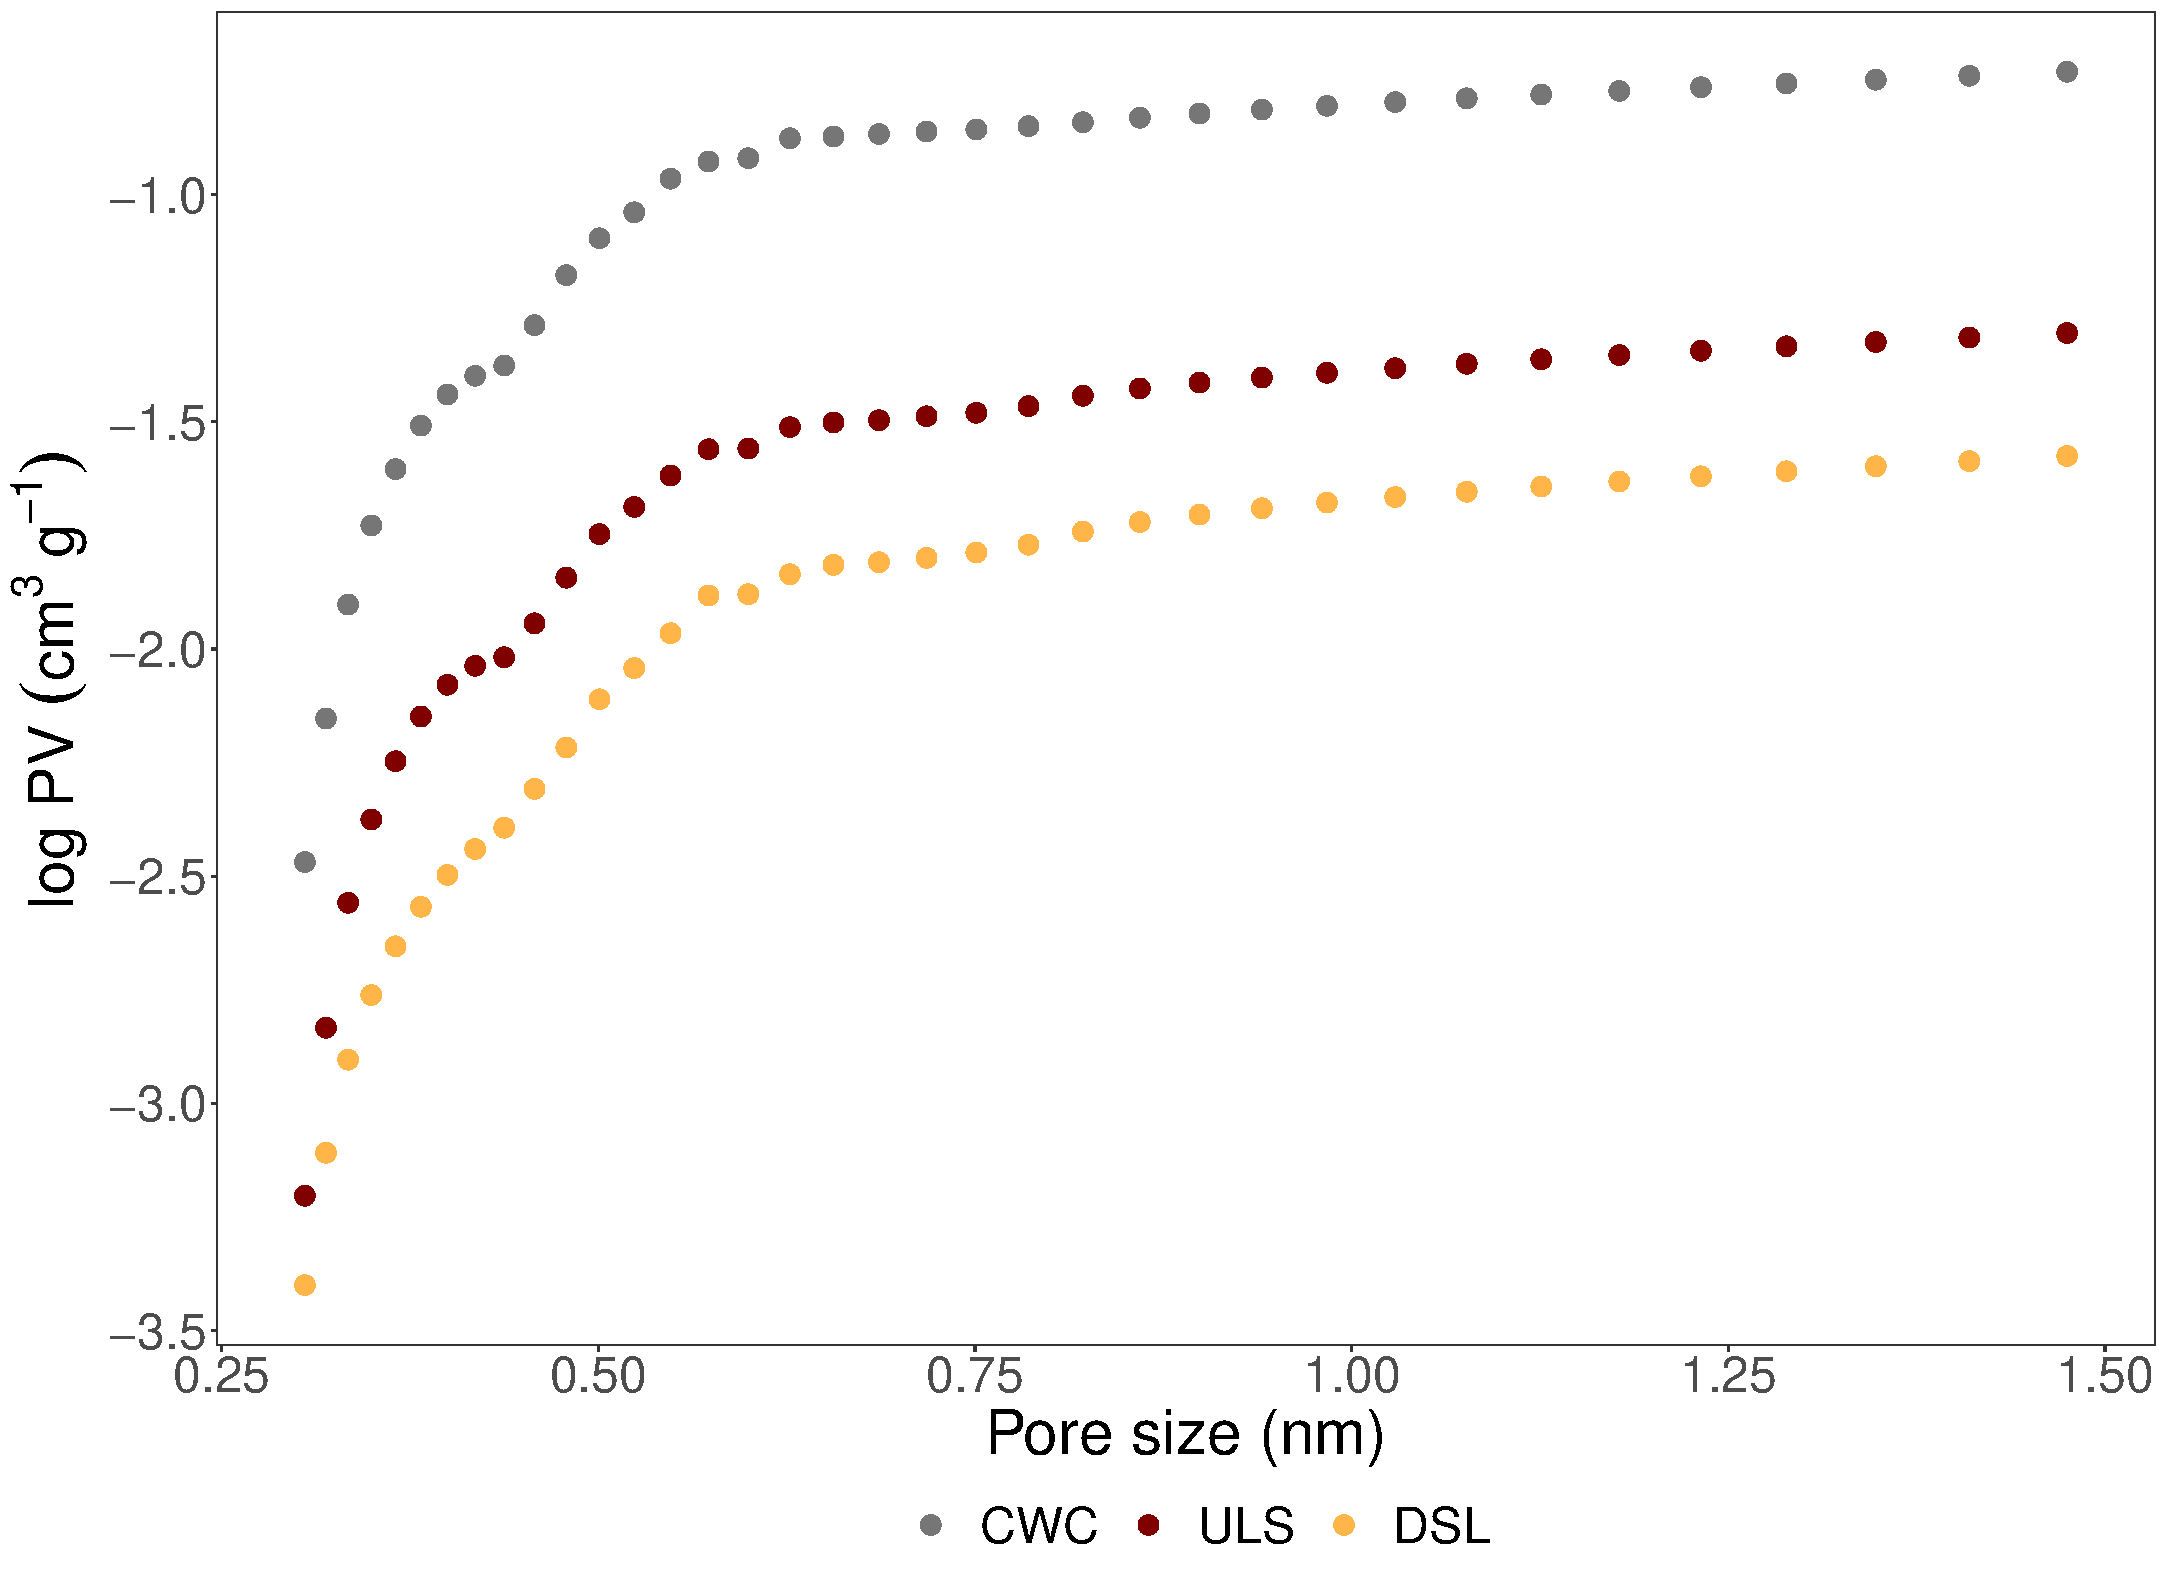
\includegraphics[width=0.31\textwidth]{R/figs/PV_small.pdf}
}
\hfill
\subfloat[\label{subfig:SAPV_small}]{%
  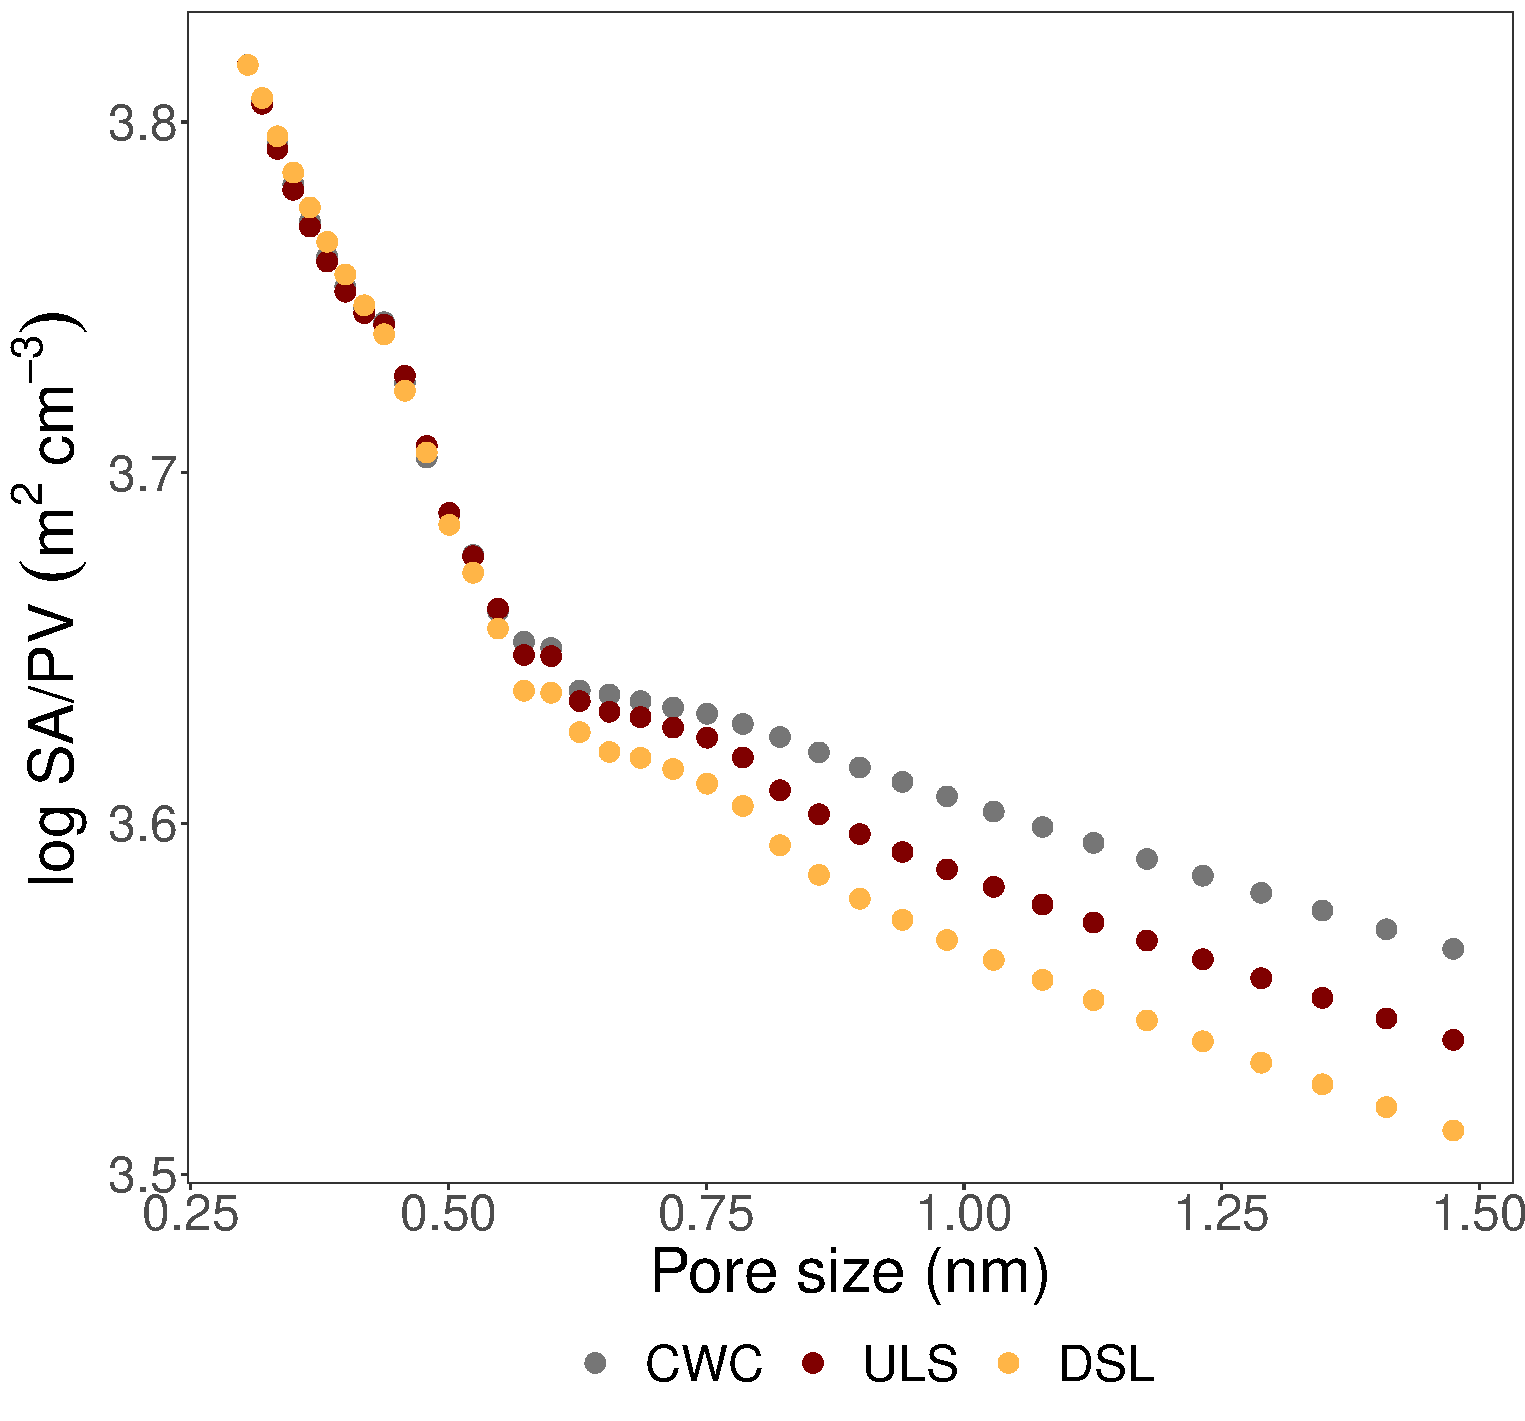
\includegraphics[width=0.31\textwidth]{R/figs/SAPV_small.pdf}
}
\caption{Cumulative pore size distribution for pores 0.4-1.5 nm using DFT.}
\label{fig:PZD_small}
\end{figure}

\begin{figure}[!ht]
\subfloat[\label{subfig:SA_large}]{%
  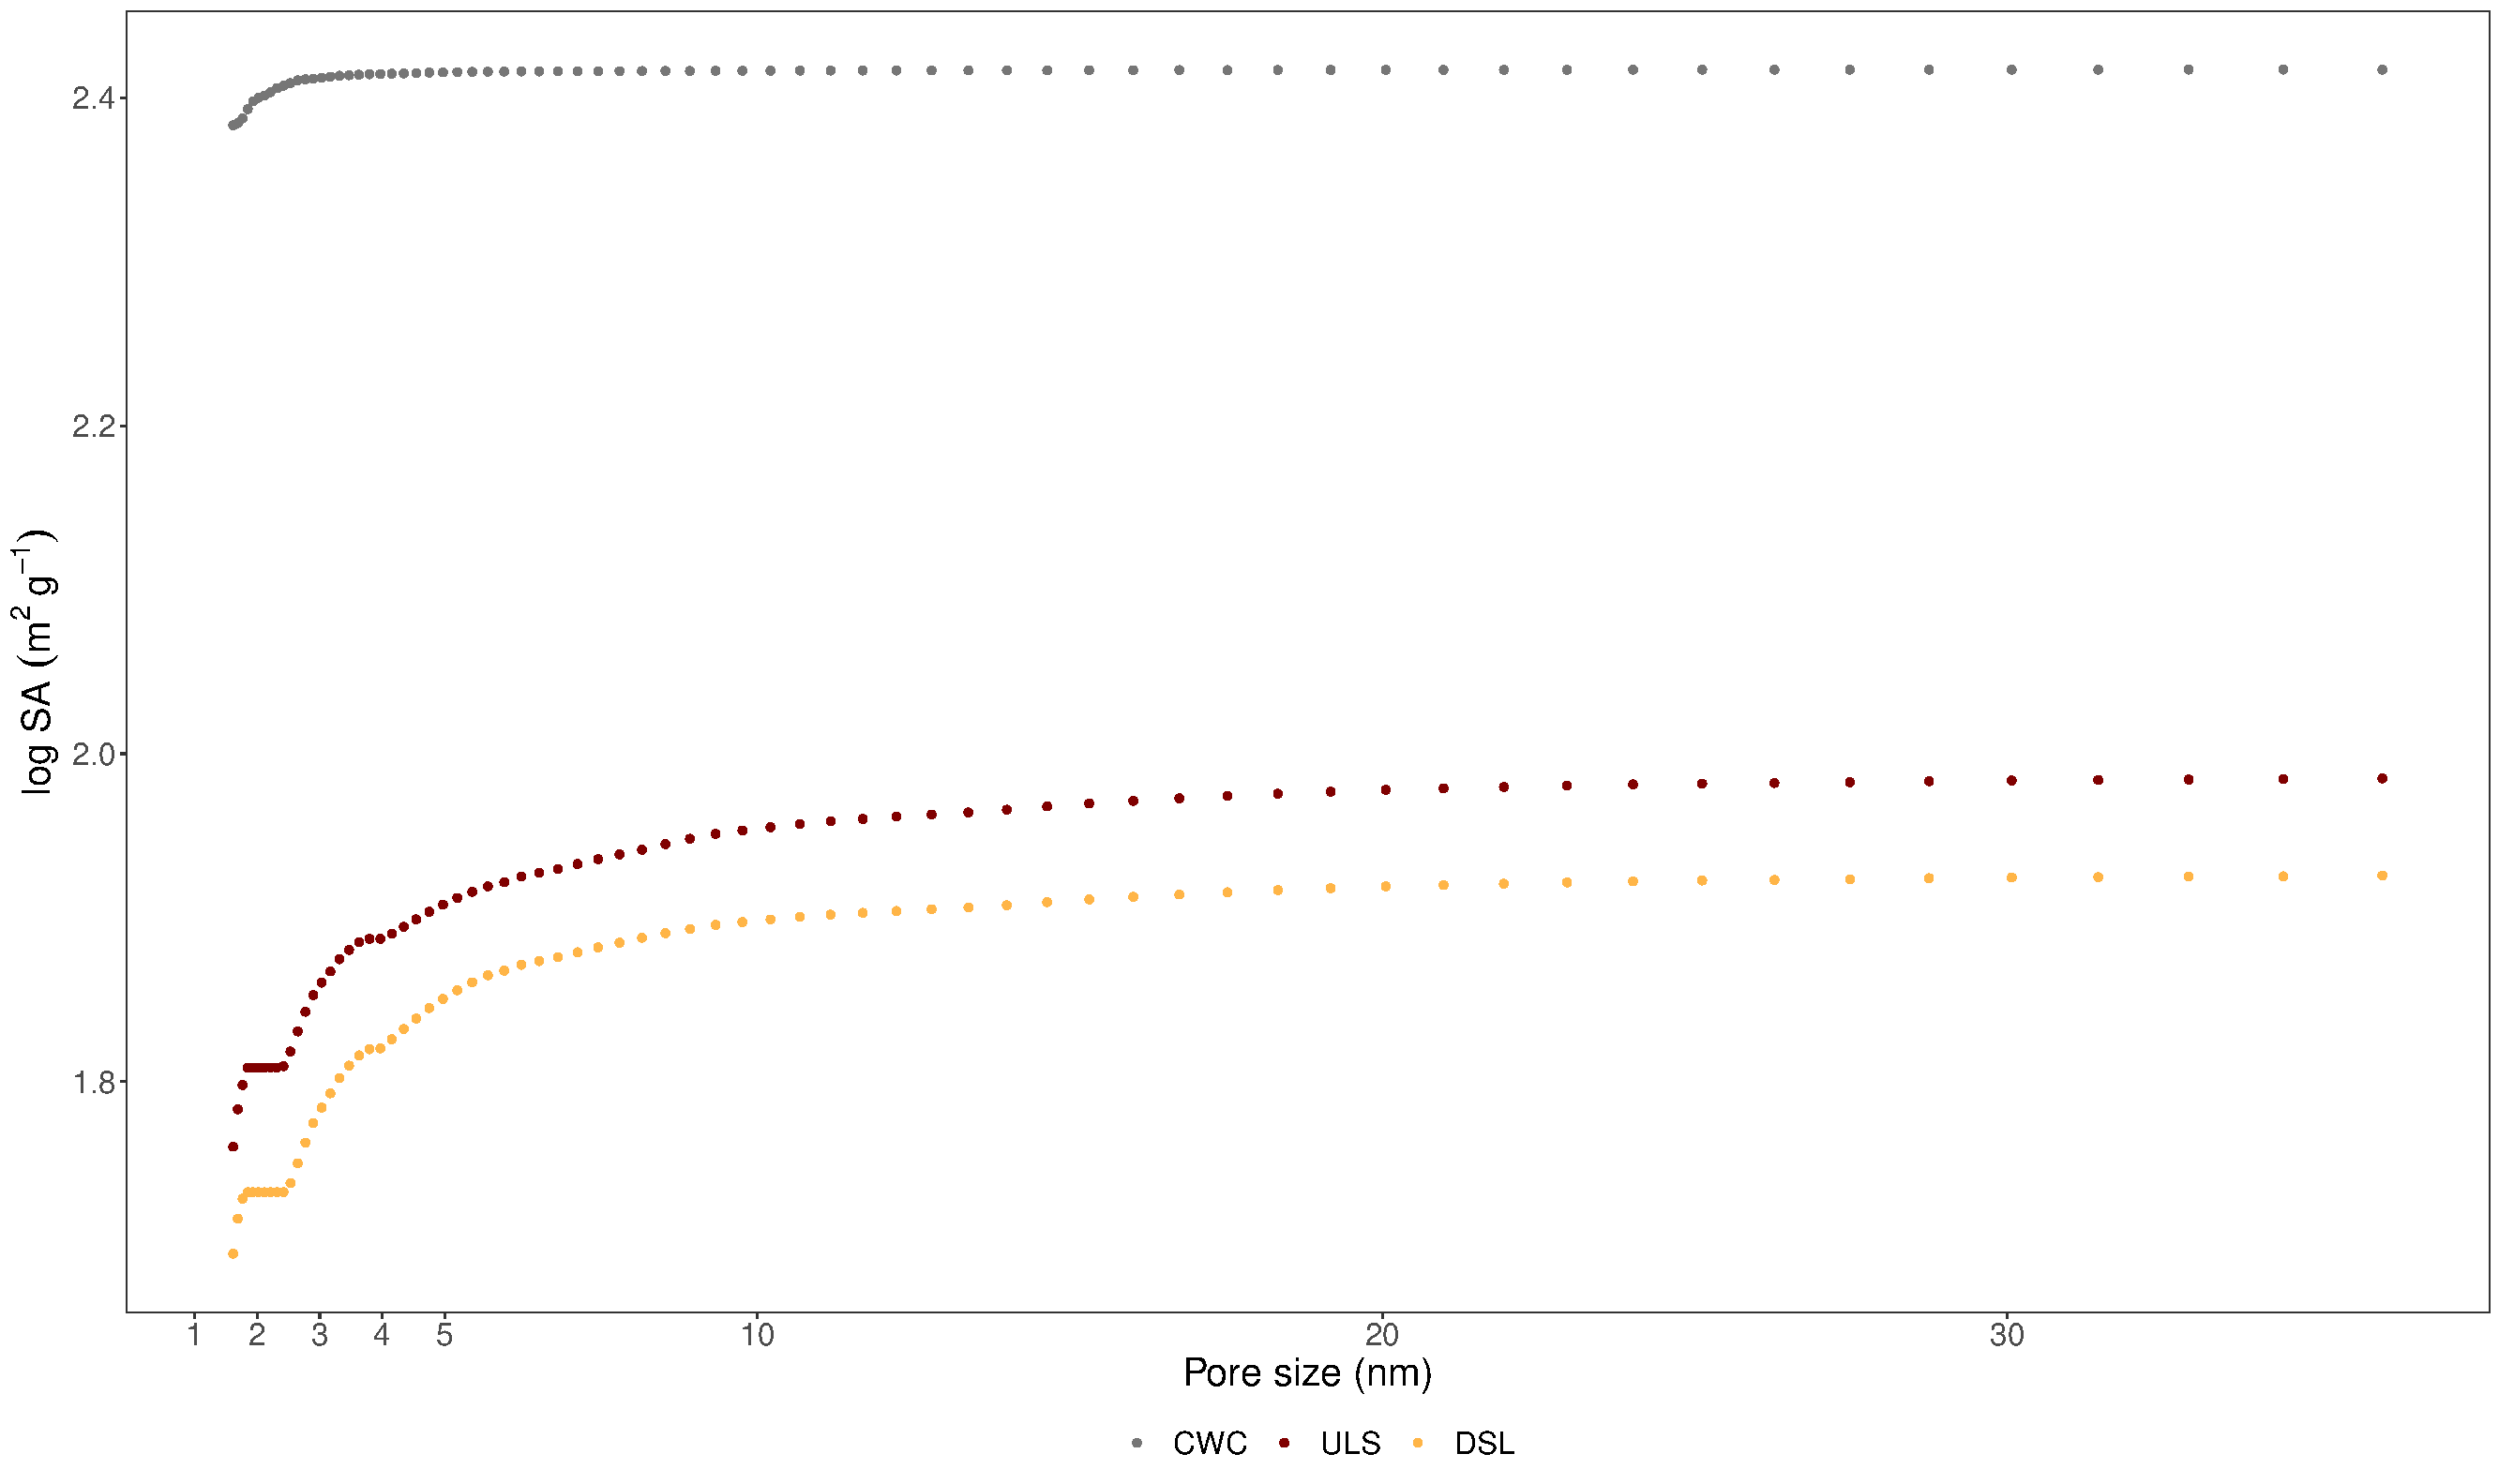
\includegraphics[width=0.45\textwidth]{R/figs/SA_large.pdf}
}
\hfill
\subfloat[\label{subfig:PV_large}]{%
  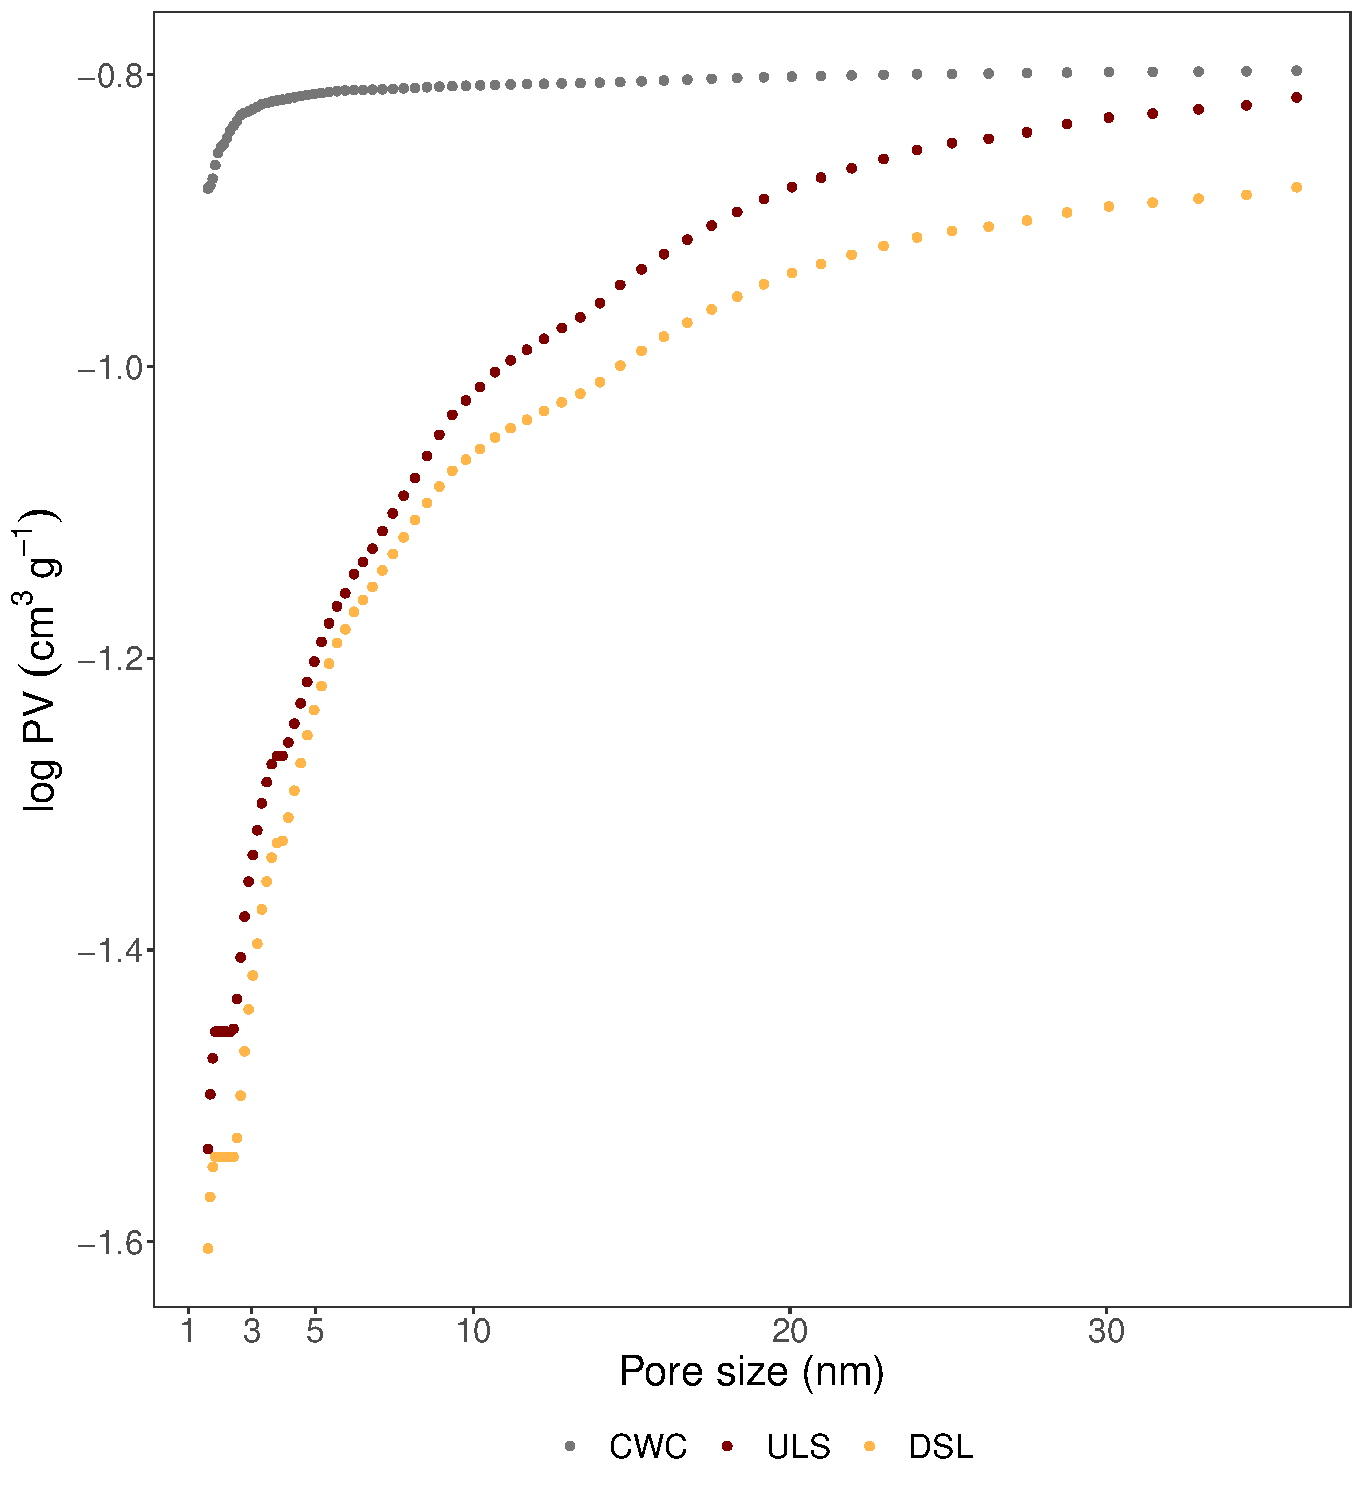
\includegraphics[width=0.45\textwidth]{R/figs/PV_large.pdf}
}
\hfill
\subfloat[\label{subfig:SAPV_large}]{%
  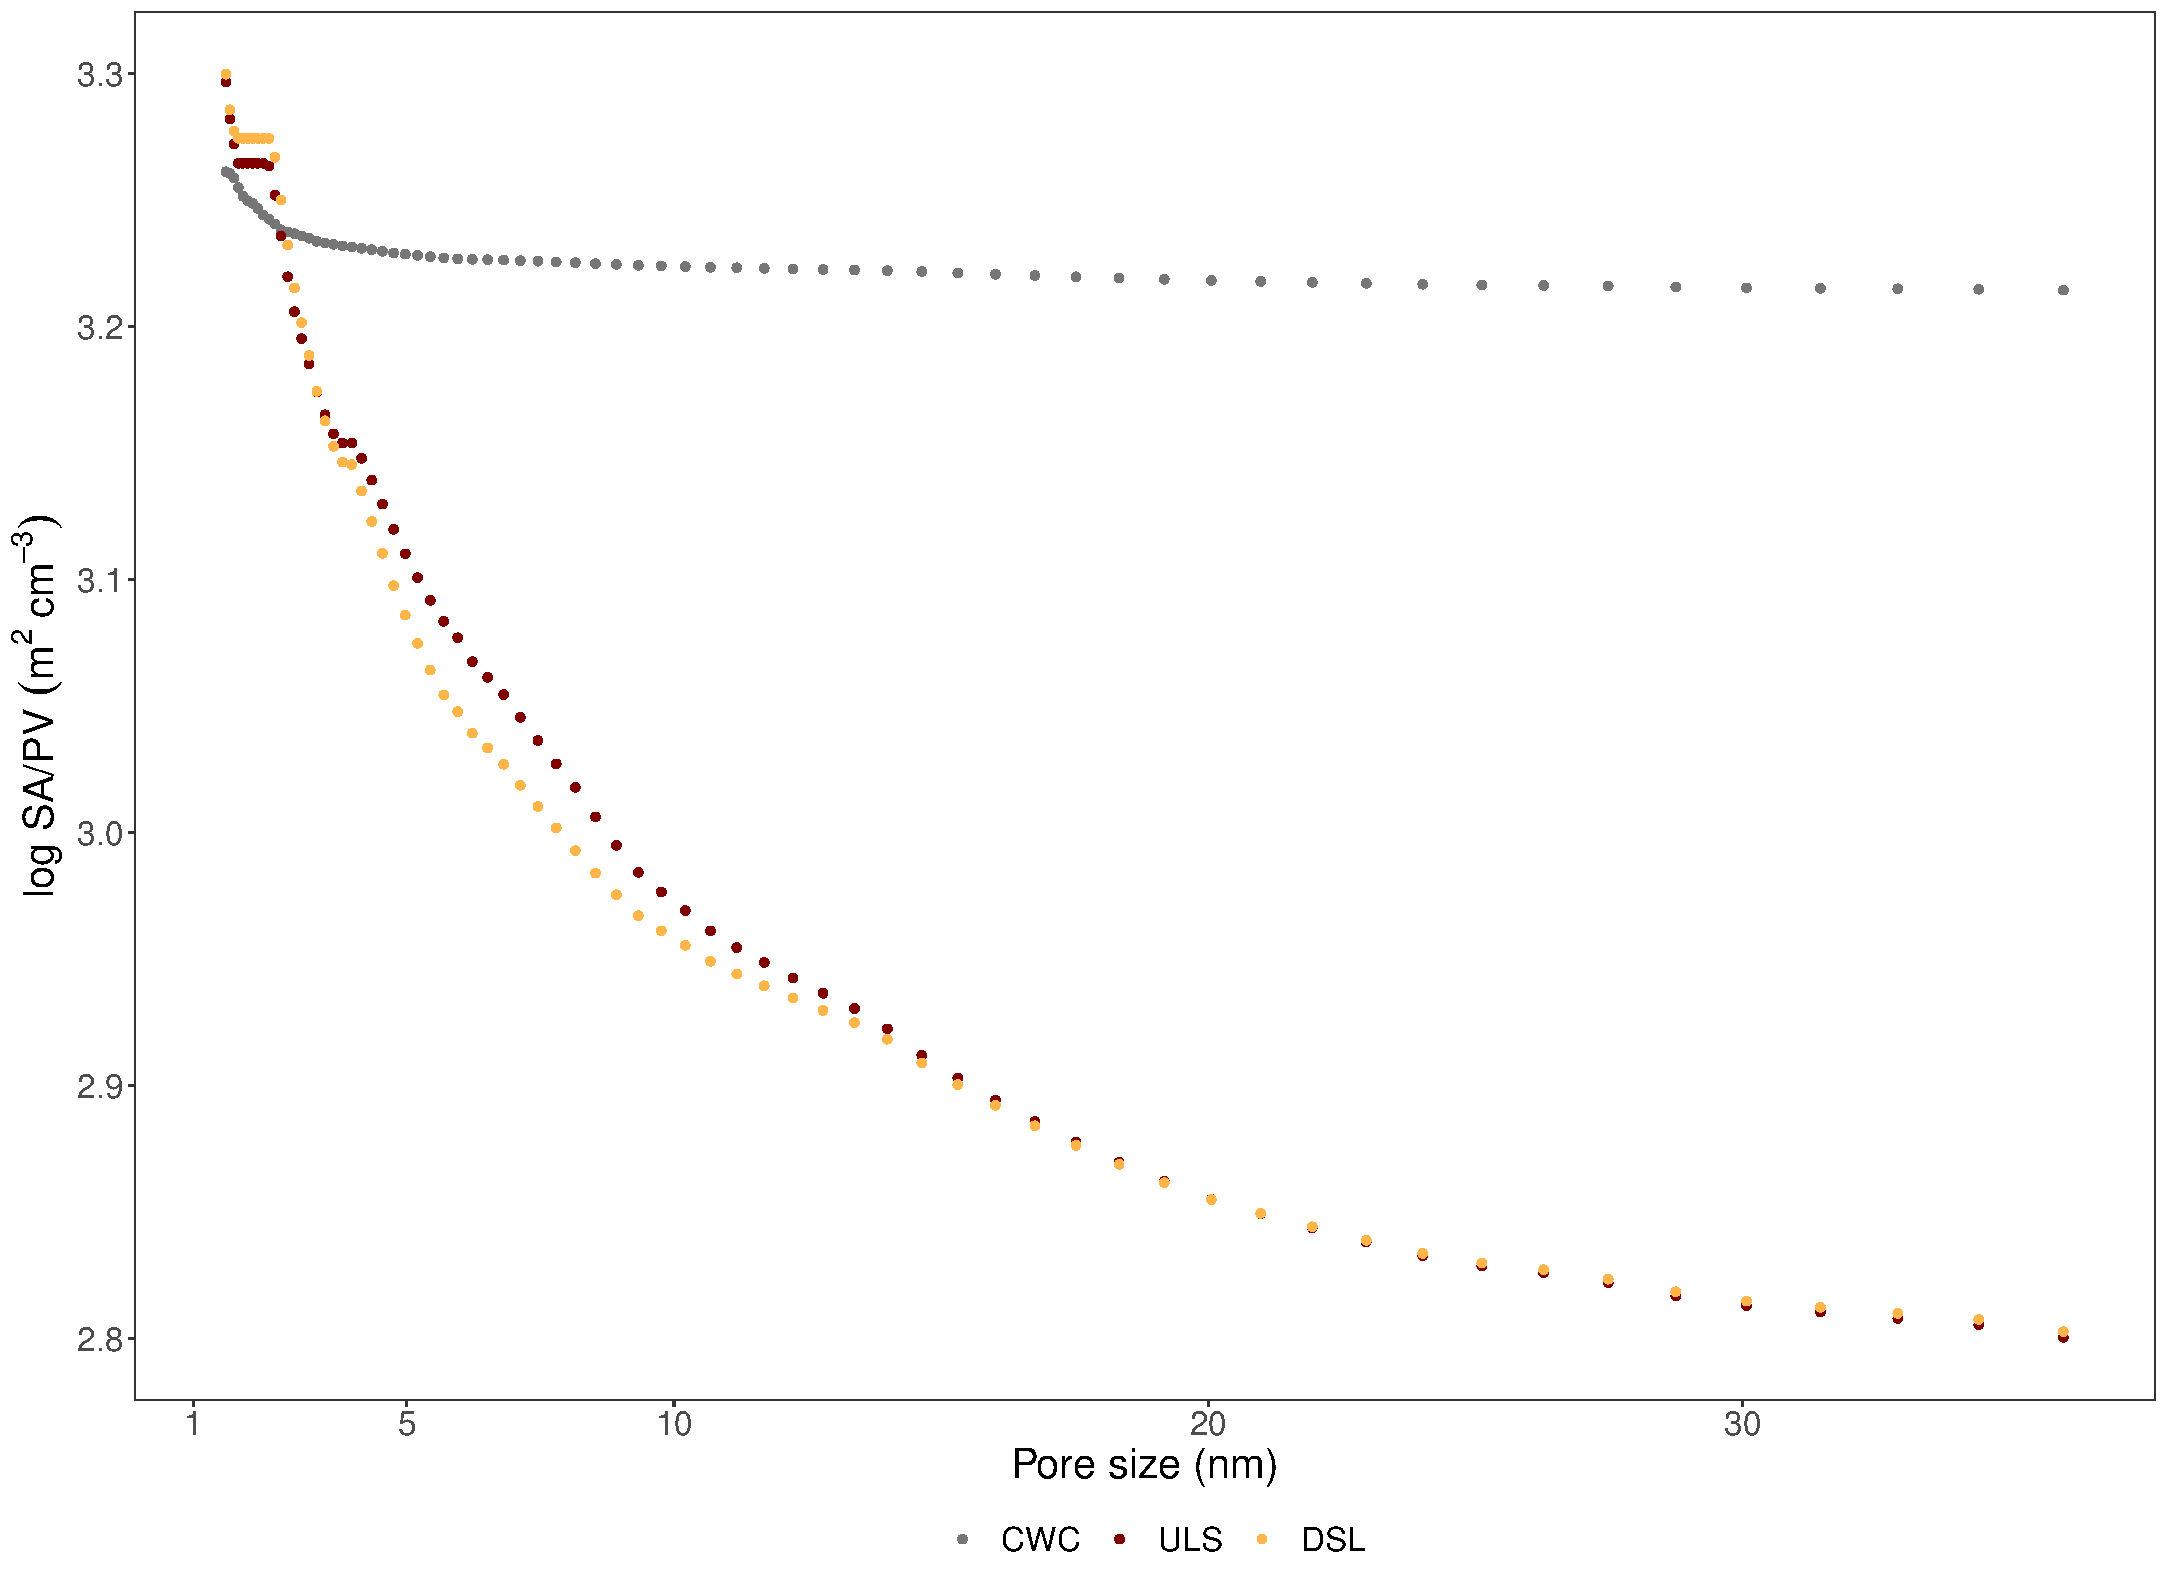
\includegraphics[width=0.45\textwidth]{R/figs/SAPV_large.pdf}
}
\hfill
\subfloat[\label{subfig:SAPV_C_large}]{%
  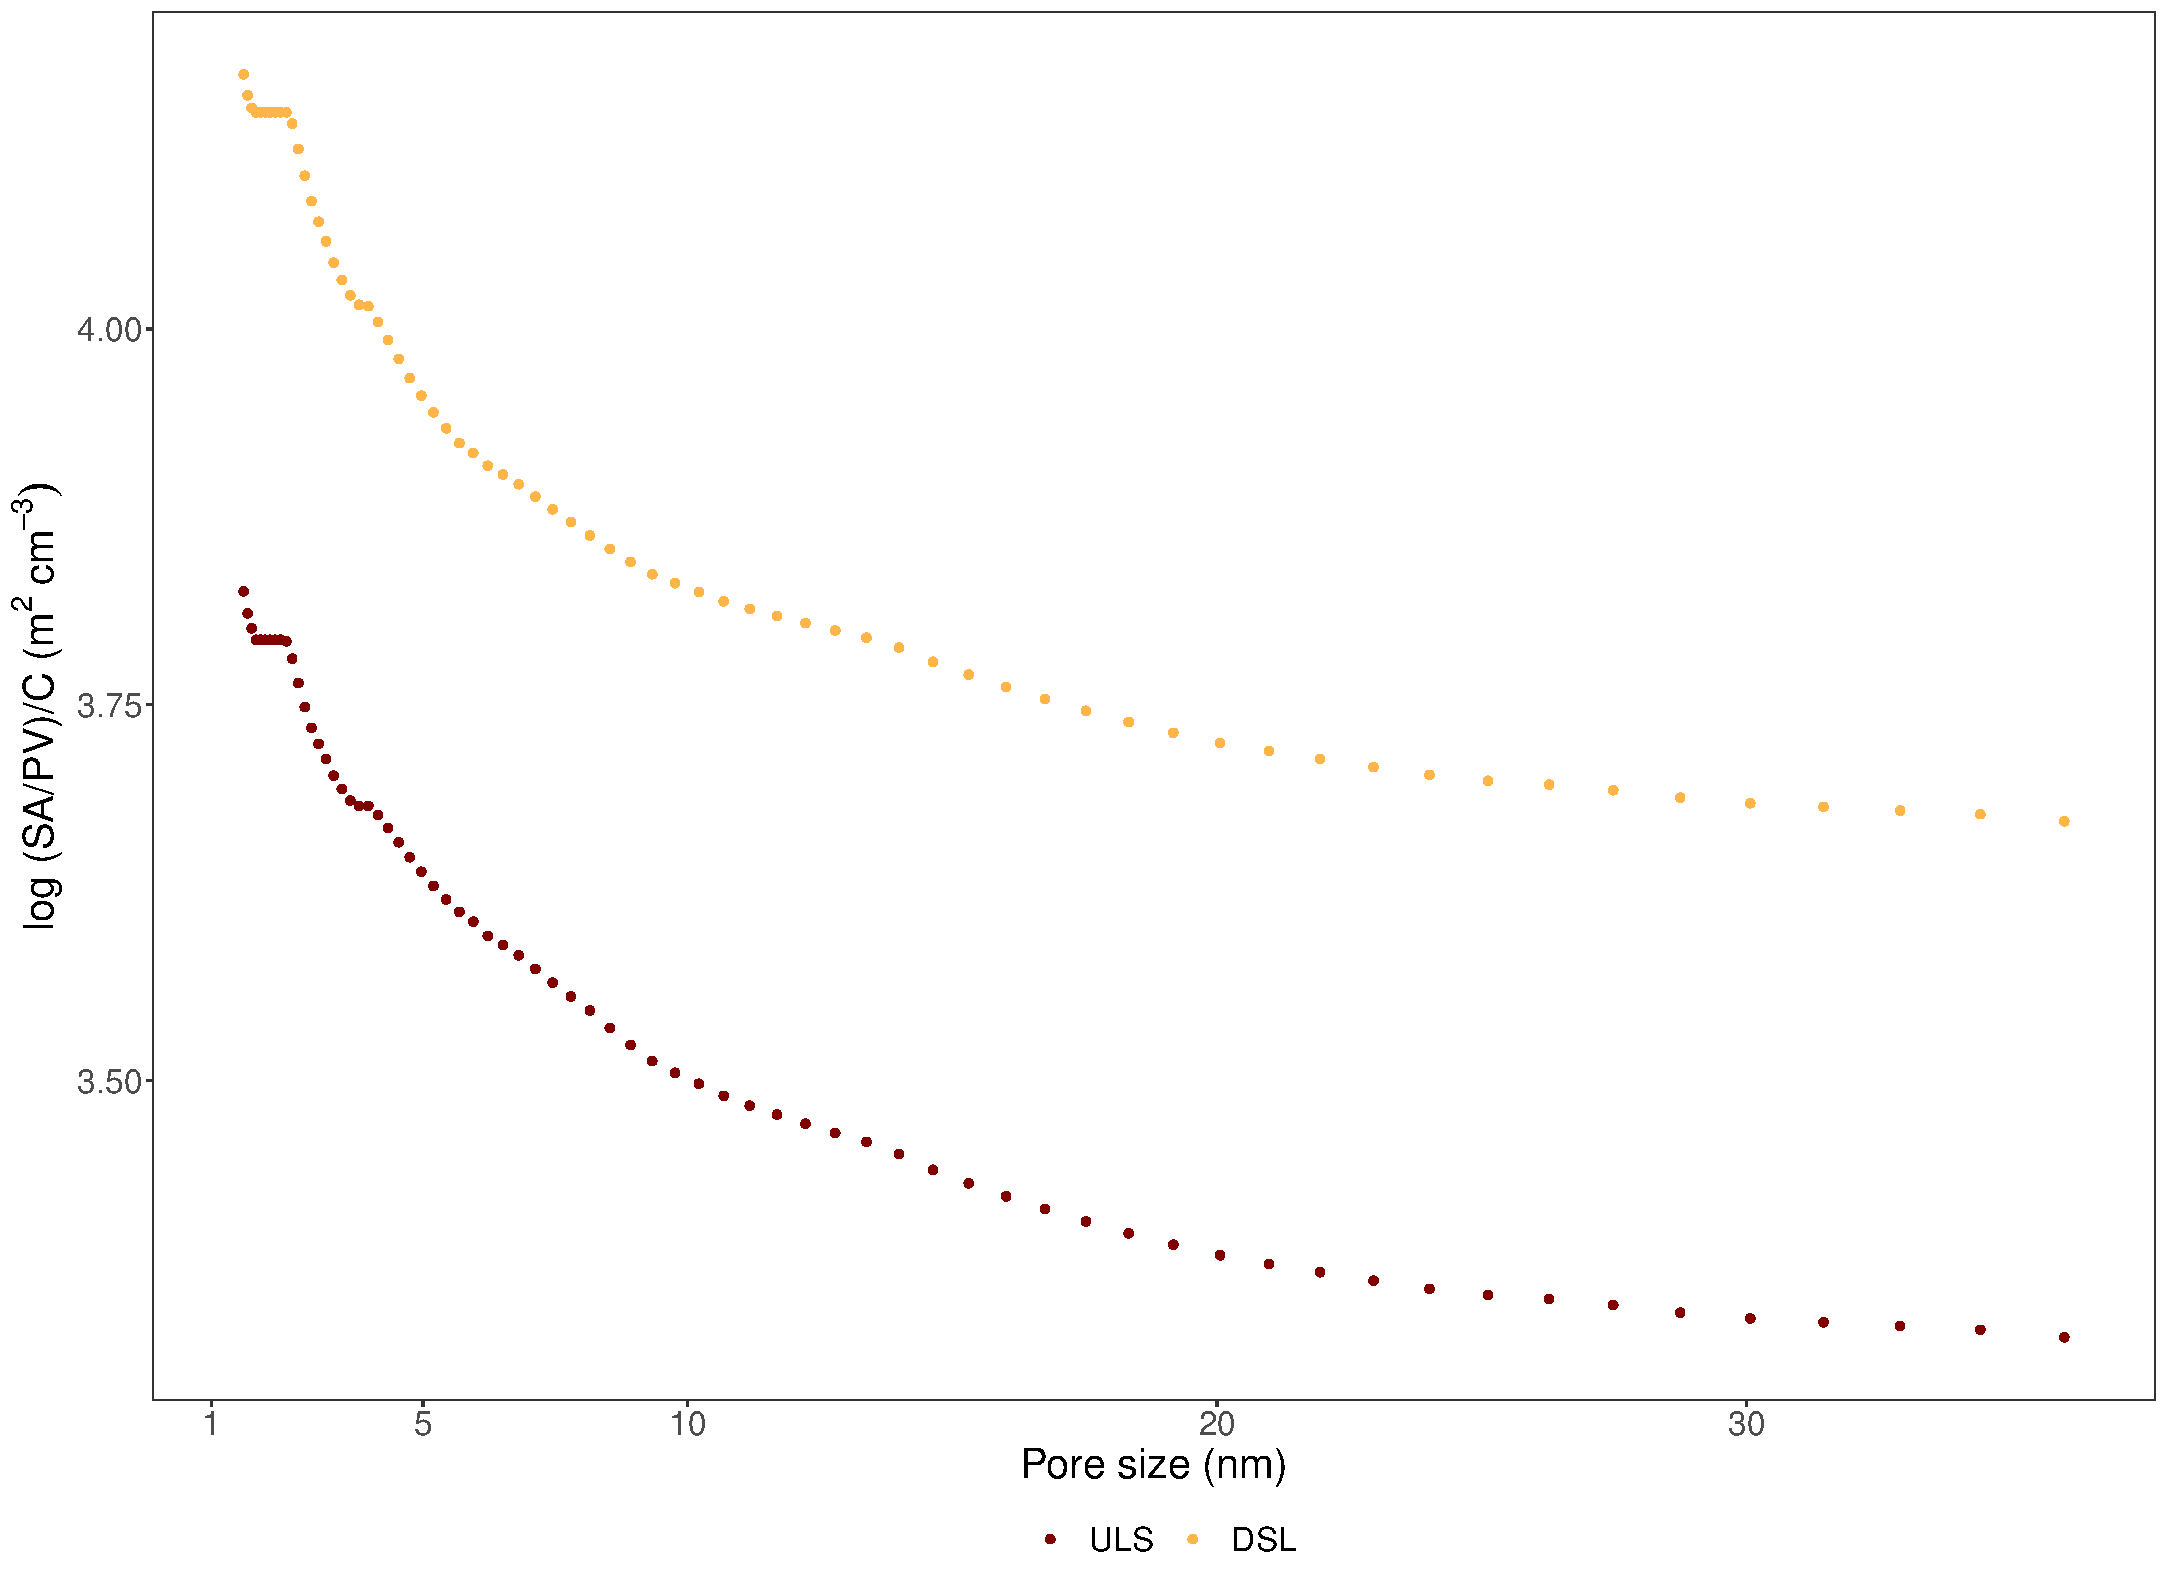
\includegraphics[width=0.45\textwidth]{R/figs/SAPV_C_large.pdf}
}
\caption{Cumulative pore size distribution for pores $>$ 1.5 nm using DFT theory. (a) Surface area, (b) pore volume, (c) SA/PV ratio for pores $>$1.5 nm normalized to carbon content (g C g BC\textsuperscript{-1}). (d) A lower SA/PV/C ratio indicates a higher degree of C in the pore wall matrix.}
\label{fig:PZD_large}
\end{figure}


\citep{yin2022insights,du2014adsorption} effects of salinity on sorption, states sorption increases with increasing salinity because the solubility of PFAS declines when the solution increases in ionic strength, making more PFCs separated from bulk solution onto adsorbents, which is called salting-out effect . 

\begin{figure}
    \centering
        \begin{subfigure}[]{\linewidth}
            \centering
            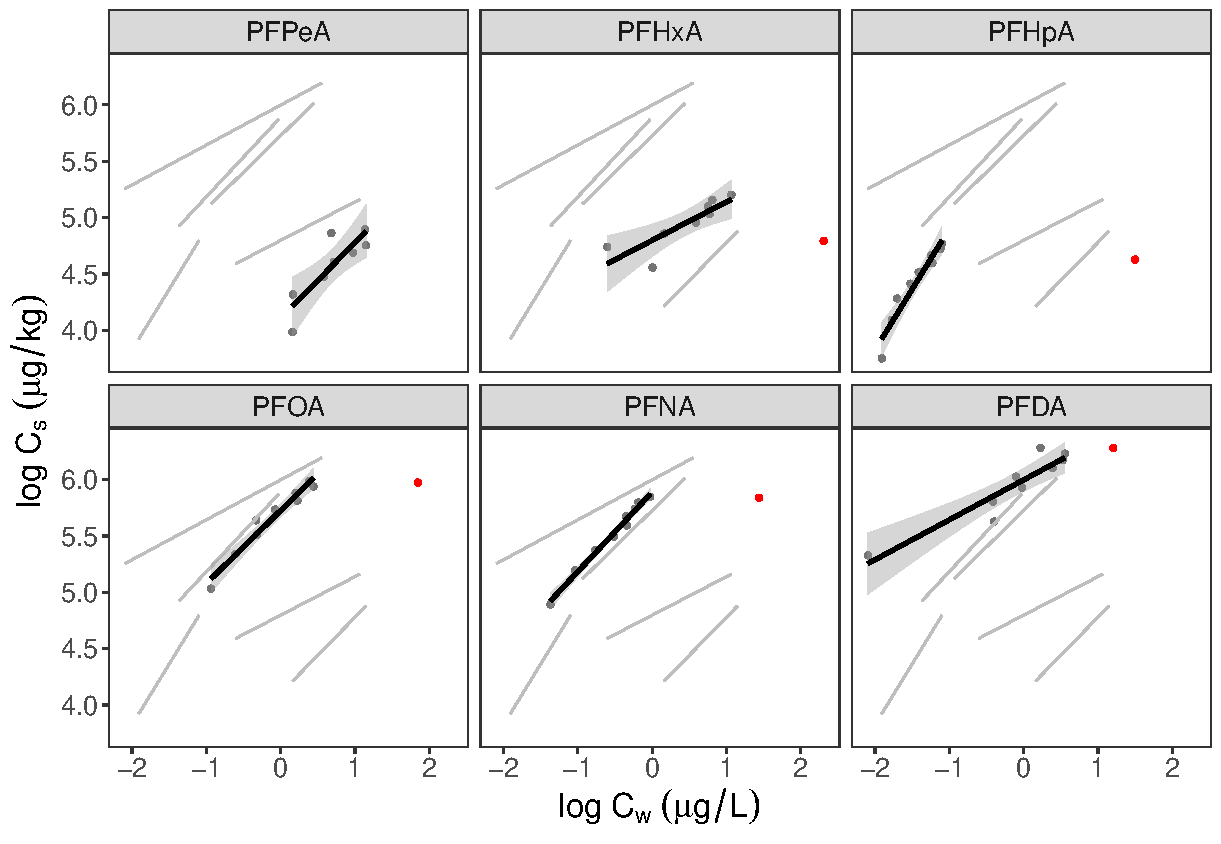
\includegraphics[width=0.6\textwidth]{R/figs/ULS_facet_isotherm.pdf}
            \subcaption{ULS isotherms}
            \label{fig:ULS_isotherm}
        \end{subfigure}
        \begin{subfigure}[]{\linewidth}
            \centering
            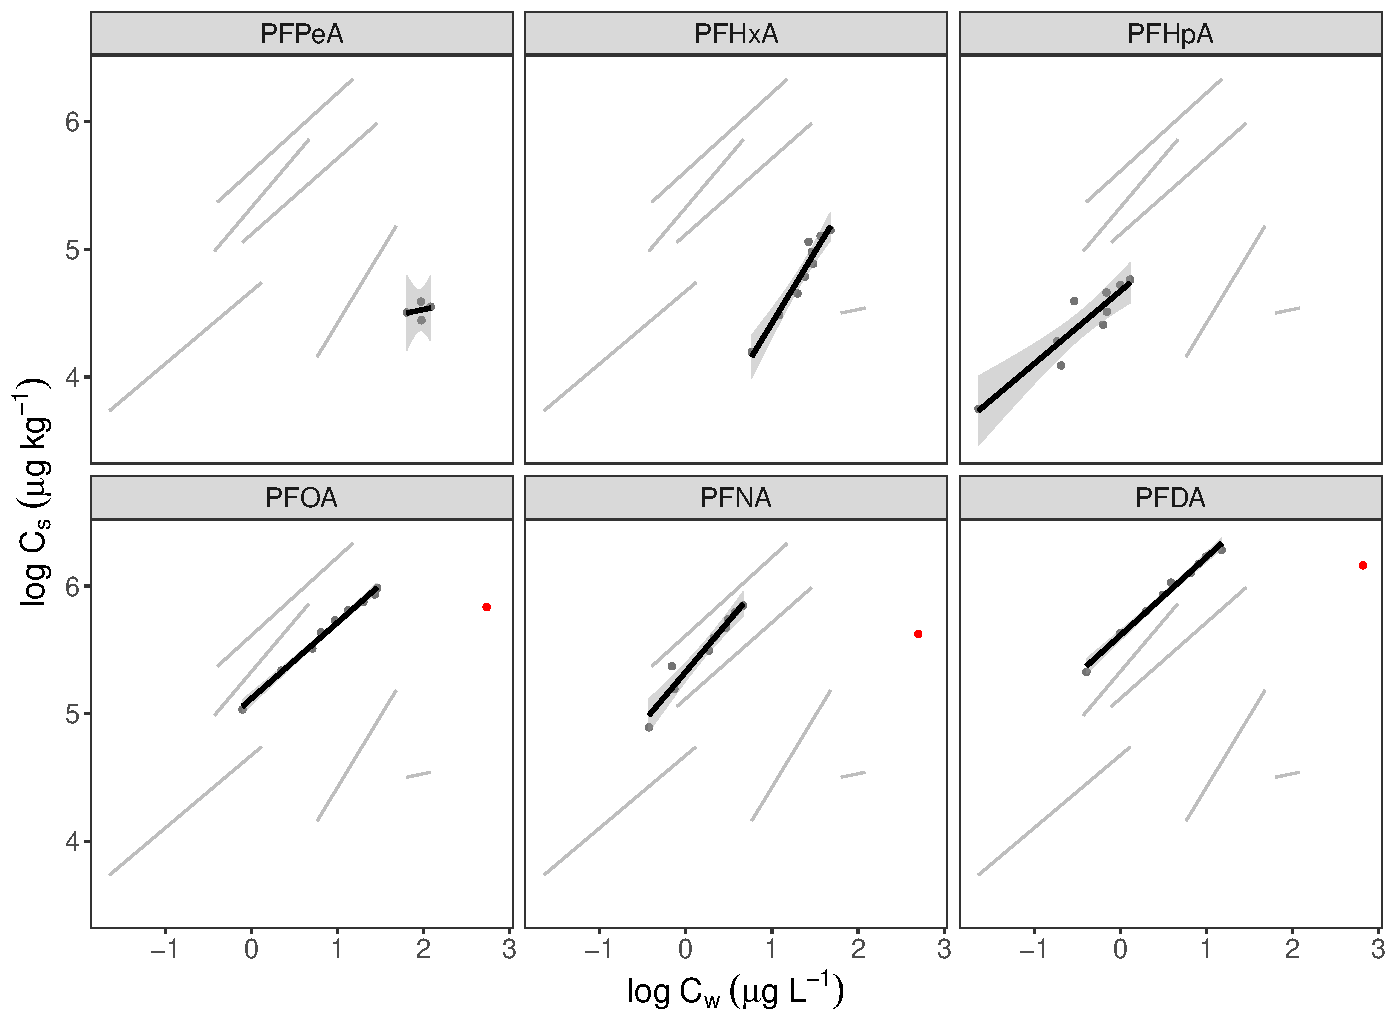
\includegraphics[width=0.6\textwidth]{R/figs/DSL_facet_isotherm.pdf}
            \subcaption{DSL isotherms}
            \label{fig:DSL_isotherm}
        \end{subfigure}   
\end{figure}
\begin{figure}[t]\ContinuedFloat
        \begin{subfigure}[]{\linewidth}
            \centering
            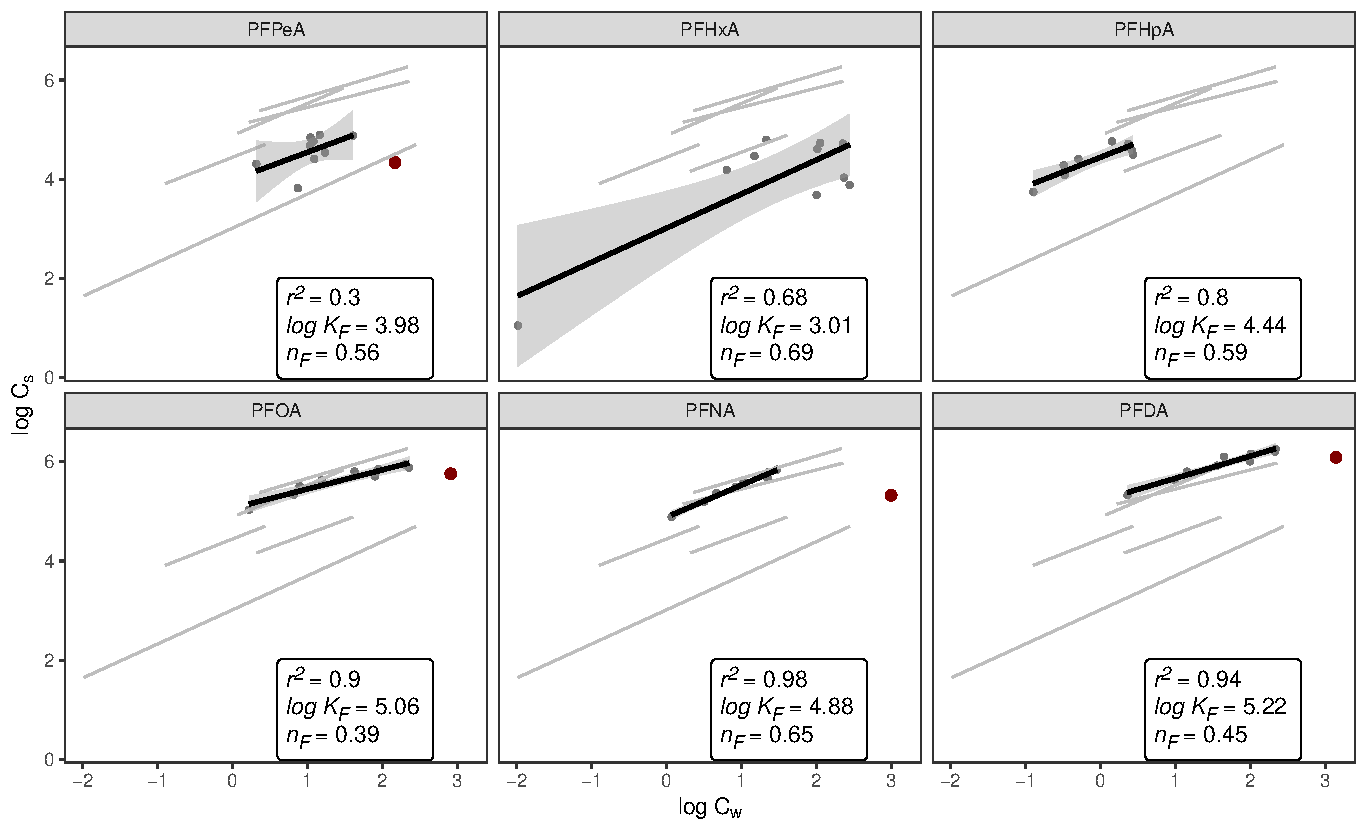
\includegraphics[width=0.6\textwidth]{R/figs/CWC_facet_isotherm.pdf}
            \subcaption{CWC isotherms}
            \label{fig:CWC_isotherm}
        \end{subfigure}
        \caption{Single-compound Freundlich sorption isotherms of PFPeA, PFHxA, PFHpA, PFOA, PFNA and PFDA. Lines are obtained by linear regression. For comparison across chain length, the shaded gray lines are the isotherms from the other compounds.}
        \label{fig:sorption_isotherms_all}
\end{figure}

%Consider removing this table
\begin{table}
\centering
\caption{Competition factor at SC10 (\cref{tab:spikeConcentrations}) for each compound and biochar. Competition factor is defined as K\textsubscript{d,single}/K\textsubscript{d,mix})$\times$100\%.}
\begin{threeparttable}
\label{tab:competition}
\begin{tabular}{lrrr}
\toprule
 & \multicolumn{3}{c}{Competition factor \%} \\ \cmidrule(l){2-4}
 & CWC & ULS & DSL \\ \midrule
PFPeA & 8.2 & \textsuperscript{*} & \textsuperscript{*} \\
PFHxA & \textsuperscript{*} & 2.3 & \textsuperscript{*} \\
PFHpA & \textsuperscript{*} & 0.2 & \textsuperscript{*} \\
PFOA & 15.8 & 3.4 & 4.4 \\
PFNA & 0.9 & 3.4 & 0.7 \\
PFDA & 10.6 & 10.9 & 3.1 \\ \bottomrule
\end{tabular}
\begin{tablenotes}
\item \textsuperscript{*} Amount in filtrate exceeded the amount spiked due to analytical uncertainty.
\end{tablenotes}
\end{threeparttable}
\end{table}

$K_d$ changes the least for PFHxA and PFHpA (2.3 and 0.2 \% respectively) and may be attributed to lower spiked concentrations (330 and 117 \textmu g L\textsuperscript{-1}) for these compounds compared to the rest in \cref{tab:competition}. Competition is most profound for PFOA to CWC followed by PFDA for ULS and CWC (15.8, 10.0 and 10.6 \% respectively), which can be explained by the highest concentrations spiked for these compounds (1 953 and 3 830 \textmu g L\textsuperscript{-1}). It appears that sorption of PFNA is minimally influenced by competition between other compounds despite SC being in the higher range (1 409 \textmu g L\textsuperscript{-1}). $K_d$ for PFPeA is reduced by 8.2\% and is expected based on weaker sorption of short-chain compounds.

\begin{figure}[htb]
    \centering
    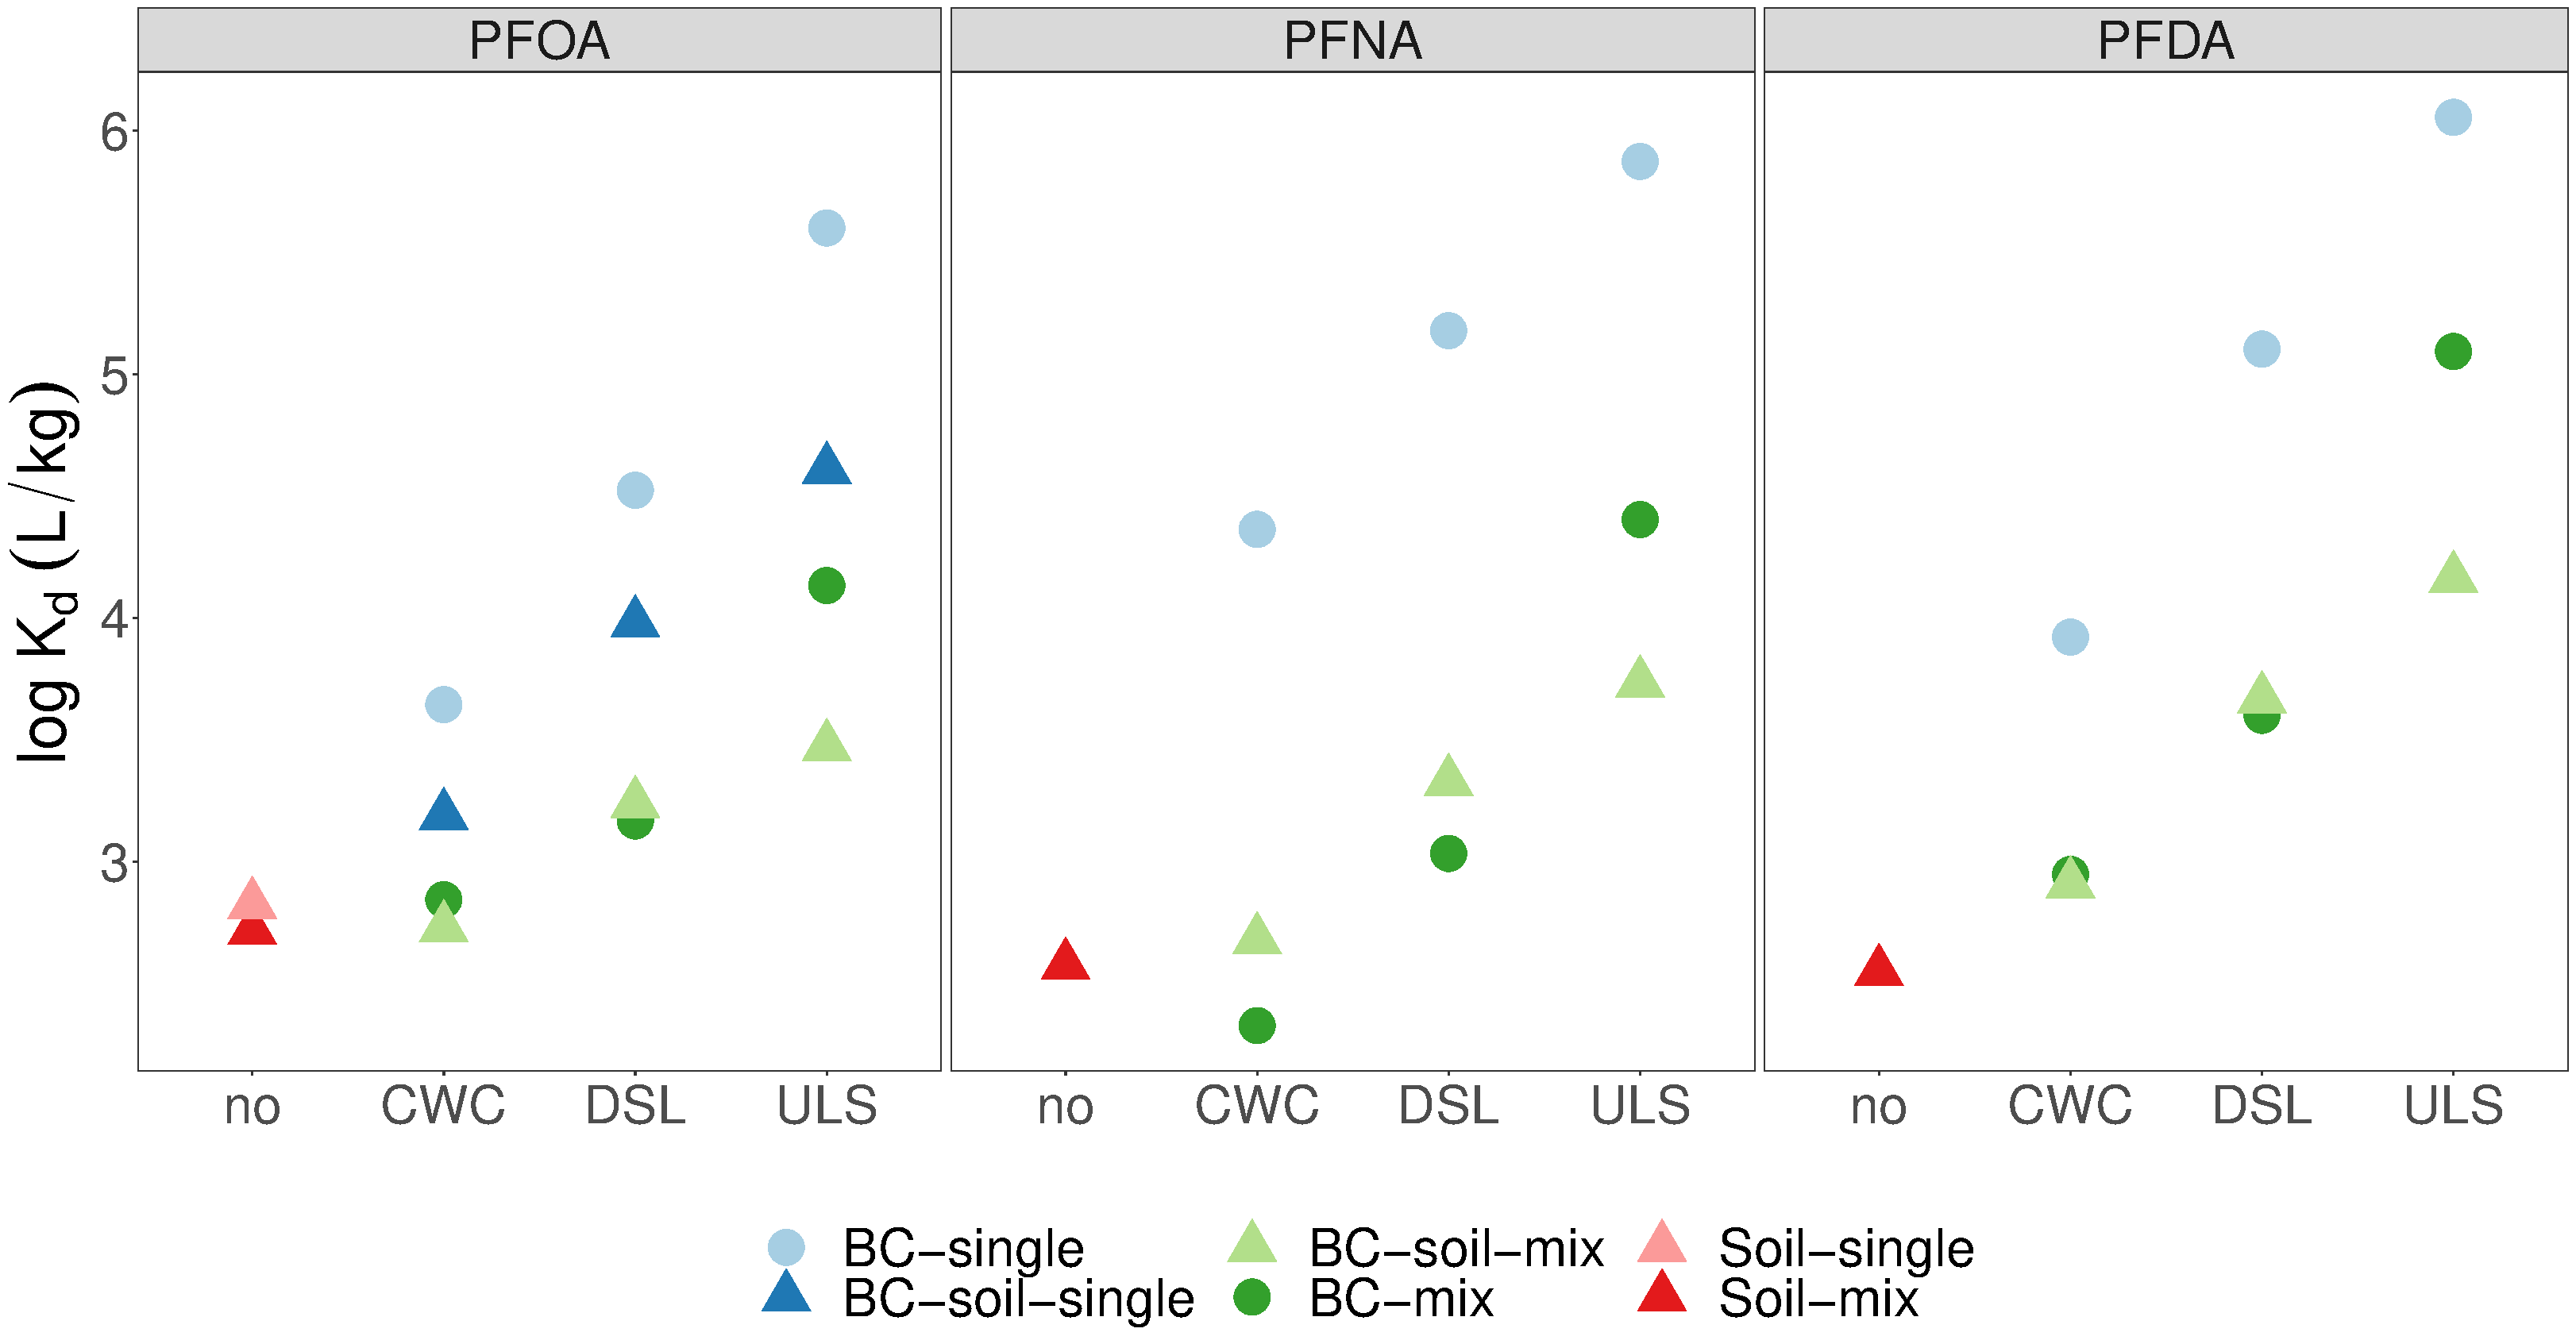
\includegraphics[width=0.8\textwidth]{R/figs/C10.pdf}
    \caption{Sorption attenuation for each TC by soil and/or competing congeners at SC10 (191, 330, 117, 1 953, 1 409, and 3 830 \textmu g L\textsuperscript{-1} for C5-C10, respectively). The error bars represent the standard deviation of $log~K_d$ for the cocktail batch tests performed in triplicate (not included). The single-compound $log~K_d$'s are single points.}
    \label{fig:C10}
\end{figure}
\begin{figure}[htb]
    \centering
    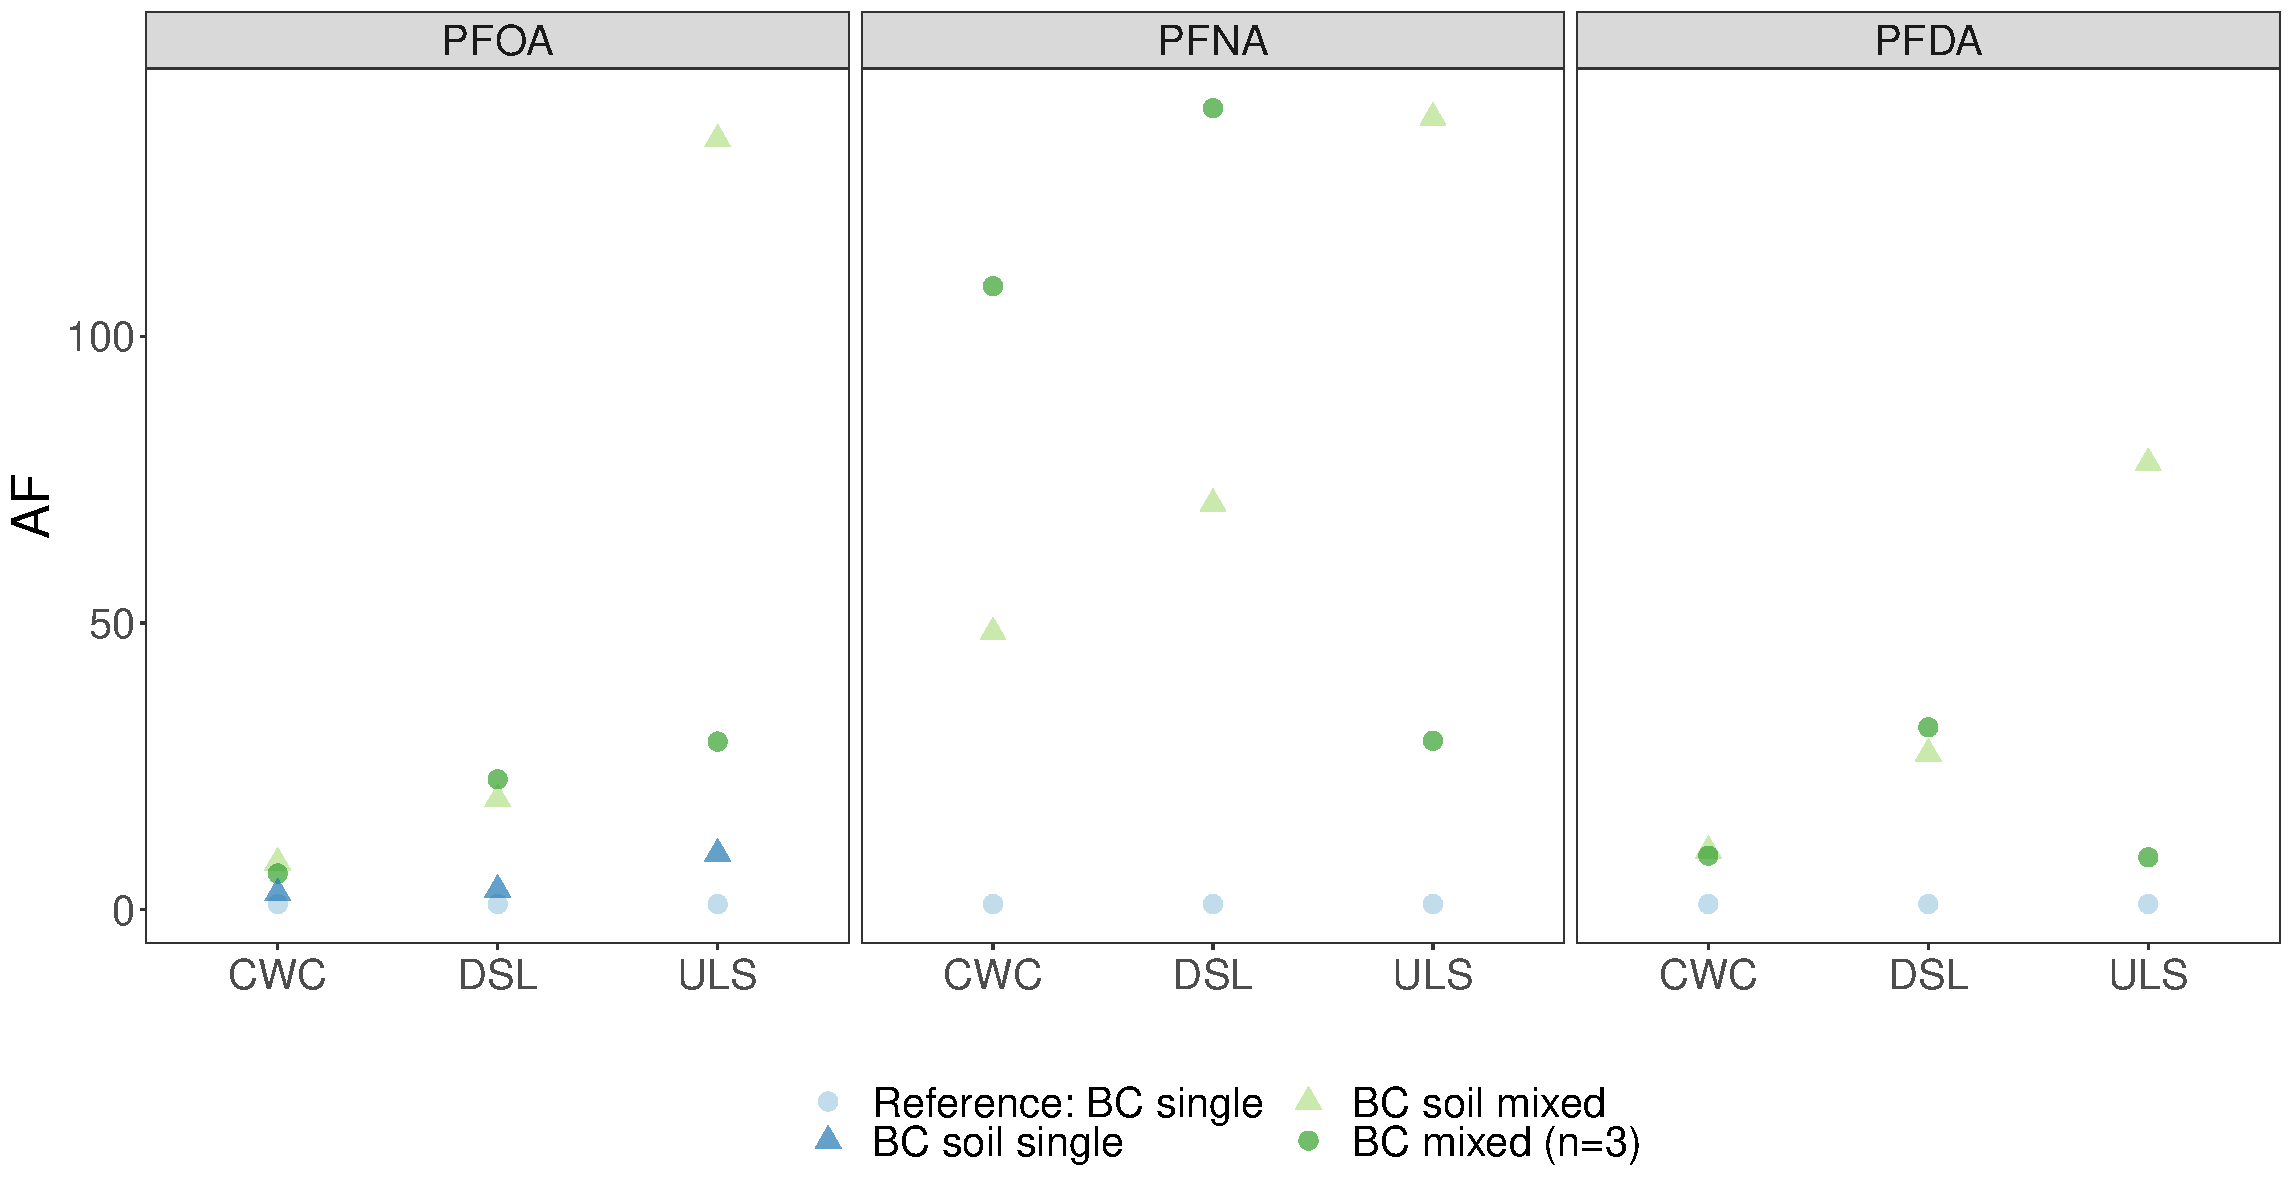
\includegraphics[width=0.8\textwidth]{R/figs/Attenuation_factors_C10_OND.pdf}
    \caption{Attenuation factors at C10 for C8-C10 calculated as \% reduction in $K_d$ from BC single. BC cocktails are spiked with 7.8 mg/L total PFCA and BC soil cocktails with 10.8 mg/L (the difference is due to analytical uncertainty and will be discussed assuming the that the spike concentrations are similar). See \cref{tab:spikeConcentrations} for spike concentrations used for each PFCA in the single-spike and cocktail-spike batch tests.}
    \label{fig:attenuation_factors}
\end{figure}

Attenuation: sorption decreases with time

Make figure showing different sorption mechanisms.\citep{Li2019} is a good place to start. Sorption of PFAS increases with pyrolysis temperature because then porosity and surface area increases.  \textit{in situ} bioremediation vs \textit{ex situ} bioremediation methods, pros and cons of each

The SA/PV better indicates the spatial arrangement of pores, where a low ratio reflects pores of maximum sorption volume

\begin{table}
\centering
\caption{Surface area (SA), pore volume (PV), elemental content (C, O, H, N) and ratios for the biochars produced for the batch tests.}
\adjustbox{max width=\textwidth}{
\label{tab:SAPV}
\begin{tabular}{llrrrrrrlllllll}
\toprule
Biochar & Pyrolysis & \multicolumn{3}{l}{N\textsubscript{2} sorption} & \multicolumn{3}{l}{CO\textsubscript{2} sorption} & \multicolumn{4}{c}{Elemental content} & \multicolumn{3}{c}{Elemental ratio} \\
sorbent & temperature & \multicolumn{3}{l}{(pores \textgreater 1.5 nm)} & \multicolumn{3}{l}{(pores 0.4-1.5 nm)} & & & & & & & \\ \cmidrule(l){3-5} \cmidrule(l){6-8} \cmidrule(l){9-12} \cmidrule(l){13-15} & (\textdegree C) & BET SA  & BJH PV & log SA/PV & DFT SA & DFT PV & log SA/PV & C & O & H & N & O/C & H/C & N/C \\
& & ($\mathrm{m^2~g^{-1}}$) & (cm\textsuperscript{3} g\textsuperscript{-1}) & ($\mathrm{m^2 cm^{-3}}$) & ($\mathrm{m^2~g^{-1}}$) & (cm\textsuperscript{3} g\textsuperscript{-1}) & ($\mathrm{m^2 cm^{-3}}$) & (\%) & (\%) & (\%) & (\%) & & & \\ \midrule
CWC & 700 & 323 & 0.017 & 4.28 & 683 & 0.186 & 3.54 & 91.4 & 5.50 & 1.01 & 0.69 & 0.06 & 0.01 & 0.008       \\
ULS & 700 & 128 & 0.126 & 3.01 & 165 & 0.047 & 3.57 & 29.6 & 57.1 & 1.24 & 1.13 & 1.9  & 0.04 & 0.04        \\
DSL & 700 & 110 & 0.111 & 3.00 & 87  & 0.027 & 3.51 & 13.5 & 61.4 & 1.05 & 0.82 & 4.6  & 0.08 & 0.06       \\ \bottomrule
\end{tabular}}
\end{table}

Based on feedstock type for the three biochars studied in this thesis, carbon content of the biochars follows the expected trend, CWC \textless ULS \textless DSL with 91.4\%, 29.6\% and 13.5\%, respectively 

 Biochar consists of poly-condensed aromatic rings which make the surface \textpi-electron dense, called graphitized surface. Has the ability to bind electron-withdrawing molecules by being \textpi-electron donor. (ring condensation increases with pyrolysis temperature of biochar) PFAS cannot undergo pi interactions because surface also is net negative \citep{Li2019} Literature says that pi pi EDA is an important sorption mechanism between aromatic rings (pi electron donor) and amides (pi electron acceptor). It can be hypothesized that the electron donor/acceptor role can be switched by sorption or PFAS to sludge char which has a high N/C ratio, that could be attributed to amide groups situated in the benzene rings \citep{Li2019}.
 
 Conductivity was 39 \textpm 0.9 \textmu S cm\textsuperscript{-1}. The conductivity of soil-water samples differed the most from the rest of the samples with a mean conductivity of 23 \textpm 0.05 \textmu S cm\textsuperscript{-1} versus a mean of 41 \textpm 0.9 \textmu S cm\textsuperscript{-1} for the biochar-water and biochar-soil-water samples. 
 
 \cite{du2014adsorption} summarizes that the more basic groups the adsorbents have, the more PFAS they adsorb, which is somewhat counter intuitive when considering potential repulsion by the anionic PFCA functional group and the established connection between a degree of condensation (low O/C and H/C ratios). The reason for this is that these groups are typically weak acids that are prone to be protonated at environmentally relevant pH's. 
 
 Influences adsorption ability of environmental contaminants depending on surface morphology, especially hydrophobicity. In terms of PFCAs, biochar is expected to be a better sorbent at low pH due to limitation of electrostatic repulsion of biochar functional groups and the polar head of the perfluoroalkyl carboxylate. 
 
 , and salting-out. The latter mechanism occurs only at high enough salt concentration and is not applicable for the present study. 
 
 increase in zeta potential
 
 The presence of electrolytes creates an EDL that changes the adsorption surface of biochar \citep{du2014adsorption}.
 
 Ca\textsuperscript{2+} and Mg\textsuperscript{2+} in the EDL can function as bridges between the negatively charged functional groups of PFAS and surface negative charges.
 
Rather than the soil contributing additional sorption capacity, soil attenuates the effect of the biochar sorbents by pore clogging and competitive sorption to pore walls than enhancing sorption by the presence of additional sorbent substrate because DOC keeps some PFCAs still in solution \citep{Li2019}.
 
\crefrange{subfig:C10}{subfig:AF}, the effect of soil on $K_d$ is visualized by the difference in the blue circles and triangles. $log~K_d$ drops by 65\%, 71\%, and 90\% for CWC, DSL and ULS, respectively. Attenuation is lowest for BC soil single, 12-18 \% of maximum sorption, but note that only PFOA was spiked for this batch test feedstock.
  
$n_F$ is a dimensionless empirical parameter that represents sorption linearity.

The batch tests were spiked at 10 concentrations over four orders of magnitude where the lowest concentration was aimed at being close to the instrumental LOQ. 

From other studies, $K_F$ increases and $n_F$ decreases with decreasing O/C, H/C, and N/C ratios \citep{Cornelissen2005}. However, this study $K_F$ decreases with decreasing O/C, H/C, and N/C ratios, and no clear trend is seen for $n_F$. Meanwhile, it does seem like the nonlinearity coefficients for CWC are more stable with increasing chain lengths than ULS and DSL. Additionally, comparing $n_F$ across compound isotherms does not make sense due to different spike concentrations being used for each compound.

Concentration interval for the isotherms is an important predictor of the slope ($n_F$) and intercept ($log~K_F$) derived from the linear regression.  The Freundlich coefficient of non-linearity ($n_F$), is a measure of sorption capacity within the concentration range acheived for the sorption isotherms. A lower $n_F$ indicates that sorption sites are starting to be saturated and the biochar is closer to its maximum sorption capacity.  For PFPeA- and PFHxA-CWC, it appears that CWC sorption sites have been saturated since most points center around the same area, which means that CWC reaches sorption maximum at $~$4 000 $\mu g~kg^{-1}$. However, four points are insufficient to conclude that CWC has the lowest affinity and capacity to sorb short-chain PFCAs. 

Sorption non-linearity ($n<1$) occurs due to the complex composition of sediment/biochar with both positive and negative charges contributing to either attraction or repulsion, as well as hydrophobic surfaces, and indicates successive saturation of these adsorption sites \citep{yin2022insights}. 

\subsection{Sorption processes in natural systems}\label{sec:natural}
Only $~7\%$ of the numerous minerals in global soils have surfaces that are net positively charged at ambient pH, most importantly Fe-oxides and Al-oxides. 

Efficiency of biochar sorbents in complex systems must be evaluated in order to say something about their suitability for the intended uses because simultaneous presence of a diverse suite of organic contaminants with soil and sediment generally change sorption mechanisms and weakens sorption strength \citep{zhou2010sorption}.

Applied to real-world conditions, this means that soil amended with BC is more effective in removing PFCAs at low concentrations than highly contaminated soil with a mixture of compounds and high total water concentration of PFCAs.

Interaction of fouling and time: given enough time, fouling is less \citep{Werner2006}. Functional groups are typically located on the external part of biochar which can hydrogen bond with surface groups on humus preventing hydrophobic contaminants from entering the pores. Coating by humic material in high TOC soil, pore blocking \citep{Hale2011}.
Sorption generally decreases with increasing pH due to electrostatic repulsion between negatively charged surfaces and negatively charged PFAS \citep{du2014adsorption}. Cation bridging effect in high pH by presence of earth alkalis, increases sorption even at high pH \citep{du2014adsorption}. Relevant for adsorption to sediment, black carbon. "Competition: inorganic anions can compete with anionic PFCs for adsorption sites, resulting in a decrease of PFCs sorption on adsorbents" \citep{du2014adsorption}. 
\citep{Sormo2021}: OM can weaken sorption to biochar due to pore blocking. One might think that soil high in organic matter will be strengthen sorption when amending the soil with biochar, however, this turns out to be the opposite. Refer to figure from \citep{Cornelissen2005}. Organic matter competes as sorption sites for PFAS but the sorption strength is weaker so desorption will occur more easily than once sorbed to biochar. 

As described in \cref{sec:S-BC}, the batch tests with soil and soil-CWC Aggregation of humic substances as brown fluff was observed upon addition of 1 M acetic acid to pH 3 pre-SPE for the most colored filtrated samples \cref{subfig:precip}, indicative of humic acids. At low pH, humic acids protonate, which leads to less electrostatic repulsion between acid functional groups within the DOC molecules so that they aggregate and precipitate from solution. During SPE, PFCAs that had sorbed to the DOC would be extracted and contribute to an overestimation of . 

\begin{figure}[tbh]
\subfloat[\label{subfig:filtrate}]{%
  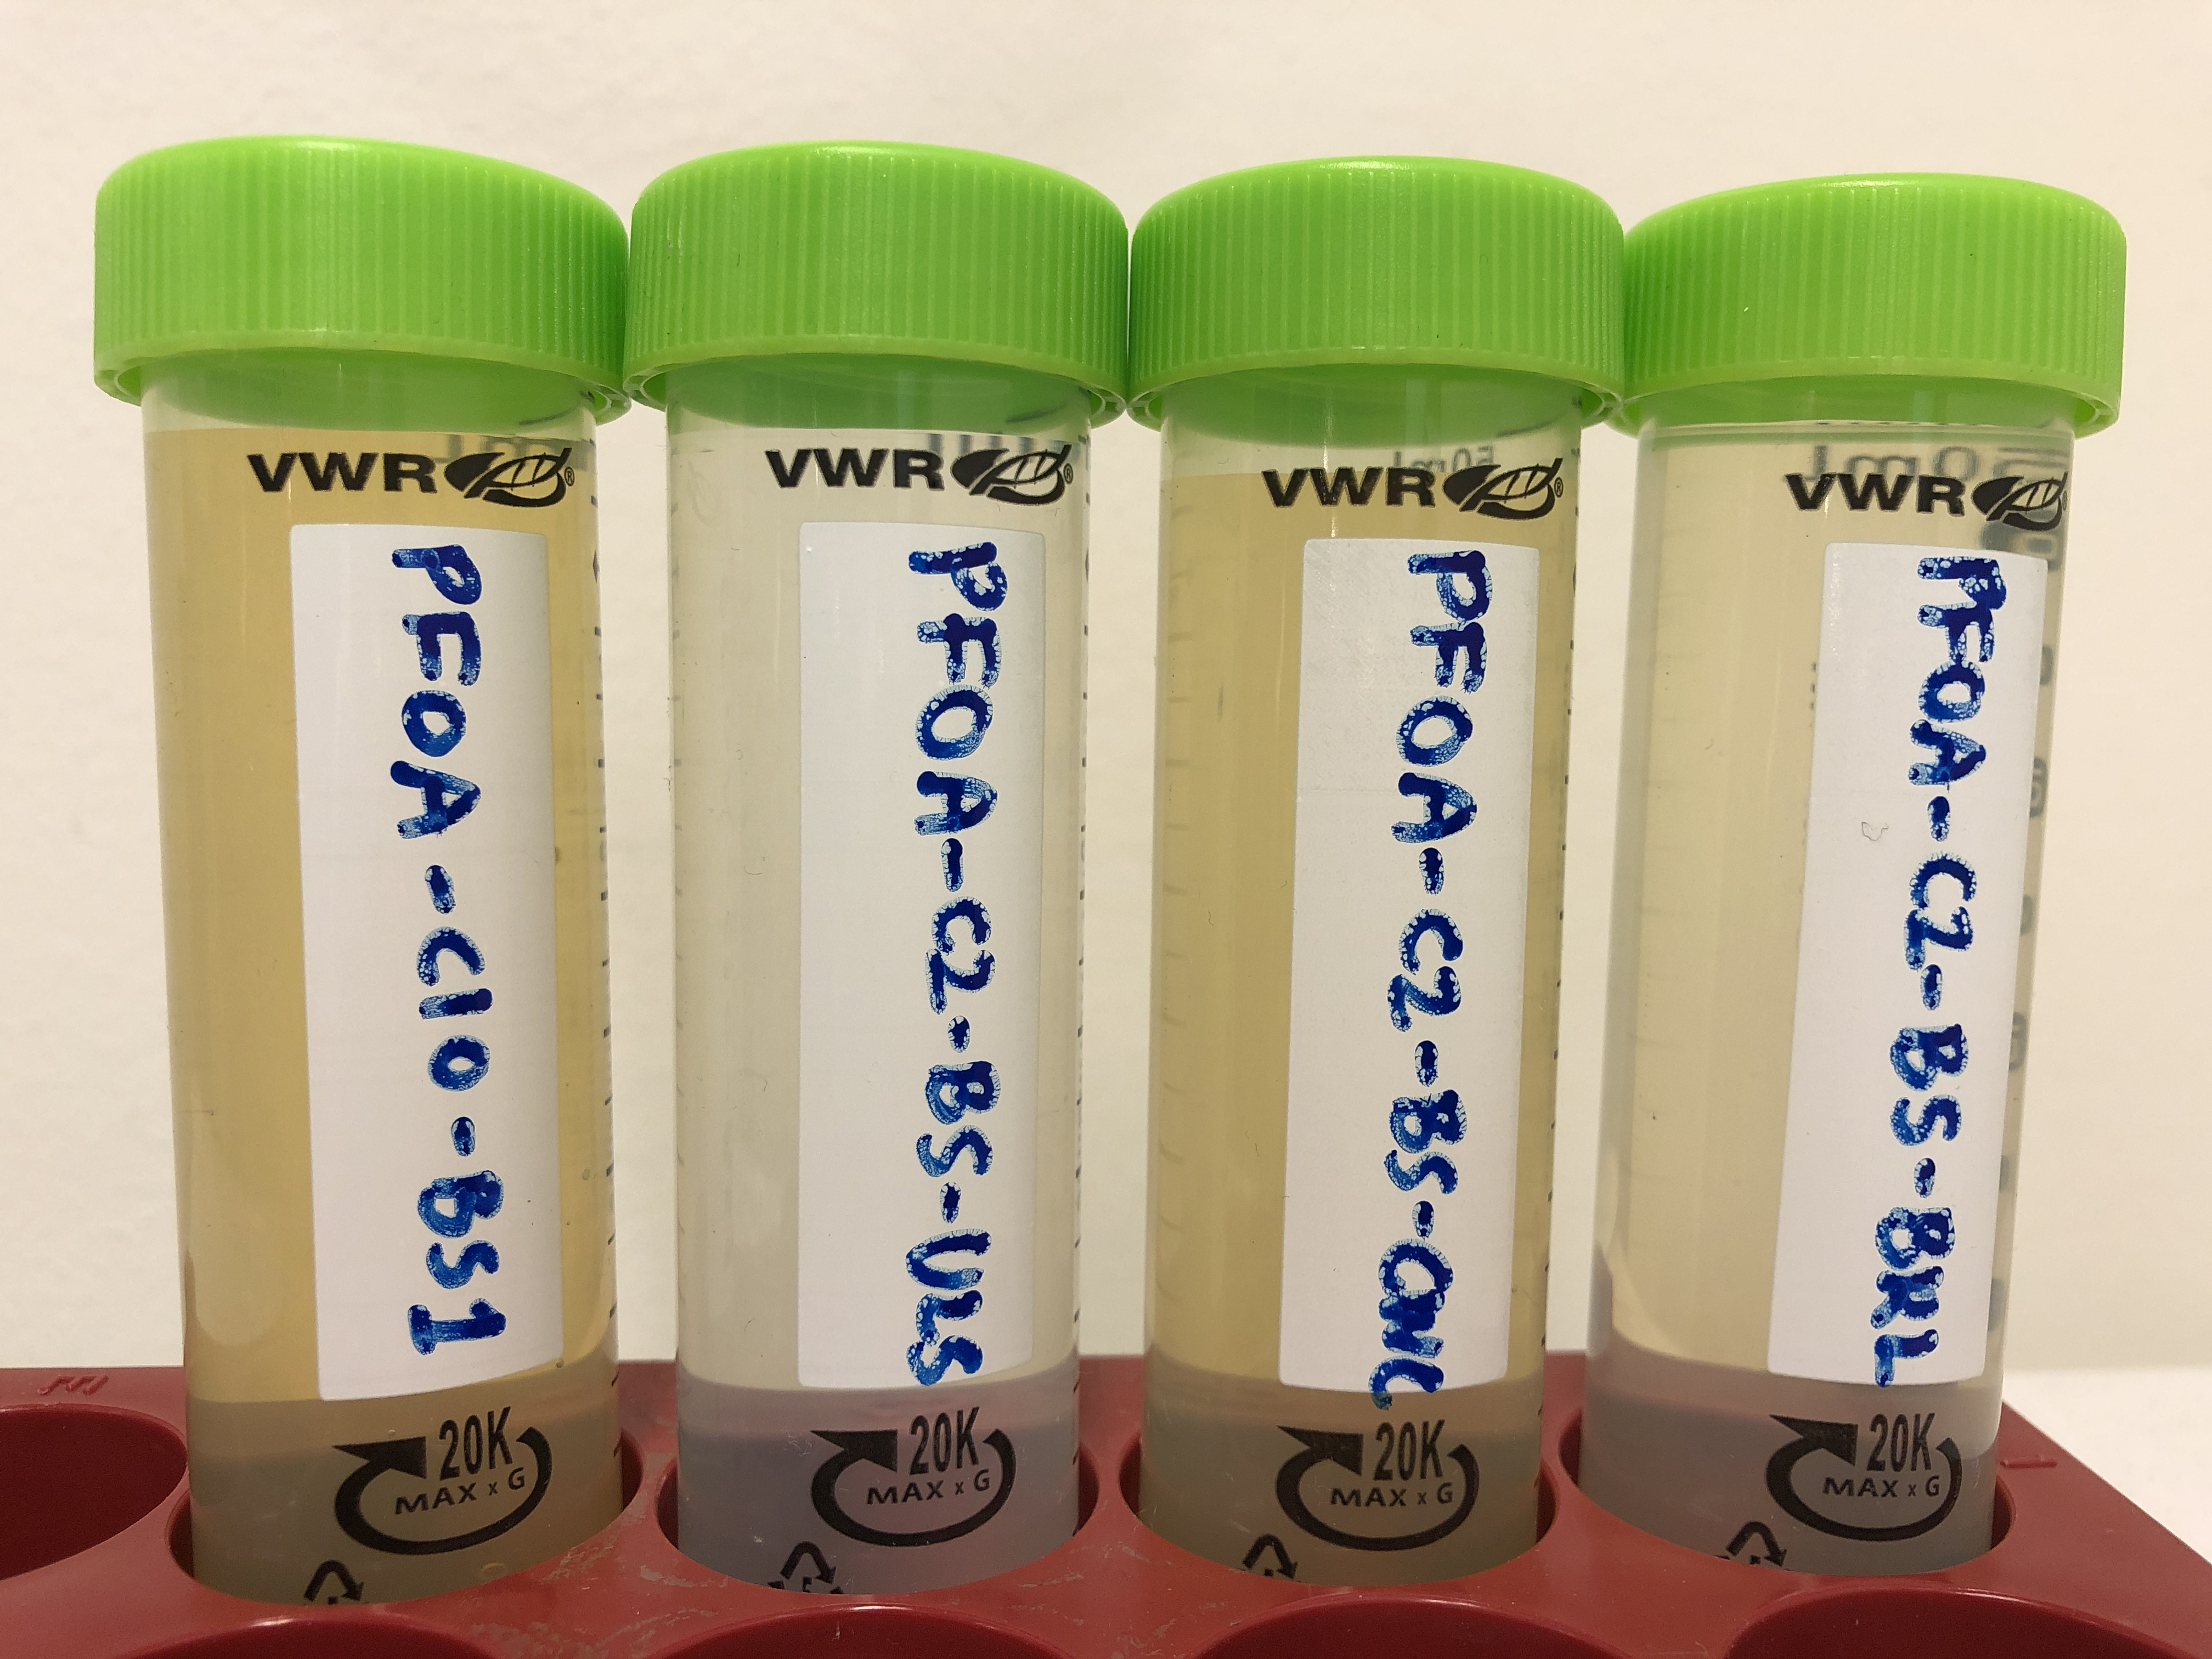
\includegraphics[width=0.45\textwidth]{Bilder/Samples/Filtrate_DOC.JPG}
}
\hfill
\subfloat[\label{subfig:precip}]{%
  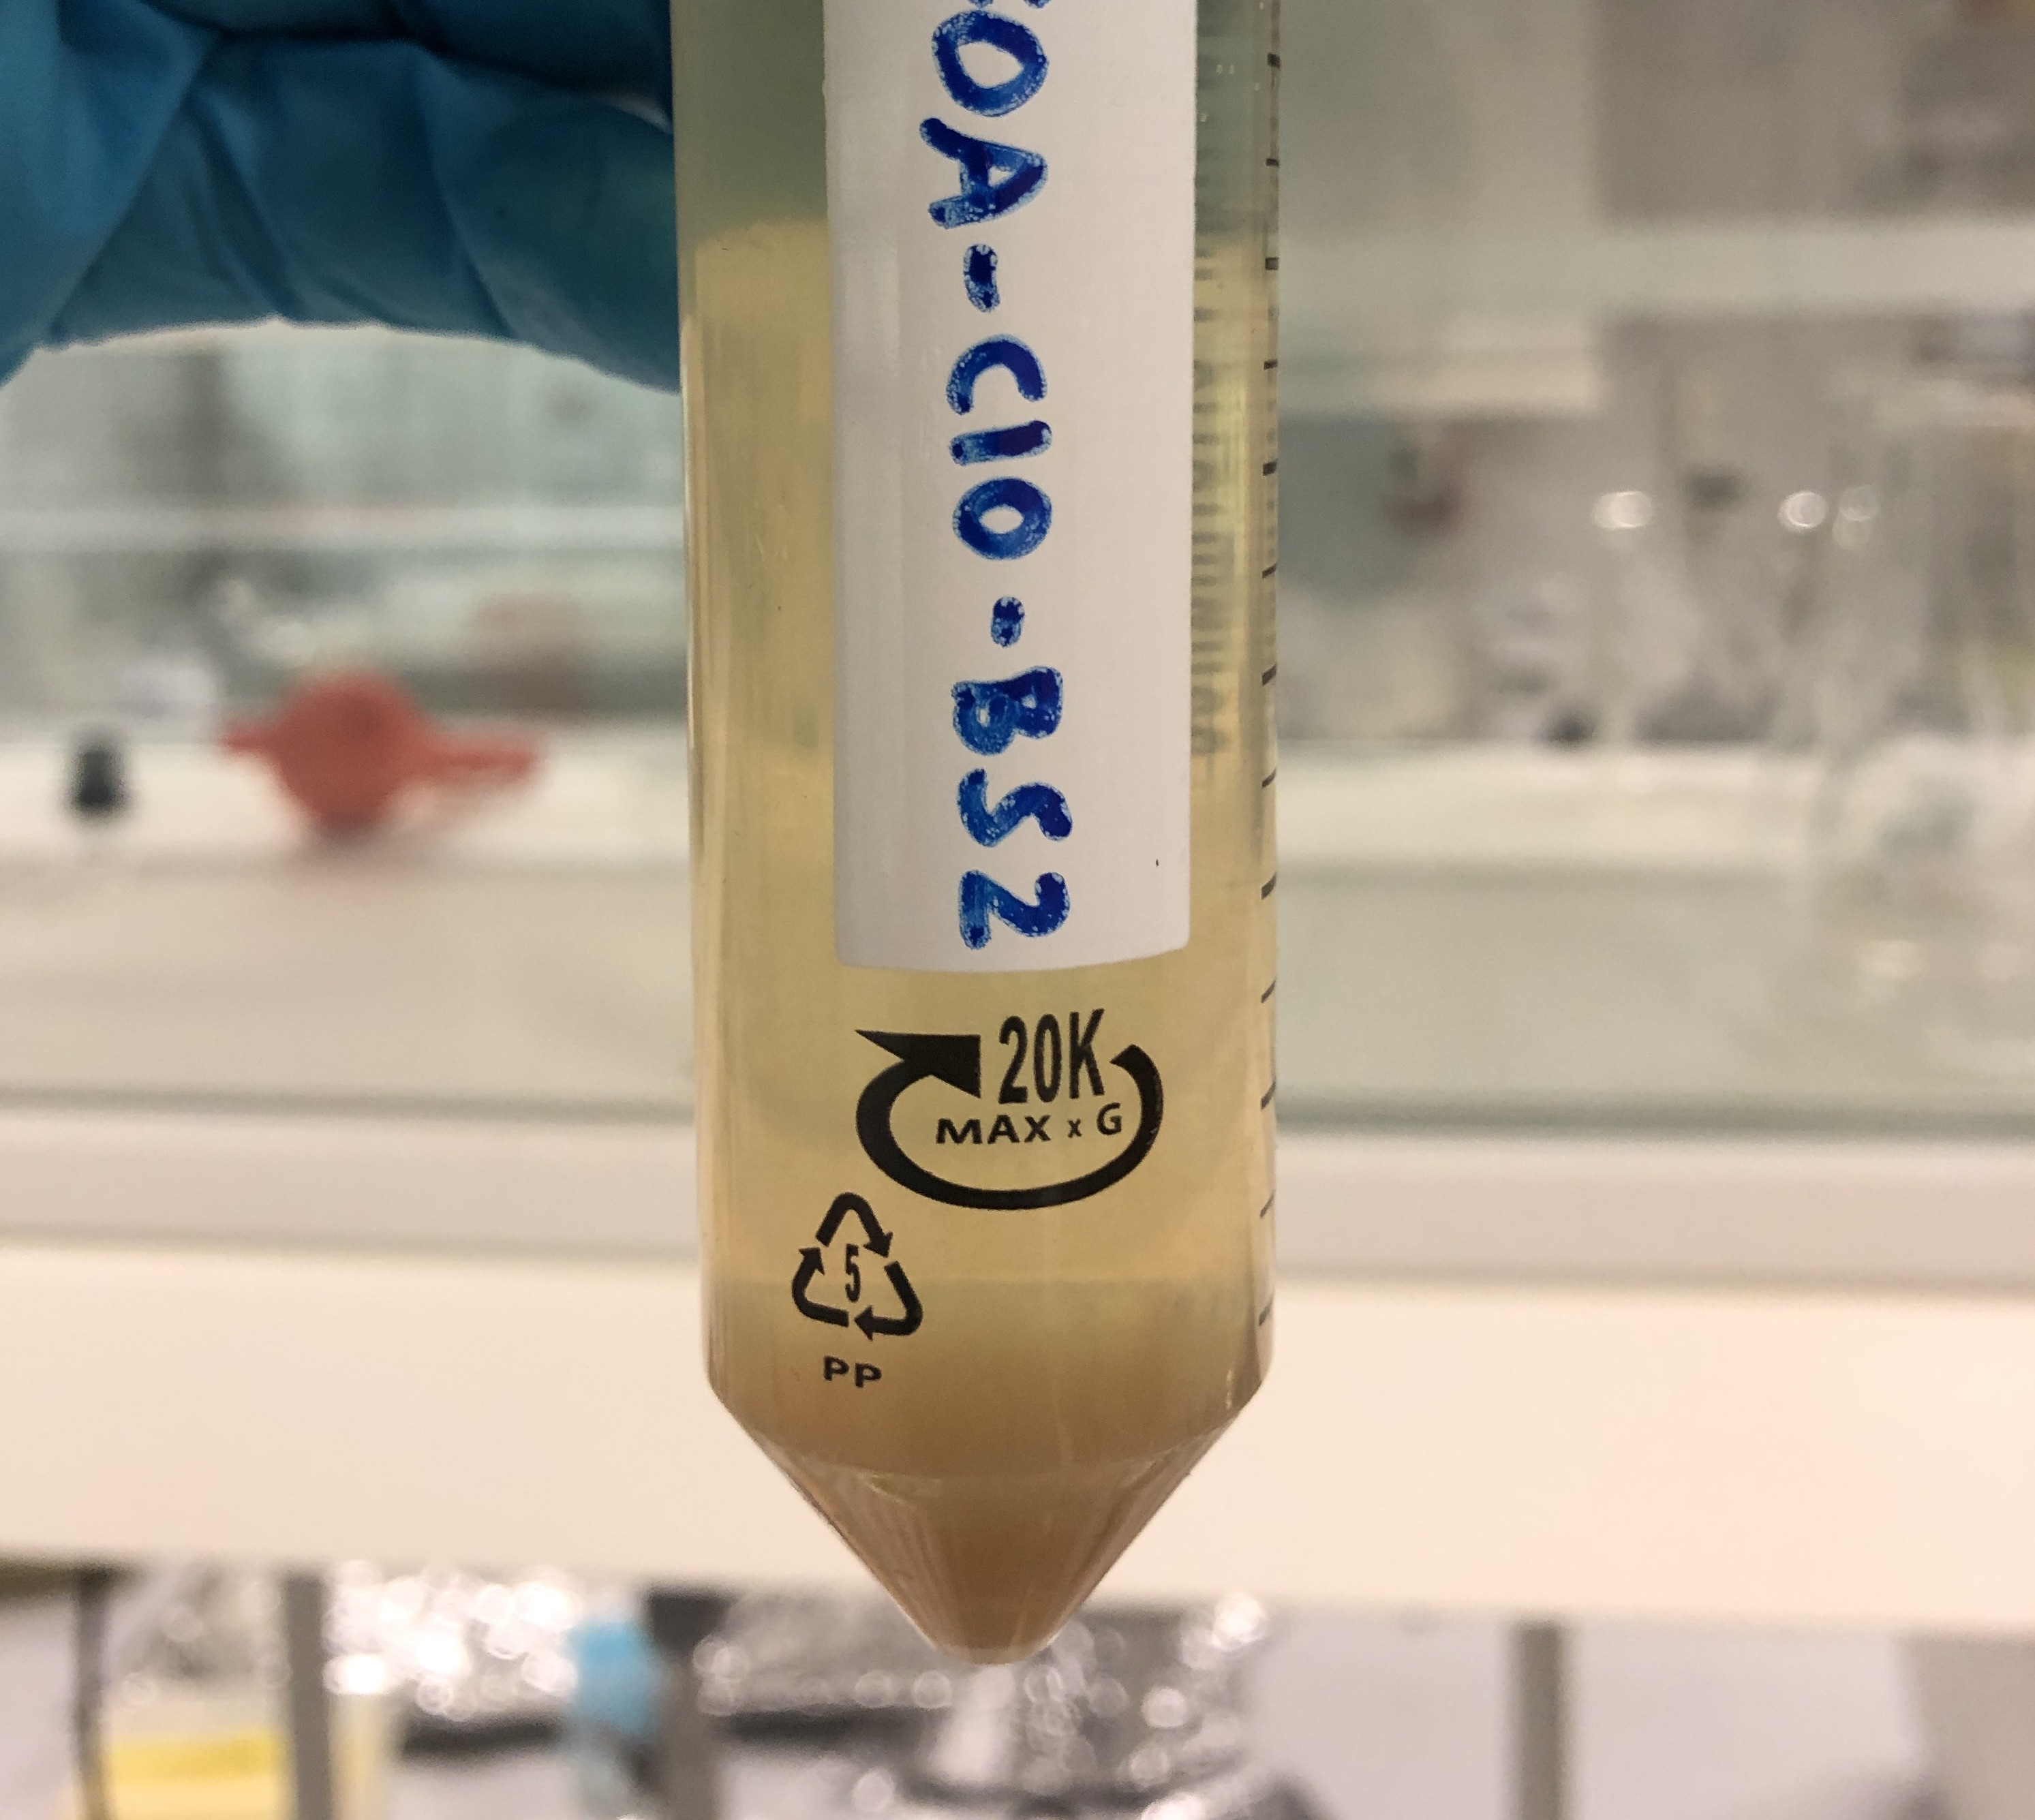
\includegraphics[width=0.38\textwidth]{Bilder/Samples/Precipitation.JPG}
}
\caption{(a) Color of filtrate for each biochar batch test. From left to right: soil only, soil+ULS, soil+CWC, and soil+DSL (BRL = DSL). (b) Precipitation observed when filtered soil samples were adjusted to pH 3 with 1 M acetic acid.}
\label{fig:DOC_tubes}
\end{figure}

pH (although liming raises pH which is not good for sorption, addition of Ca\textsuperscript{2+} creates divalent bridging effect and complexation of PFAS molecules that enhance sorption. 

\subsubsection{Field conditions representativeness}

Equilibrium conditions vs laboratory batch tests
BC dose

Are the results representative of what goes on in real life? Sorption by shaking for 14 days represent an assumed equilibrium between PFCAs in the water and soil phase. A comparable situation in the field would be washing of the soil with large amounts of water such as during heavy rainfall. This will only be the case during occasional stormwater events and thus the results from this research could benefit from being supplemented with results from leaching tests using biochar mixed with soil. However, the relationship:

\begin{align}
    \frac{k_1}{k_2}
\end{align}

where \(k_1\) is the PFCA sorption (adsorption and absorption) rate and \(k_2\) is the PFCA desorption rate, where \(k_1>>k_2\), which indicates that sorption is many times higher, and in an equilibrium situation, sorption and desorption will be at steady state \citep{Cornelissen2005}. 

Leaching of heavy metals results at PT 700 C
    As, Cd, Co, Zn, Pb for all chars Below EBC limits, Cr and Ni between lower and upper limit
    EBC = European Biochar Certificate
    Cu above EBC limits for ULS and DSL
    Enrichment factors heavy metals (?)
Will pyrolysis remove PFAS? Draw parallel to pyrolysis of PTFE (Teflon) that occurs when pan is heated to above 300 \textdegree C, can get polymer fume fever from toxic fumes (carbonyl fluoride and trifluoroacetyl fluoride)

If CWC was activated, it would likely become a much better sorbent because most of the smallest pore spaces previous inaccessible to PFAS would be expanded, giving CWC the lowest log SA/PV/C ratio.

High operating energy and cost different technologies \citep{Alhashimi2017}
Energy demand pyrolysis 
Energy production occurs from pyrolysis reactions through the gaseous and liquid fuels that are created as co-products, however, bio-oil from pyrolysis of sewage sludge is likely unsuitable as energy source

"compared to the highly exothermic incineration, most of the pyrolytic reactions are endothermic consuming energy of around 100 kJ kg\textsuperscript{-1}
 
The charcoal vision \citep{Laird2008}: "A win-win-win scenario for simultaneously producing bio-energy, permanently sequestering carbon, while improving soil and water quality".  

Green Deal is another initiative by the European Commission that aims to make the European Union climate neutral by 2050. Fresh air, clean water, healthy soil and biodiversity is a central part of the main initiative aims that are to transition Europe into a circular economy.

Since the diameter of the centrifuge tube (30 mm) was larger than that of a volumetric flask and biochar was added prior to the dilution process, the final concentration of the sorbent-sorbate mixture may have a heightened inaccuracy. However, the volume of which 0.1 g biochar occupies can be considered insignificant due to the high absorptive capacity of biochar and small mass used. 

The three pipettes were: 1) 2-10 mL, 2) 200-1000 \textmu L, and 3) 5-50 \textmu L.

\subsubsection{Batch tests}
Vel, du kan jo prøve å legge sammen alle de feilene. Det finnes jo forskjellige typer feilkilder i et stort forsøksoppsett. Det man ofte ser er at det er en eller to feil som er så store at de overskygger de andre. Da er det ikke noen vits å ta med alle de små. Feilen som ofte er størst er reproduserbarhet av metoden. Altså forskjellen mellom for eksempel prøver laget i triplikater. Det du kan gjøre i oppgaven din er jo å kort diskutere feilkildene du har og identifisere de største og viktigste.

\citep{Lath2019labsorb}: 
Syringe filters: sorption of PFOA to centrifuge tubes and filter membranes. Sorption onto syringe surface: negligible due to short residence time (\textless 10 s). . No improvement in recovery was seen when conditioning the syringe filters with phosphate solution or methanol.

Test tubes: Greater recoveries from glass tubes than plastic, PP poorest recovery (55-68 \% recovery)... Contact time of PFAS residing in tubes for longer than 7 days should not be of significance, as \citep{Lath2019labsorb} propose that sorption and saturation of tube walls occur within hours. 74-81 \% recovery for PP when testing dependence on pH and ionic strength. Slight pH dependence, higher recovery at higher pH due to repulsion of negatively charged functional groups (PP has negative surface charge above pH 3.5-4. Bridging effect will be observed at higher pH's between cations like Ca2+, but is still considered negligible compared to the losses due to the physicochemical properties of the materials themselves. In general PP and plastics consists of mainly carbon hydrogen chains and are more hydrophobic than glassware. 
The polypropylene (PP) tubes used for the batch tests did not have the greatest recovery among different materials tested. 

SPE protocol, many steps, many PP test tubes transfers, saturated PFAS-solutions, internal standard (dilutions had to disregard IS because too low concentration). 

Calibration curves and matrix effect, 3-point curve
LC-MS/MS

Manual review of peak integrations
decisions to remove C1 at low signal
where observed similar peak integrations across concentrations, suspected saturation of detector, dilution of these samples

Due to the novel research on sewage sludge biochars as sorbents for PFAS in this thesis, literature partitioning coefficients for PFCAs to other sewage sludge biochars are non-existent to the author's knowledge.

London dispersion forces (induced dipole-induced dipole attraction), the weakest intermolecular force, make the bonding so strong, not Van der Waals forces,  separation distance, condensed aromatic carbon surfaces \citep{Cornelissen2005}

%\citep{Ahmad2014}: table 3 lists sorption mechanisms found from other sorption studies, find if contaminants studied have similar size to PFAS, because properties will be very different. Many studies conclude with porosity (either nano, micro porosity and high surface area being the dominant sorption mechanisms. Adsorption due to... micro- or meso-pores Samples with large total surface area exhibit high micropore volumes, whereas samples with low total SA, generally has larger fractions of open SA (macropores) \citep{Hale2011}.

\begin{table}
\caption{Freundlich sorption parameters of single TC isotherms in CWC, ULS and DSL (n=9). The error is presented as standard error. All $K_F$ data are in units of $\mathrm{(\mu g/kg)/(\mu g/L)^{n_F}}$.}
\centering
\adjustbox{max width=\textwidth}{%
\begin{threeparttable}
\label{tab:summary_stats_single}
\begin{tabular}{lllllllllllll} \toprule
PFCA & \multicolumn{4}{c}{ULS} & \multicolumn{4}{c}{DSL} & \multicolumn{4}{c}{CWC} \\ \cmidrule(l){2-5} \cmidrule(l){6-9} \cmidrule(l){10-13}
 & $\log~K_{F,BC}$ & $n_{F,BC}$ & $r^2$ & $p$ & $\log~K_{F,BC}$ & $n_{F,BC}$ & $r^2$ & $p$ & $\log~K_{F,BC}$ & $n_{F,BC}$ & $r^2$ & $p$ \\ \midrule
PFPeA & 4.10 ± 0.13 & 0.67 ± 0.16 & 0.74 & ** & 4.25 ± 0.74 & 0.14 ± 0.38 & 0.06 & $>$0.05 & 3.98 ± 0.36 & 0.56 ± 0.33 & 0.30 & $>$0.05 \\
PFHxA & 4.80 ± 0.06 & 0.34 ± 0.09 & 0.72 & ** & 3.30 ± 0.15 & 1.11 ± 0.11 & 0.93 & *** & 4.59 ± 0.50 & -0.14 ± 0.26 & 0.04 & $>$0.05 \\
PFHpA & 5.98 ± 0.17 & 1.08 ± 0.11 & 0.93 & *** & 4.67 ± 0.06 & 0.57 ± 0.09 & 0.86 & *** & 4.44 ± 0.05 & 0.59 ± 0.11 & 0.80 & ** \\
PFOA & 5.73 ± 0.02 & 0.65 ± 0.05 & 0.95 & *** & 5.12 ± 0.02 & 0.60 ± 0.02 & 0.99 & *** & 5.06 ± 0.08 & 0.39 ± 0.05 & 0.90 & *** \\
PFNA & 5.89 ± 0.02 & 0.71 ± 0.03 & 0.99 & *** & 5.33 ± 0.03 & 0.80 ± 0.07 & 0.94 & *** & 4.88 ± 0.04 & 0.65 ± 0.04 & 0.98 & *** \\
PFDA & 6.00 ± 0.04 & 0.35 ± 0.05 & 0.86 & *** & 5.61 ± 0.02 & 0.61 ± 0.02 & 0.99 & *** & 5.22 ± 0.07 & 0.45 ± 0.04 & 0.94 & *** \\ \bottomrule
\end{tabular}
\begin{tablenotes}
\item Significance codes: *** $<$ 0.001, ** $<$ 0.01  
\end{tablenotes}
\end{threeparttable}}
\end{table}